% !Mode:: "TeX:UTF-8"
% 文字编码:UTF-8
%%%%%%%%%%%%%%%%%%%%%%%%%%%%%%%%%%%%%%%%%%%%%%%%%%%%%%%%%%%%%%%%%%%%%%%%%
%
%   LaTeX File for Doctor (Master) Thesis of Peking University
%   LaTeX + CJK     北京大学博士(硕士)论文模板
%   Based on Wang Lei's Template for THU
%   Version: 1.00
%   Last Update: 2005-05-25
%
%%%%%%%%%%%%%%%%%%%%%%%%%%%%%%%%%%%%%%%%%%%%%%%%%%%%%%%%%%%%%%%%%%%%%%%%%
%   Copyright 2004-2005  by  Ying Pan       (yeying_pan@yahoo.com.cn)
%%%%%%%%%%%%%%%%%%%%%%%%%%%%%%%%%%%%%%%%%%%%%%%%%%%%%%%%%%%%%%%%%%%%%%%%%

%%%%%%%%%%%%%%%%%%%%%%%%%%%%%%%%%%%%%%%%%%%%%%%%%%%%%%%%%%%%%%%%%%%%%%%%%
%
%   LaTeX File for Doctor (Master) Thesis of Tsinghua University
%   LaTeX + CJK     清华大学博士(硕士)论文模板
%
%%%%%%%%%%%%%%%%%%%%%%%%%%%%%%%%%%%%%%%%%%%%%%%%%%%%%%%%%%%%%%%%%%%%%%%%%
%   Copyright 2002-2004  by  Lei Wang (BaconChina)       (bcpub@sina.com)
%%%%%%%%%%%%%%%%%%%%%%%%%%%%%%%%%%%%%%%%%%%%%%%%%%%%%%%%%%%%%%%%%%%%%%%%%

%%%%%%%%%%%%%%%%%%%%%%%%%%%%%%%%%%%%%%%%%%%%%%%%%%%%%%%%%%%%%%%%%%%%%%%%%
%
%   LaTeX File for phd thesis of xi'an Jiao Tong University
%
%%%%%%%%%%%%%%%%%%%%%%%%%%%%%%%%%%%%%%%%%%%%%%%%%%%%%%%%%%%%%%%%%%%%%%%%%
%   Copyright 2002  by  Wang Tianshu    (tswang@asia.com)
%%%%%%%%%%%%%%%%%%%%%%%%%%%%%%%%%%%%%%%%%%%%%%%%%%%%%%%%%%%%%%%%%%%%%%%%%

%draft 选项可以使插入的图形只显示外框,以加快预览速度。
%fleqn 让公式左对齐。
\documentclass[12pt,a4paper,openany,twoside]{ctexbook}

%%%%%%%%%%%%%%%%%%%%%%%%%%%%%%%%%%%%%%%%%%%%%%%%%%%%%%%%%%%
%
%   引用的宏包
%
%%%%%%%%%%%%%%%%%%%%%%%%%%%%%%%%%%%%%%%%%%%%%%%%%%%%%%%%%%%

% !Mode:: "TeX:UTF-8"
% 文字编码:UTF-8
%%%%%%%%%%%%%%%%%%%%%%%%%%%%%%%%%%%%%%%%%%%%%%%%%%%%%%%%%%%%%%%%%%%%%%%%%
%
%   LaTeX File for Doctor (Master) Thesis of Tsinghua University
%   LaTeX + CJK     清华大学博士(硕士)论文模板
%   Based on Wang Tianshu's Template for XJTU
%   Version: 1.51
%   Last Update: 2004-01-15
%
%%%%%%%%%%%%%%%%%%%%%%%%%%%%%%%%%%%%%%%%%%%%%%%%%%%%%%%%%%%%%%%%%%%%%%%%%
%   Copyright 2002-2004  by  Lei Wang (BaconChina)       (bcpub@sina.com)
%%%%%%%%%%%%%%%%%%%%%%%%%%%%%%%%%%%%%%%%%%%%%%%%%%%%%%%%%%%%%%%%%%%%%%%%%

%%%%%%%%%%%%%%%%%%%%%%%%%%%%%%%%%%%%%%%%%%%%%%%%%%%%%%%%%%%%%%%%%%%%%%%%%
%
%   LaTeX File for phd thesis of xi'an Jiao Tong University
%
%%%%%%%%%%%%%%%%%%%%%%%%%%%%%%%%%%%%%%%%%%%%%%%%%%%%%%%%%%%%%%%%%%%%%%%%%
%   Copyright 2002  by  Wang Tianshu    (tswang@asia.com)
%%%%%%%%%%%%%%%%%%%%%%%%%%%%%%%%%%%%%%%%%%%%%%%%%%%%%%%%%%%%%%%%%%%%%%%%%

%%%%%%%%%%%%%%%%%%%%%%%%%%%%%%%%%%%%%%%%%%%%%%%%%%%%%%%%%%%
%
% 引用的宏包和相应的定义
%
%%%%%%%%%%%%%%%%%%%%%%%%%%%%%%%%%%%%%%%%%%%%%%%%%%%%%%%%%%%

\usepackage{graphicx}
\usepackage[CJKbookmarks=true,
            bookmarksnumbered=true,
            bookmarksopen=true,
            colorlinks=false,
            citecolor=blue,
            linkcolor=red,
            anchorcolor=green,
            urlcolor=blue
            ]{hyperref}


% 伪代码
\usepackage{algorithm}
\usepackage{algpseudocode}
\floatname{algorithm}{算法}

% C++代码
\usepackage{listings}
\lstset{breaklines}%这条命令可以让LaTeX自动将长的代码行换行排版
\lstset{extendedchars=false}%这一条命令可以解决代码跨页时,章节标题,页眉等汉字不显示的问题
\lstset{
    keywordstyle=\bf\color{blue},   %code关键字红色
    commentstyle=\color{blue}, % 蓝色注释
    escapeinside=`'
}
% 子图的标题
\usepackage{subcaption}

% 支持彩色
\usepackage{color}

% 首行缩进宏包
\usepackage{indentfirst}

% 版面控制宏包,定义规定的版面尺寸
% \left = Word模版左侧页边距 = 2.6cm
% \right = Word模版右侧页边距 = 2.6cm
% \top = Word模版页边距(上)+ Word第一行文字上边缘距版心上边缘的距离 = 3cm + 0.15cm = 3.15cm
% \headsep = Word模版页边距(上) - Word模版页眉顶端距离 - Word模版一行页眉的高度 + Word第一行文字上边缘距版心上边缘的距离 = 3cm - 2cm  - 0.75cm + 0.15cm = 0.4cm
% 注:Word模版一行页眉的高度 略大于 Word模版页眉的行距(20pt)

% \bottom = Word模版页边距(下)= 2.5cm
% \footskip = Word模版页边距(下) - Word模版页脚底端距离 = 2.5cm - 1.75cm = 0.75cm

\usepackage[a4paper,left=2.6cm,right=2.6cm,top=3.15cm,headsep=0.4cm,headheight=0.75cm,,bottom=2.5cm,footskip=0.75cm,footnotesep=0.6cm]{geometry}



%数字转化为汉字
%\usepackage{zhnumber}


% AMSLaTeX宏包 用来排出更加漂亮的公式
\usepackage{amsmath}
\usepackage{amssymb}

%\newcommand\hmmax{0} % default 3
%\newcommand\bmmax{2} % default 4
% 处理数学公式中的黑斜体的宏包
\usepackage{bm}



% 不同于\mathcal or \mathfrak 之类的英文花体字体
%\usepackage{mathrsfs}

% 定理类环境宏包,其中 amsmath 选项用来兼容 AMS LaTeX 的宏包
\usepackage[amsmath,thmmarks]{ntheorem}

% 因为图形可浮动到当前页的顶部,所以它可能会出现
% 在它所在文本的前面. 要防止这种情况,可使用 flafter
% 宏包
%\usepackage{flafter}

%浮动图形控制宏包
%允许上一个section的浮动图形出现在下一个section的开始部分
%该宏包提供处理浮动对象的 \FloatBarrier 命令,使所有未处
%理的浮动图形立即被处理
\usepackage[below]{placeins}

% 图文混排用宏包
%\usepackage{floatflt}

% 图形和表格的控制
%\usepackage{rotating}

% tex1cm宏包,控制字体的大小
\usepackage{type1cm}

% 控制标题的宏包
%\usepackage{titlesec}

% 控制目录的宏包
\usepackage{titletoc}


%可将浮动对象放置到文件的最后
%\usepackage{endfloat}

% 脚注控制,每页脚注重新编号,每页脚注底部对齐
\usepackage[perpage,symbol*,bottom]{footmisc}

% fancyhdr宏包 页眉和页脚的相关定义
\usepackage{fancyhdr}
\usepackage{fancyref}

% 支持引用的宏包
\usepackage{cite}
% 支持引用缩写的宏包
%\usepackage{natbib}
%\usepackage{hypernat}

%浮动图形和表格标题样式
\usepackage{caption}

% 定制表格和图形的多行标题行距
\usepackage{setspace}

% 打印当前页面格式的宏包
%\usepackage{layouts}

% 使用Times字体的宏包
%\usepackage{times}
%\usepackage{mathptm}
%\usepackage[slantedGreek]{mathptmx}
\usepackage{mathptmx}
%\usepackage{txfonts}

% use url.sty
\usepackage{url}
% 使用跨页表格的宏包
%\usepackage{supertabular}
% 生成索引
\usepackage{makeidx}

%Harvard类型参考文献
%\usepackage{harvard}

%支持摄氏度等国际单位的宏包
\usepackage[squaren]{SIunits}

%处理item等环境的宏包,可用inparaenum等
%\usepackage{paralist}
%\usepackage{enumitem}

%表格合并多行
\usepackage{multirow}

%画备注框框需要的宏包
\usepackage{fancybox}

%显示latex页面设置的宏包
%\usepackage{showframe}

%pifont宏包含有\ding{}命令,可以在脚注使用带圈的数字,不过由于该字体只有1~10的符号,所以每页脚注不要超过10个。
\usepackage{pifont}

%pdfpages宏包可以将已有的pdf文件(例如版权声明和原创性声明)加入到文档中
\usepackage{pdfpages}

%\usepackage{threepartbox}%表格加注释

% 中文支持宏包
%\usepackage[boldfont,EmboldenFactor=2]{xeCJK}
\xeCJKsetup{boldfont,EmboldenFactor=2}
\usepackage{CJKnumb}
\usepackage{fontspec}
\setmainfont{Times New Roman}
\setsansfont{Arial}
\setCJKmainfont{SimSun}
\xeCJKsetwidth{[}{0.2em}
%\CJKsetecglue{}

\NeedsTeXFormat{LaTeX2e}

\DeclareMathAlphabet{\mathsfsl}{OT1}{cmss}{m}{sl}
%\newcommand{\tensor}[1]{\mathsfsl{#1}}
%\newcommand{\sub}[1]{_{_{\scriptstyle {#1}}}}
\newcommand{\tabincell}[2]{\begin{tabular}{@{}#1@{}}#2\end{tabular}}

\usepackage{booktabs}

\begin{document}

%定义所有的eps文件在 figures 子目录下
\graphicspath{{figures/}}

%%%%%%%%%%%%%%%%%%%%%%%%%%%%%%%%%%%%%%%%%%%%%%%%%%%%%%%%%%%
%
%   文本格式定义
%
%%%%%%%%%%%%%%%%%%%%%%%%%%%%%%%%%%%%%%%%%%%%%%%%%%%%%%%%%%%

% !Mode:: "TeX:UTF-8"
% 文字编码:UTF-8

% \eqnarray如果很长,影响分栏、换行和分页(整块挪动,造成页面空白),
% 可以设置成为自动调整模式
\allowdisplaybreaks[4]

%%%%%%%%%%%%%%%%%%%%%%%%%%%%%%%%%%%%%%%%%%%%%%%%%%%%%%%%%%%
%下面这组命令使浮动对象的缺省值稍微宽松一点,从而防止幅度
%对象占据过多的文本页面,也可以防止在很大空白的浮动页上放置
%很小的图形。
%%%%%%%%%%%%%%%%%%%%%%%%%%%%%%%%%%%%%%%%%%%%%%%%%%%%%%%%%%%
\renewcommand{\textfraction}{0.15}
\renewcommand{\topfraction}{0.85}
\renewcommand{\bottomfraction}{0.65}
\renewcommand{\floatpagefraction}{0.60}

%公式与正文之间的距离
\setlength{\abovedisplayskip}{6pt plus 2pt minus 2pt}
\setlength{\abovedisplayshortskip}{6pt plus 2pt minus 2pt}
\setlength{\belowdisplayskip}{6pt plus 2pt minus 2pt}
\setlength{\belowdisplayshortskip}{6pt plus 2pt minus 2pt}

%%%%%%%%%%%%%%%%%%%%%%%%%%%%%%%%%%%%%%%%%%%%%%%%%%%%%%%%%%%
%下面这组命令可以使公式编号随着每开始新的一节而重新开始。
%%%%%%%%%%%%%%%%%%%%%%%%%%%%%%%%%%%%%%%%%%%%%%%%%%%%%%%%%%%

%\makeatletter      % '@' is now a normail "letter" for TeX
%\@addtoreset{eqation}{section}
%\makeatother       % '@' is restored as a "non-letter" character for TeX

%%%%%%%%%%%%%%%%%%%%%%%%%%%%%%%%%%%%%%%%%%%%%%%%%%%%%%%%%%%
% 重定义字体命令
%%%%%%%%%%%%%%%%%%%%%%%%%%%%%%%%%%%%%%%%%%%%%%%%%%%%%%%%%%%
% 注意win2000,没有 simsun, 最好到网上找一个
% 一些字体是office2000 带的
%%%%%%%%%%%%%%%%%%%%%%%%%%%%%%%%%%%%%%%%%%%%%%%%%%%%%%%%%%%

\setCJKfamilyfont{song}{SimSun}                             %宋体 song
\newcommand{\song}{\CJKfamily{song}}                        % 宋体   (Windows自带simsun.ttf)

\setCJKfamilyfont{fs}{FangSong}                      %仿宋 fs
\newcommand{\fs}{\CJKfamily{fs}}                            %仿宋体 (Windows自带simfang.ttf)

\setCJKfamilyfont{kai}{KaiTi}                        %楷体 kai
\newcommand{\kai}{\CJKfamily{kai}}                        %楷体 (Windows自带simkai.ttf)

\setCJKfamilyfont{yh}{Microsoft YaHei}                    %微软雅黑 yh
\newcommand{\yh}{\CJKfamily{yh}}

\setCJKfamilyfont{hei}{SimHei}                                    %黑体  hei
\newcommand{\hei}{\CJKfamily{hei}}                          % 黑体   (Windows自带simhei.ttf)

%%%%%%%%%%%%%%%%%%%%%%%%%%%%%%%%%%%%%%%%%%%%%%%%%%%%%%%%%%%
% 重定义字号命令
%%%%%%%%%%%%%%%%%%%%%%%%%%%%%%%%%%%%%%%%%%%%%%%%%%%%%%%%%%%


\newcommand{\typethesis}{\zihao{-0}\hei}      % 封面中的“博士研究生学位论文” 黑体 小初
\newcommand{\typetitle}{\fontsize{26pt}{50pt}\hei\bfseries\selectfont}     % 封面中的标题内容 黑体加粗 一号, 1.25倍行距
\newcommand{\typetimu}{\fontsize{22pt}{50pt}\selectfont}     % 封面中的“题目” 宋体 二号, 同一号字体1.25倍行距
\newcommand{\typename}{\fontsize{16pt}{32pt}\fs\selectfont}         % 封面中的姓名内容 仿宋 三号, 1.25倍行距
\newcommand{\typexingming}{\fontsize{15pt}{32pt}\hei\selectfont}    % 封面中的“姓名” 黑体 小三, 同三号字体1.25倍行距
\newcommand{\typedate}{\zihao{3}}         % 封面中的年月 宋体 三号, 1.25倍行距

\newcommand{\typetitleen}{\fontsize{26pt}{48pt}\sffamily\bfseries\itshape\selectfont}     % 英文标题内容 Arial 加粗倾斜 一号, 单倍行距

\newcommand{\typeenglish}{\fontsize{16pt}{22pt}\selectfont}         % 英文封面 三号, 20磅行距
\newcommand{\typeenglishlarge}{\fontsize{16pt}{34pt}\selectfont}         % 英文封面 三号, 20磅行距 加段落间距
\newcommand{\typetitleab}{\fontsize{16pt}{32pt}\sffamily\selectfont}     % 英文摘要页标题内容 Arial 三号, 单倍行距
\newcommand{\typeab}{\fontsize{12pt}{12pt}\sffamily\selectfont}     % 英文摘要页ABSTRACT Arial 小四号, 单倍行距

\newcommand{\typetext}{\fontsize{12pt}{20pt}\selectfont}       % 正文  小四, 20磅
\newcommand{\typechap}{\zihao{3}\linespread{1.64}\hei}         % “摘要”两字 各章标题 黑体 三号, 单倍行距
\newcommand{\typesec}{\zihao{4}\linespread{1.2}\hei}          % 各节标题 黑体 四号, 20磅行距
\newcommand{\typesubsecctex}{\fontsize{13pt}{13pt}\linespread{1.2}\hei} % 二级节标题 黑体 13磅字, 20磅行距
\newcommand{\typesubsubsecctex}{\fontsize{12pt}{12pt}\linespread{1.2}\hei} % 三级节标题 黑体 12磅字, 20磅行距


\newcommand{\typeyemei}{\fontsize{10.5pt}{20pt}\selectfont}      %  页眉 宋体 五号, 20磅行距
\newcommand{\typeyemeien}{\fontsize{10.5pt}{20pt}\selectfont}      %  页眉 英文 五号, 20磅行距
\newcommand{\typeyejiao}{\fontsize{10.5pt}{20pt}\selectfont}          %  页脚 英文 五号, 20磅行距
\newcommand{\typefootnote}{\fontsize{9pt}{15.7pt}\selectfont}          %   脚注 小五号, 单倍行距
\newcommand{\typefootscript}{\fontsize{8pt}{8pt}\selectfont}          %   脚注上标 小五号, 单倍行距
\newcommand{\typetable}{\small\renewcommand\arraystretch{1.5}}          %   表的内容 11磅, 单倍行距
\newcommand{\typebib}{\fontsize{10.5pt}{16pt}\selectfont}      %  参考文献 五号, 16磅行距

%%%%%%%%%%%%%%%%%%%%%%%%%%%%%%%%%%%%%%%%%%%%%%%%%%%%%%%%%%%
% 重定义一些正文相关标题
%%%%%%%%%%%%%%%%%%%%%%%%%%%%%%%%%%%%%%%%%%%%%%%%%%%%%%%%%%%
\CTEXsetup[format={\typechap\centering},nameformat={\typechap},aftername={\hspace*{1em}},titleformat={\typechap},beforeskip={-2pt},afterskip={24pt}]{chapter}
\CTEXsetup[format={\typesec},nameformat={\typesec},aftername={\hspace*{1em}},titleformat={\typesec},beforeskip={24pt},afterskip={6pt}]{section}
\CTEXsetup[format={\typesubsecctex},nameformat={\typesubsecctex},aftername={\hspace*{1em}},titleformat={\typesubsecctex},beforeskip={12pt},afterskip={6pt}]{subsection}
\CTEXsetup[format={\typesubsubsecctex},nameformat={\typesubsubsecctex},aftername={\hspace*{1em}},titleformat={\typesubsubsecctex},beforeskip={12pt},afterskip={6pt}]{subsubsection}



\theoremstyle{plain} \theorembodyfont{\song\rmfamily}
\theoremheaderfont{\hei\rmfamily} \theoremseparator{\ }
\newtheorem{definition}{\hei 定义}[chapter]
\newtheorem{proposition}[definition]{\hei 命题}
\newtheorem{assumption}[definition]{\hei 假设}
\newtheorem{lemma}[definition]{\hei 引理}
\newtheorem{remark}[definition]{\hei 注}
%\newtheorem{theorem}{\hei 定理}[chapter]
\newtheorem{theorem}[definition]{\hei 定理}
\newtheorem{axiom}{\hei 公理}
%\newtheorem{algorithm1}[definition]{\hei 算法}
\newtheorem{corollary}[definition]{\hei 推论}
\newtheorem{exercise}[definition]{}

\theoremheaderfont{\CJKfamily{hei}\rmfamily}\theorembodyfont{\rmfamily}
\theoremstyle{nonumberplain} \theoremseparator{:}
\theoremsymbol{$\blacksquare$}
\newtheorem{proof}{\hei 证明}

\theoremsymbol{$\square$}
\newtheorem{example}{\hei 例}


%%%%%%%%%%%%%%%%%%%%%%%%%%%%%%%%%%%%%%%%%%%%%%%%%%%%%%%%%%
% 脚注字体:宋体小五,单倍行距。悬挂缩进 1.5 字符。标号在正文中是上标,在脚注中为正体
\renewcommand{\thefootnote}{}
\renewcommand{\footnoterule}{\noindent \rule{5cm}{0.6pt} \vspace*{6pt} }
\renewcommand{\footnotesize}{\typefootnote}
\renewcommand{\footnotesep}{11pt}

%使用pifont包里\ding{172}~\ding{181}产生的带圈数字1~10
\newcommand\footnotecircle[1]{\footnote{\hangindent 1.5em \hspace*{-2.2em} \ding{\numexpr171+\value{footnote}}\hspace*{0.4em} #1}\textsuperscript{\typefootscript \ding{\numexpr171+\value{footnote}}}}


%%%%%%%%%%%%%%%%%%%%%%%%%%%%%%%%%%%%%%%%%%%%%%%%%%%%%%%%%%%
% 用于中文段落缩进 和正文版式
%%%%%%%%%%%%%%%%%%%%%%%%%%%%%%%%%%%%%%%%%%%%%%%%%%%%%%%%%%%



%%%%%%%%%%%%%%%%%%%%%%%%%%%%%%%%%%%%%%%%%%%%%%%%%%
%定义段落章节的标题和目录项的格式
%%%%%%%%%%%%%%%%%%%%%%%%%%%%%%%%%%%%%%%%%%%%%%%%%%
\setcounter{secnumdepth}{4}
\setcounter{tocdepth}{2}

% Modified By Lei Wang BaconChina
% THU Version
%\titleformat{\chapter}[hang]
%    {\normalfont\xiaosan\filcenter\hei\sf}
%    {\xiaosan{\chaptertitlename}}
%    {20pt}{\xiaosan}
%%\titlespacing{\chapter}{0pt}{-3ex  plus .1ex minus .2ex}{2.5ex plus .1ex minus .2ex}
%\titlespacing{\chapter}{0pt}{-3ex  plus .1ex minus .2ex}{0.25em}
%
%\titleformat{\section}[hang]{\hei \sf \sihao}
%    {\sihao \thesection}{0.5em}{}{}
%%\titlespacing{\section}{0pt}{1.5ex plus .1ex minus .2ex}{\wordsep}
%\titlespacing{\section}{0pt}{-0.2em}{0.8em}
%
%\titleformat{\subsection}[hang]{\hei \sf \banxiaosi}
%    {\banxiaosi \thesubsection}{0.5em}{}{}
%%    {\banxiaosi \thesubsection}{0pt}{}{}
%%\titlespacing{\subsection}{0pt}{1.5ex plus .1ex minus .2ex}{\wordsep}
%\titlespacing{\subsection}{0pt}{-0.25em}{1em}
%
%\titleformat{\subsubsection}[hang]{\hei \sf}
%    {\thesubsubsection }{0.5em}{}{}
%%\titlespacing{\subsubsection}{0pt}{1.2ex plus .1ex minus .2ex}{\wordsep}
%\titlespacing{\subsubsection}{0pt}{0.25em}{0pt}

%\titleformat{\chapter}[hang]
%    {\normalfont\typechap\filcenter}
%    {\typechap{\chaptertitlename}}
%    {1em}{\typechap}
%\titlespacing{\chapter}{0pt}{}{2.5ex plus .1ex minus .2ex}
%\titlespacing{\chapter}{0pt}{15pt}{27pt}

%\titleformat{\section}[hang]{\hei \sf \xiaoer}
%    {\xiaoer \thesection}{0.5em}{}{}
%%\titlespacing{\section}{0pt}{1.5ex plus .1ex minus .2ex}{\wordsep}
%\titlespacing{\section}{0pt}{-0.2em}{0.8em}

%\titleformat{\subsection}[hang]{\hei \sf \sanhao }
%    {\sanhao \thesubsection}{0.5em}{}{}
%%    {\banxiaosi \thesubsection}{0pt}{}{}
%%\titlespacing{\subsection}{0pt}{1.5ex plus .1ex minus .2ex}{\wordsep}
%\titlespacing{\subsection}{0pt}{-0.25em}{1em}

%\titleformat{\subsubsection}[hang]{\hei \sf \sihao}
%    {\sihao \thesubsubsection }{0.5em}{}{}
%%\titlespacing{\subsubsection}{0pt}{1.2ex plus .1ex minus .2ex}{\wordsep}
%\titlespacing{\subsubsection}{0pt}{0.25em}{0pt}


%\titleformat{\subsubsubsection}[hang]{\hei \sf}
%    {\thesubsubsection }{0.5em}{}{}
%%\titlespacing{\subsubsection}{0pt}{1.2ex plus .1ex minus .2ex}{\wordsep}
%\titlespacing{\subsubsubsection}{0pt}{0.5em}{0pt}

%去掉中间对齐的sectionformat,这样就把节的标题左对齐了。
%\renewcommand \sectionformat{}

% 按清华标准, 缩小目录中各级标题之间的缩进
\dottedcontents{chapter}[4em]{\hei\vspace{6pt}}{4em}{10pt}
\dottedcontents{section}[4.2em]{}{2.2em}{5pt}
\dottedcontents{subsection}[7em]{}{3em}{5pt}
%\dottedcontents{subsubsection}[2.86cm]{}{3.4em}{5pt}
%\dottedcontents{subsubsubsection}[3.66cm]{}{4.2em}{5pt}

%\makeatletter
%\@ifundefined{chapter}{}{
%  \newcommand\CJKprechaptername{第}
%  \newcommand\CJKchaptername{章}
%  \newcommand\CJKthechapter{\zhnumber{\@arabic\c@chapter}}}

%\renewcommand\appendixname{附录\@Alph\c@chapter}

%\@ifundefined{mainmatter}
%  {\renewcommand\abstractname{摘要}}{}

%\renewcommand\chaptername{\CJKprechaptername\CJKthechapter\CJKchaptername}
%\makeatother


%%%%%%%%%%%%%%%%%%%%%%%%%%%%%%%%%%%%%%%%%%%%%%%%%%%%%%%
% 定义页眉和页脚 使用fancyhdr 宏包
%%%%%%%%%%%%%%%%%%%%%%%%%%%%%%%%%%%%%%%%%%%%%%%%%%%%%%%%

\newcommand{\makeheadrule}{%
   % \makebox[0pt][l]{\rule[.7\baselineskip]{\headwidth}{0.75pt}}}%\vskip-.8\baselineskip}
   \hrule width\headwidth height0.75pt}



\pagestyle{fancyplain}

%去掉章节标题中的数字
%\renewcommand{\chaptermark}[1]{\markboth{\chaptername\hspace{1em}#1}{}}

\fancyhf{}


%%% Clear Header %%%%%%%%%%%%%%%%%%%%%%%%%%%%%%%%%%%%%%%%%%%%%%%%%%%
% Clear Header Style on the Last Empty Odd pages
\makeatletter
\def\cleardoublepage{\clearpage\if@twoside \ifodd\c@page\else%
    \hbox{}%
    \thispagestyle{empty}%              % Empty header styles
    \newpage%
    \if@twocolumn\hbox{}\newpage\fi\fi\fi}

%%%%%%%%%%%%%%%%%%%%%%%%%%%%%%%%%%%%%%%%%%%%%%%%%%%%%%%%
% 设置行距和段落间垂直距离
%%%%%%%%%%%%%%%%%%%%%%%%%%%%%%%%%%%%%%%%%%%%%%%%%%%%%%%%

% 段落之间的竖直距离
\setlength{\parskip}{0pt}

% 定义行距
\renewcommand{\baselinestretch}{1}

%%%%%%%%%%%%%%%%%%%%%%%%%%%%%%%%%%%%%%%%%%%%%%%%%%%%%%%%
% 调整列表环境的垂直间距
%%%%%%%%%%%%%%%%%%%%%%%%%%%%%%%%%%%%%%%%%%%%%%%%%%%%%%%%
\let\orig@Itemize =\itemize
\let\orig@Enumerate =\enumerate
\let\orig@Description =\description

\def\Myspacing{\itemsep=2ex \topsep=-4ex \partopsep=-2ex \parskip=-1ex \parsep=2ex}

\def\newitemsep{
\renewenvironment{itemize}{\orig@Itemize\Myspacing}{\endlist}
\renewenvironment{enumerate}{\orig@Enumerate\Myspacing}{\endlist}
\renewenvironment{description}{\orig@Description\Myspacing}{\endlist}
}

\def\olditemsep{
\renewenvironment{itemize}{\orig@Itemize}{\endlist}
\renewenvironment{enumerate}{\orig@Enumerate}{\endlist}
\renewenvironment{description}{\orig@Description}{\endlist}
}

\newitemsep

%%%%%%%%%%%%%%%%%%%%%%%%%%%%%%%%%%%%%%%%%%%%%%%%%%%%%%%
% 修改引用的格式,
%%%%%%%%%%%%%%%%%%%%%%%%%%%%%%%%%%%%%%%%%%%%%%%%%%%%%%%

%第一行在引用处数字两边加方框
%第二行去除参考文献里数字两边的方框
%\makeatletter
%\def\@cite#1{\mbox{$\m@th^{\hbox{\@ove@rcfont[#1]}}$}}
%\renewcommand\@biblabel[1]{#1}
%\makeatother

\renewcommand{\@openbib@code}{\addtolength{\itemsep}{-7pt}}

% 增加 \ucite 命令使显示的引用为上标形式
\newcommand{\ucite}[1]{\textsuperscript{\mbox{\scriptsize \cite{#1}}}}%张宏剑修改20130327

%%%%%%%%%%%%%%%%%%%%%%%%%%%%%%%%%%%%%%%%%%%%%%%%%%%%%%%%%%%
%
% 定制浮动图形和表格标题样式
%
%%%%%%%%%%%%%%%%%%%%%%%%%%%%%%%%%%%%%%%%%%%%%%%%%%%%%%%%%%%

%\renewcommand{\captionfont}{\CJKfamily{song}\rmfamily}
%\renewcommand{\captionlabelfont}{\CJKfamily{song}\rmfamily}
%三线表设置
\setlength{\heavyrulewidth}{2.25pt}
\setlength{\lightrulewidth}{0.75pt}
\setlength{\abovetopsep}{0pt}
\setlength{\belowbottomsep}{-6pt}

% 按清华标准, 去掉图表号后面的:
%\renewcommand{\captionlabeldelim}{\hspace{1em}}
%\DeclareCaptionLabelSeparator{colon}{\hspace{1em}}
%\renewcommand{\arraystretch}{1}


% \subsubsection{浮动对象以及表格}
% \label{sec:float}
% 设置浮动对象和文字之间的距离
% \changes{v2.6}{2006/06/09}{增加 \cs{floatsep},\cs{@fptop},\cs{@fpsep} 和 \cs{@fpbot}。}
%    \begin{macrocode}
%<*cls>
%\makeatletter
%\setlength{\floatsep}{12bp \@plus4pt \@minus1pt}
%\setlength{\intextsep}{2pt \@plus2pt \@minus2pt}
%\setlength{\textfloatsep}{12bp \@plus4pt \@minus2pt}
%\setlength{\@fptop}{0bp \@plus1.0fil}
%\setlength{\@fpsep}{12bp \@plus2.0fil}
%\setlength{\@fpbot}{0bp \@plus1.0fil}
%\makeatother
%    \end{macrocode}

% 定制浮动图形和表格标题样式(参考ThuThesis:清华大学学位论文模板)
% \begin{itemize}
%   \item 图表标题字体为 11pt, 这里写作大五号
%   \item 去掉图表号后面的冒号。图序与图名文字之间空一个汉字符宽度。
%   \item 图:caption 在下,段前空 6 磅,段后空 12 磅
%   \item 表:caption 在上,段前空 12 磅,段后空 6 磅
% \end{itemize}

\captionsetup[table]{labelsep=quad,format=hang,justification=centerlast,font={small,stretch=1.16},position=top,belowskip={15pt-\intextsep},aboveskip=6pt}

\captionsetup[figure]{labelsep=quad,format=hang,justification=centerlast,font={small,stretch=1.16},position=bottom,belowskip={10pt-\intextsep},aboveskip=6pt}

\captionsetup[subfigure]{labelsep=quad,format=hang,justification=centerlast,font={small,stretch=1.16},position=bottom,belowskip=0pt,aboveskip=6pt}


%%%%%%%%%%%%%%%%%%%%%%%%%%%%%%%%%%%%%%%%%%%%%%%%%%%%%%%
% 定义题头格言的格式
%%%%%%%%%%%%%%%%%%%%%%%%%%%%%%%%%%%%%%%%%%%%%%%%%%%%%%%

%
% 用法 \begin{Aphorism}{author}
%         aphorism
%      \end{Aphorism}

\newsavebox{\AphorismAuthor}
\newenvironment{Aphorism}[1]
{\vspace{0.5cm}\begin{sloppypar} \slshape
\sbox{\AphorismAuthor}{#1}
\begin{quote}\small\itshape }
{\\ \hspace*{\fill}------\hspace{0.2cm} \usebox{\AphorismAuthor}
\end{quote}
\end{sloppypar}\vspace{0.5cm}}

%自定义一个空命令,用于注释掉文本中不需要的部分。
\newcommand{\comment}[1]{}

% This is the flag for longer version
\newcommand{\longer}[2]{#1}

\newcommand{\ds}{\displaystyle}

% define graph scale
\def\gs{1.0}

%%%%%%%%%%%%%%%%%%%%%%%%%%%%%%%%%%%%%%%%%%%%%%%%%%%%%%%%%%%%%%%%%%%%%%
% 自定义项目列表标签及格式 \begin{denselist} 列表项 \end{denselist}
%%%%%%%%%%%%%%%%%%%%%%%%%%%%%%%%%%%%%%%%%%%%%%%%%%%%%%%%%%%%%%%%%%%%%%
\newcounter{newlist} %自定义新计数器
\newenvironment{denselist}[1][temp]{%%%%% 定义新环境:可改变的列表题目
\begin{list}{\textbf{#1} (\arabic{newlist})} %%标签格式
    {
    \usecounter{newlist}
     \setlength{\labelwidth}{22pt} %标签盒子宽度
     \setlength{\labelsep}{0cm} %标签与列表文本距离
     \setlength{\leftmargin}{0cm} %左右边界
     \setlength{\rightmargin}{0cm}
     \setlength{\parsep}{0ex} %段落间距
     \setlength{\itemsep}{0ex} %标签间距
     \setlength{\itemindent}{44pt} %标签缩进量
     \setlength{\listparindent}{44pt} %段落缩进量
    }}
{\end{list}}%%%%%

%\def\defaultfont{\renewcommand{\baselinestretch}{1.5}
%\fontsize{12pt}{13pt}\selectfont}

%%%%%%%%%%%%%%%%%%%%%%%%%%%%%%%%%%%%%%%%%%%%%%%%%%%%%%%%%%%%%%%%%%%%%%
% 封面、摘要、版权、致谢格式定义 --- by Feng Hua & Lei Wang
%%%%%%%%%%%%%%%%%%%%%%%%%%%%%%%%%%%%%%%%%%%%%%%%%%%%%%%%%%%%%%%%%%%%%%

\def\ctitlefirstline#1{\def\@ctitlefirstline{#1}}\def\@ctitlefirstline{}
\def\ctitlesecondline#1{\def\@ctitlesecondline{#1}}\def\@ctitlesecondline{}
\def\cdegree#1{\def\@cdegree{#1}}\def\@cdegree{}
\def\caffil#1{\def\@caffil{#1}}\def\@caffil{}
\def\csubject#1{\def\@csubject{#1}}\def\@csubject{}
\def\cauthor#1{\def\@cauthor{#1}}\def\@cauthor{}
\def\cnumber#1{\def\@cnumber{#1}}\def\@cnumber{}
\def\csubsub#1{\def\@csubsub{#1}}\def\@csubsub{}
\def\csupervisor#1{\def\@csupervisor{#1}}\def\@csupervisor{}
\def\cassosupervisor#1{\def\@cassosupervisor{~ & 副指导教师 & :& #1\\}}\def\@cassosupervisor{}
\def\ccosupervisor#1{\def\@ccosupervisor{~ & 联\hfill合\hfill导\hfill 师 & :& #1\\}}\def\@ccosupervisor{}
\def\cdate#1{\def\@cdate{#1}}\def\@cdate{}
\long\def\cabstract#1{\long\def\@cabstract{#1}}\long\def\@cabstract{}
\def\ckeywords#1{\def\@ckeywords{#1}}\def\@ckeywords{}

\def\etitle#1{\def\@etitle{#1}}\def\@etitle{}
\def\edegree#1{\def\@edegree{#1}}\def\@edegree{}
\def\eaffil#1{\def\@eaffil{#1}}\def\@eaffil{}
\def\esubject#1{\def\@esubject{#1}}\def\@esubject{}
\def\edepartment#1{\def\@edepartment{#1}}\def\@edepartment{}
\def\eauthor#1{\def\@eauthor{#1}}\def\@eauthor{}
\def\esupervisor#1{\def\@esupervisor{#1}}\def\@esupervisor{}
\def\eassosupervisor#1{\def\@eassosupervisor{Associate Supervisor: & #1\\}}\def\@eassosupervisor{}
\def\ecosupervisor#1{\def\@ecosupervisor{~ & #1\\}}\def\@ecosupervisor{}
\def\edate#1{\def\@edate{#1}}\def\@edate{}
\long\def\eabstract#1{\long\def\@eabstract{#1}}\long\def\@eabstract{}
\def\ekeywords#1{\def\@ekeywords{#1}}\def\@ekeywords{}

\def\makecover{
    \begin{titlepage}
    %中文封面%%%%%%%%%%%%%%%%%%%%%%%%%%%%%%%%%%%%%%%%%%%%%%%%%%%
    \newpage
    \thispagestyle{empty}
    \begin{center} {
    \vspace*{3mm}
%    \centerline{
\epsfig{file=newlogo.eps,width=0.7\columnwidth,clip=}}%张宏剑
%    
\epsfig{file=logo.eps,width=0.53\columnwidth,clip=} \\
    
\includegraphics[width=8.5cm]{logo.png} \\
    \vspace*{4mm}
    {\typethesis \@cdegree 研究生学位论文} \\
    \vspace*{8mm}
    {\typetimu \hspace*{-1cm}
    \begin{tabular}{lc}
    \raisebox{-2mm}{题目:} & {\typetitle \@ctitlefirstline} \\ \cline{2-2}
          & {\typetitle \@ctitlesecondline} \\ \cline{2-2}
        & {\hspace*{9cm}} 
    \end{tabular} } \\
    \vspace*{2.2cm}
    {\typexingming \hspace*{-2cm}
    \begin{tabular}{lc}
    姓\hphantom{姓名}名: \hspace*{1mm}& {\typename \@cauthor}\\ \cline{2-2}
    学\hphantom{姓名}号: & {\typename \@cnumber}\\ \cline{2-2}
    院\hphantom{姓名}系: & {\typename \@caffil}\\ \cline{2-2}
    专\hphantom{姓名}业: & {\typename \@csubject}\\ \cline{2-2}
    研究方向: & {\typename \@csubsub}\\ \cline{2-2}
    导师姓名: & {\typename \@csupervisor} \\ \cline{2-2}
        & {\hspace*{6.5cm}} 
    \end{tabular} } \\
    \vspace*{1.2cm}
    \typedate \@cdate
    }
    \end{center}

    % 封二 空白页
    \cleardoublepage
     \newpage
    \thispagestyle{empty}
    \begin{center}
    \vspace*{-1.2cm}
    {\typetitleen
    \begin{center} { \@etitle} \end{center}}
    \vspace*{1.8cm}
    {\typeenglish
    Dissertation Submitted to \\
    \textbf{Peking University} \\
    \vspace*{0.6cm}
    \textbf{In partial fulfillment of the requirements for the degree of} \\
    \@edegree \\
    \vspace*{2cm}
    By \\
    \textbf{\@eauthor , Master Candidate} \\
    \textbf{(\@esubject)} \\}
    \vspace*{0.8cm}
    {\typeenglishlarge
     Dissertation Supervisor: \textbf{\@esupervisor} \\ \quad \\
    Department of \@edepartment \\
    College of Electronic Engineering and Computer Science \\
    Peking University \\
    \@edate, Beijing \\}
    \end{center}

    \cleardoublepage
     \newpage
    \thispagestyle{empty}
    \end{titlepage}
}

\def\makeabstract{
   \begin{titlepage}%%%张宏剑
   \newpage%张宏剑
    \thispagestyle{plain}%张宏剑
    %Abstract and keywords%%%%%%%%%%%%%%%%%%%%%%%%%%%%%%%%%%%%%%%%%%%%%%%%%%%%%
    %\newpage%张宏剑施加试试不出现yemei
    %\thispagestyle{empty}%张宏剑施加试试不出现yemei
%    \defaultfont

    \chapter*{摘要 \markboth{摘要}{摘要}}
    %\addcontentsline{toc}{chapter}{\hei {摘~~~~要}}%陈立洋注释掉:2014年5月更改,目录从第一章开始,不包含摘要
    %张宏剑去掉
    \setcounter{page}{1}
    {\typetext \@cabstract }

    \cleardoublepage
    \newpage

    \thispagestyle{plain}%页眉上不出现文字
%    \chapter*{ABSTRACT}
    %\addcontentsline{toc}{chapter}{\hei Abstract} %陈立洋注释掉:2014年5月学院要求,目录从第一章开始,不包含摘要
    \markboth{\typeyemeien ABSTRACT}{\typeyemeien ABSTRACT}%张宏剑去掉
    \vspace*{-5mm}
    \begin{center}
    {\typetitleab
    \begin{center} {\@etitle}\end{center}}
    \vspace*{8mm}
    {\typetext
    \@eauthor\ (\@esubject) \\
    Directed by \@esupervisor \\[3mm] }
    {\typeab \textbf{ABSTRACT}}
    \end{center}
    \vspace*{-2mm}
    \typetext
    \@eabstract
%    \noindent {\textbf{Key Words:}} \quad \@ekeywords
    \cleardoublepage

     \end{titlepage}%%张宏剑
}
\makeatother



\raggedbottom

%\oddsidemargin 0.9em

\setlength{\multlinegap}{0mm}


%%%%%%%%%%%%%%%%%%%%%%%%%%%%%%%%%%%%%%%%%%%%%%%%%%%%%%%%%%%
%
%   正文部分
%
%%%%%%%%%%%%%%%%%%%%%%%%%%%%%%%%%%%%%%%%%%%%%%%%%%%%%%%%%%%

%--- Preface ------------------------
\frontmatter
 \fancyfoot[CO,CE]{\typeyejiao\thepage}
%解决中英文混排的断行问题,会加入间距,但不会影响断行
\sloppy

\pagenumbering{Roman}
\renewcommand{\headrulewidth}{0pt}%改为0pt即可去掉页眉下面的横线
\renewcommand{\footrulewidth}{0pt}%改为0pt即可去掉页脚上面的横线

%封面 (中英文封面)
% !Mode:: "TeX:UTF-8"
% 文字编码:UTF-8
%%%%%%%%%%%%%%%%%%%%%%%%%%%%%%%%%%%%%%%%%%%%%%%%%%%%%%%%%%%%%%%%%%%%%%%%%
%
%   LaTeX File for Doctor (Master) Thesis of Peking University
%   LaTeX + CJK     北京大学博士(硕士)论文模板
%   Based on Wang Lei's Template for THU
%   Version: 1.00
%   Last Update: 2005-05-25
%
%%%%%%%%%%%%%%%%%%%%%%%%%%%%%%%%%%%%%%%%%%%%%%%%%%%%%%%%%%%%%%%%%%%%%%%%%
%   Copyright 2004-2005  by  Ying Pan       (yeying_pan@yahoo.com.cn)
%%%%%%%%%%%%%%%%%%%%%%%%%%%%%%%%%%%%%%%%%%%%%%%%%%%%%%%%%%%%%%%%%%%%%%%%%
%%%%%%%%%%%%%%%%%%%%%%%%%%%%%%%%%%%%%%%%%%%%%%%%%%%%%%%%%%%%%%%%%%%%%%%%%
%
%   LaTeX File for Doctor (Master) Thesis of Tsinghua University
%   LaTeX + CJK     清华大学博士(硕士)论文模板
%   Based on Wang Tianshu's Template for XJTU
%   Version: 1.00
%   Last Update: 2003-09-12
%
%%%%%%%%%%%%%%%%%%%%%%%%%%%%%%%%%%%%%%%%%%%%%%%%%%%%%%%%%%%%%%%%%%%%%%%%%
%   Copyright 2002-2003  by  Lei Wang (BaconChina)       (bcpub@sina.com)
%%%%%%%%%%%%%%%%%%%%%%%%%%%%%%%%%%%%%%%%%%%%%%%%%%%%%%%%%%%%%%%%%%%%%%%%%

\cdegree{硕士}
\ctitlefirstline{面向无线网络的实时视频传输} \ctitlesecondline{算法优化和系统实现}
\caffil{信息科学技术学院} \csubject{计算机应用技术}
\cauthor{耿玉峰} \cnumber{1301214299} \csubsub{网络视频传输}
\csupervisor{郭宗明\ 研究员}
%\cassosupervisor{~~教~~授}
%\ccosupervisor{某~~某~~某~~~~教~~授}
\cdate{二〇一六年五月}

\etitle{Rate Adaptation and Unequal Error Protection of Real-Time Video Streaming over Wireless Networks}
\edegree{Master} \esubject{Science} \eauthor{Yufeng Geng} \esupervisor{Professor Zongming Guo}
\edepartment{Applied Computer Science}
%\ecosupervisor{Professor X}
%\eassosupervisor{Professor X}
\edate{May, 2016}

\makecover


%匿名评审封面
%\input{preface/covera}

%版权声明
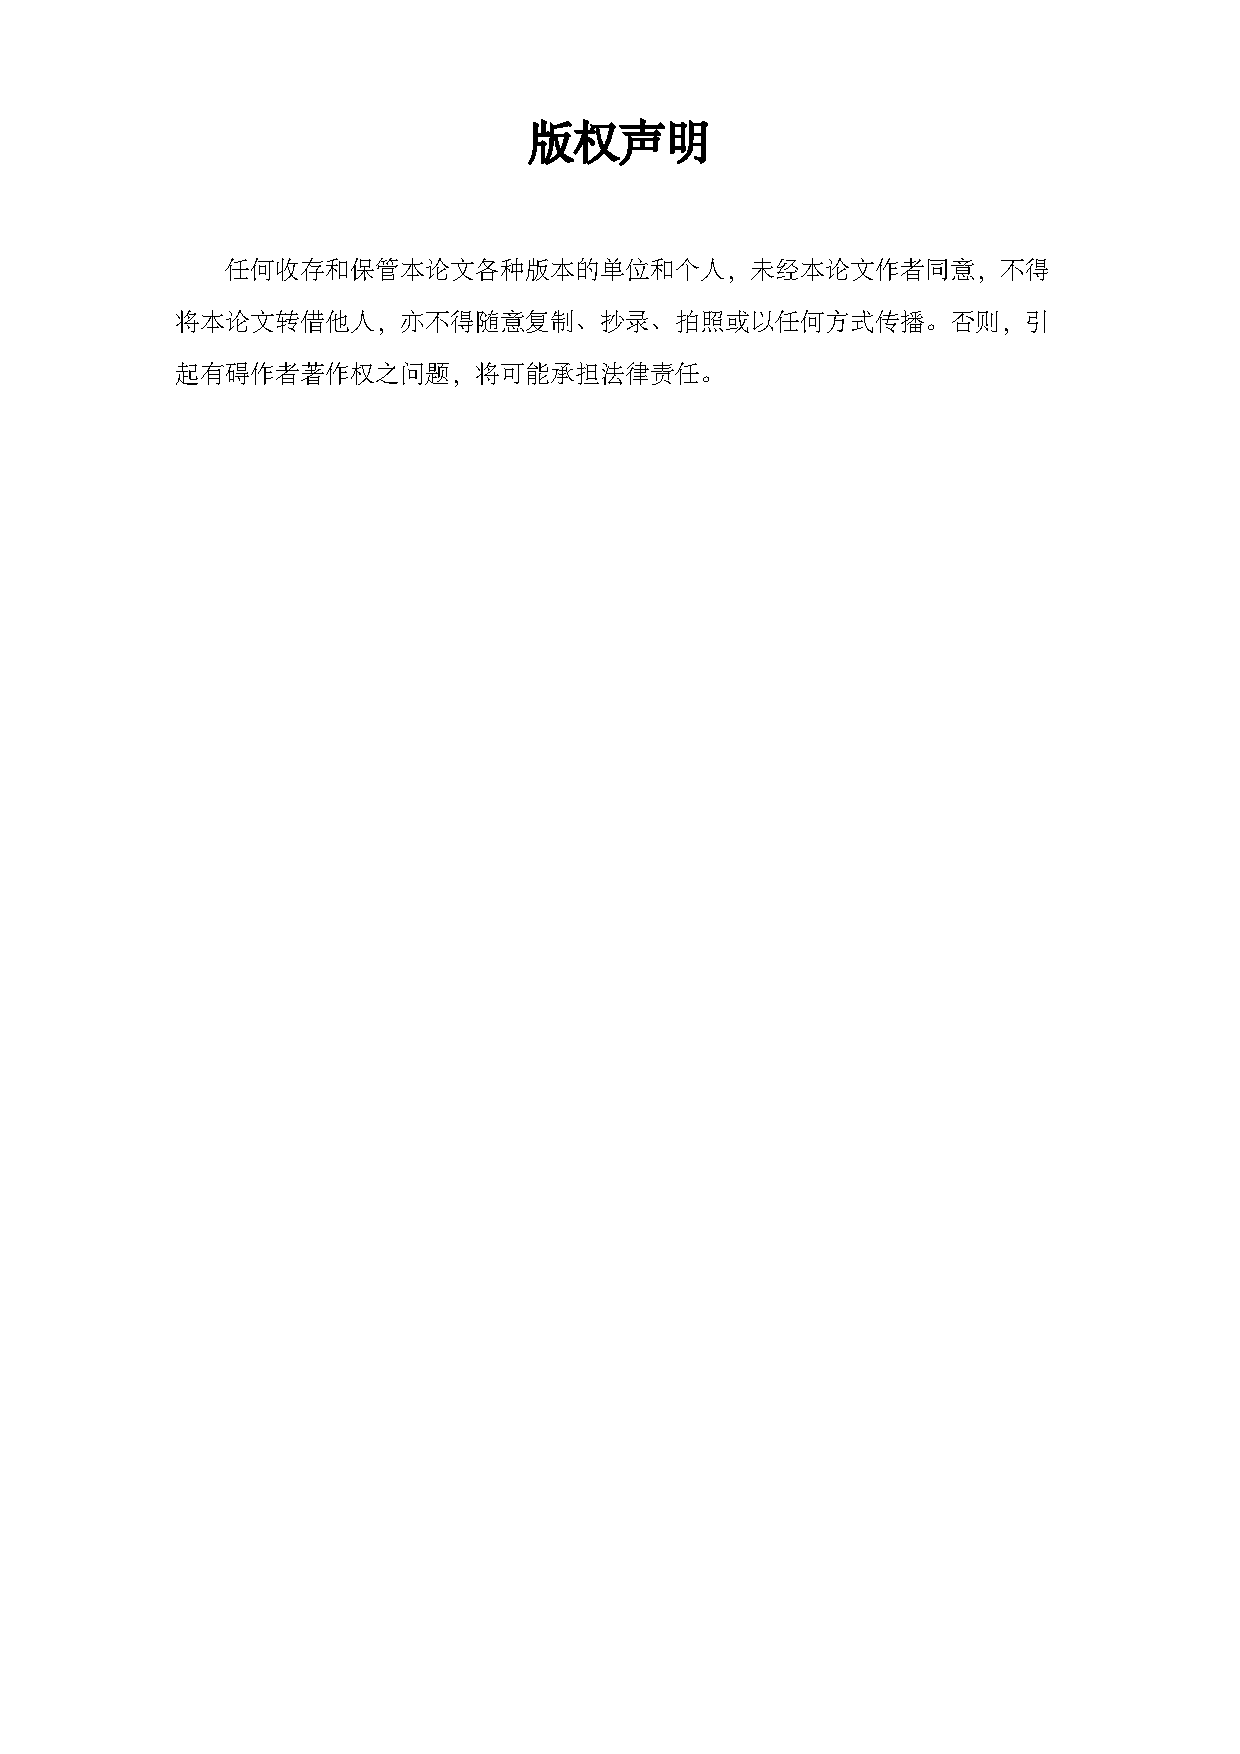
\includepdf{copyright2.pdf}
\cleardoublepage
%中文摘要
 \renewcommand{\headrulewidth}{0.75pt}
 \fancyhead[CE]{\typeyemei 北京大学硕士学位论文}
 \renewcommand{\chaptermark}[1]{\markboth{第\CJKnumber{\arabic{chapter}}章\enspace #1}{}}
 \fancyhead[CO]{\typeyemei\leftmark}
\renewcommand{\headrule}{
    {%\if@fancyplain\let\headrulewidth\plainheadrulewidth\fi
     \makeheadrule}}
% !Mode:: "TeX:UTF-8"
% 文字编码:UTF-8
%%%%%%%%%%%%%%%%%%%%%%%%%%%%%%%%%%%%%%%%%%%%%%%%%%%%%%%%%%%%%%%%%%%%%%%%%
%
%   LaTeX File for Doctor (Master) Thesis of Peking University
%   LaTeX + CJK     北京大学博士(硕士)论文模板
%   Based on Wang Lei's Template for THU
%   Version: 1.00
%   Last Update: 2005-05-25
%
%%%%%%%%%%%%%%%%%%%%%%%%%%%%%%%%%%%%%%%%%%%%%%%%%%%%%%%%%%%%%%%%%%%%%%%%%
%   Copyright 2004-2005  by  Ying Pan       (yeying_pan@yahoo.com.cn)
%%%%%%%%%%%%%%%%%%%%%%%%%%%%%%%%%%%%%%%%%%%%%%%%%%%%%%%%%%%%%%%%%%%%%%%%%
%%%%%%%%%%%%%%%%%%%%%%%%%%%%%%%%%%%%%%%%%%%%%%%%%%%%%%%%%%%%%%%%%%%%%%%%%
%
%   LaTeX File for Doctor (Master) Thesis of Tsinghua University
%   LaTeX + CJK     清华大学博士(硕士)论文模板
%   Based on Wang Tianshu's Template for XJTU
%   Version: 1.00
%   Last Update: 2003-09-12
%
%%%%%%%%%%%%%%%%%%%%%%%%%%%%%%%%%%%%%%%%%%%%%%%%%%%%%%%%%%%%%%%%%%%%%%%%%
%   Copyright 2002-2003  by  Lei Wang (BaconChina)       (bcpub@sina.com)
%%%%%%%%%%%%%%%%%%%%%%%%%%%%%%%%%%%%%%%%%%%%%%%%%%%%%%%%%%%%%%%%%%%%%%%%%

\newitemsep
\renewcommand{\labelenumi}{(\arabic{enumi})}
\cabstract{
\thispagestyle{plain}
随着移动智能设备的发展和3G、4G、WiFi等无线网络的普及,实时视频通话的使用越来越广泛,通话质量大幅度提高。另一方面,实时视频对网络质量尤其是网络延迟的高度敏感和无线网络参差不齐的网络质量之间的矛盾极大阻碍了实时视频服务质量的提升。本次课题抓住逐渐增加的高清视频通话应用的需求,研究面向无线网络的高清实时视频通话系统的实现,并解决了其中的关键算法问题。
首先,我们关注在有限并且不断波动的网络带宽下,如何及时调整视频码率从而在避免拥塞的前提下最有效地利用网络带宽。与传统拥塞控制算法(TCP、TFRC等协议)不同的是,应用于实时视频的拥塞控制算法对网络延迟有更高的要求,同时需要考虑视频数据本身的特点。为此,我们提出了一个基于排队延迟和控制论优化的拥塞控制算法,在保证网络延迟低于目标值的前提下对带宽进行更加高效稳定的利用。
其次,针对无线网络较高丢包率,而传统差错保护算法往往引入较大额外延迟的问题,我们采用了基于扩展窗口的FEC冗余保护方案,并在此基础上结合实时视频数据包重要性不同的特点,对冗余数据的分配进行了优化。利用我们的优化框架,可以在不引入额外延迟的前提下,大大提高FEC冗余保护的效果。
最后,在上述研究的基础上,我们对一个开源VOIP软件Linphone进行了系统实现。增加了新的拥塞控制算法和FEC冗余保护模块,并针对大屏电视盒子进行了界面优化。与传统实时视频应用相比,我们的软件能更好地适应无线网络特性,提供更高质量的实时视频通话。

%\quad \\ \quad \\ \quad \\ \quad \\ \quad \\ \quad \\ \quad \\ \quad \\ \quad \\ \quad \\ \quad \\ \quad
\vfill
% 当关键词与脚注(某某基金资助)在同一页时,需要人工增减“\quad \\”来保证“关键词放摘要页最下方”。另一种方法是采用\vfill,但是在package.tex中使用脚注控宏包footmisc时就不能再采用选项bottom,代价是每页的脚注底部可能不对齐。

% 当中文摘要较长,使得关键词在摘要的第二页时,采用\vfill即可使关键词位于页面底部。(与英文摘要中关键词的处理方法相同)

关键词:实时视频传输,无线网络,码率自适应,非对称差错保护
}


%英文摘要
% !Mode:: "TeX:UTF-8"
% 文字编码:UTF-8
%%%%%%%%%%%%%%%%%%%%%%%%%%%%%%%%%%%%%%%%%%%%%%%%%%%%%%%%%%%%%%%%%%%%%%%%%
%
%   LaTeX File for Doctor (Master) Thesis of Peking University
%   LaTeX + CJK     北京大学博士(硕士)论文模板
%   Based on Wang Lei's Template for THU
%   Version: 1.00
%   Last Update: 2005-05-25
%
%%%%%%%%%%%%%%%%%%%%%%%%%%%%%%%%%%%%%%%%%%%%%%%%%%%%%%%%%%%%%%%%%%%%%%%%%
%   Copyright 2004-2005  by  Ying Pan       (yeying_pan@yahoo.com.cn)
%%%%%%%%%%%%%%%%%%%%%%%%%%%%%%%%%%%%%%%%%%%%%%%%%%%%%%%%%%%%%%%%%%%%%%%%%
%%%%%%%%%%%%%%%%%%%%%%%%%%%%%%%%%%%%%%%%%%%%%%%%%%%%%%%%%%%%%%%%%%%%%%%%%
%
%   LaTeX File for Doctor (Master) Thesis of Tsinghua University
%   LaTeX + CJK     清华大学博士(硕士)论文模板
%   Based on Wang Tianshu's Template for XJTU
%   Version: 1.00
%   Last Update: 2003-09-12
%
%%%%%%%%%%%%%%%%%%%%%%%%%%%%%%%%%%%%%%%%%%%%%%%%%%%%%%%%%%%%%%%%%%%%%%%%%
%   Copyright 2002-2003  by  Lei Wang (BaconChina)       (bcpub@sina.com)
%%%%%%%%%%%%%%%%%%%%%%%%%%%%%%%%%%%%%%%%%%%%%%%%%%%%%%%%%%%%%%%%%%%%%%%%%

%%%%%%%%%%%%%%%%%%%%%%%%%%%%%%%%%%%%%%%%%%%%%%%%%%%%%%%%%%%%%%%%%%%%%%%%%
%
%   LaTeX File for xi'an Jiao Tong University
%
%%%%%%%%%%%%%%%%%%%%%%%%%%%%%%%%%%%%%%%%%%%%%%%%%%%%%%%%%%%%%%%%%%%%%%%%%
%   Copyright 2001  by  Wang Tianshu    (tswang@asia.com)
%%%%%%%%%%%%%%%%%%%%%%%%%%%%%%%%%%%%%%%%%%%%%%%%%%%%%%%%%%%%%%%%%%%%%%%%%
\newitemsep
\renewcommand{\labelenumi}{(\arabic{enumi})}
\eabstract{
\thispagestyle{plain}

With the popularity of camera-ready mobile devices and 3G/4G/WiFi wireless infrastructure, interactive video applications with wireless Internet access links are growing exponentially. However, real-time video streaming over wireless networks still faces many challenges such as varying latency, bandwidth fluctuation, and wireless physical packet losses. In this research, we focus on the quality of service (QoS) improvement of real-time video streaming over wireless networks.
Firstly, we propose a delay-constraint rate control algorithm for real-time video streaming over wireless networks.We first introduce a fluid-queueing model to explore the insight of network congestion. By maintaining a desired number of packets in network queue, we can achieve high bandwidth utilization and low transmission delay. To make rate control more stable and agile, a closed-loop rate control system is designed employing a Proportional-Integral (PI) controller and the control parameters are analyzed using a control-theoretic approach.
Then, we adopted an expanding window reed-solomon code, and introduce an equivalent error probability to simplify them. Then we are able to formulate the optimal redundancy allocation into a constrained nonlinear optimization problem, where by allocating the redundancy unequally considering the unequal importance of different frames and their dependency based on the expanding window, unequal error protection (UEP) is achieved and the overall distortion is minimized.
Based on the research above, we made refactoring of an open source VOIP software named Linphone, implemented new modules for rate control and error control, and optimized the UI to fit for TV screen. Compared to traditional real-time video streaming applications, our implementation adapts better with wireless networks and provides higher quality of video streaming.

\vfill
KEYWORDS: Real-Time Video Streaming, Wireless Networks, Rate Control, Error Control, Real-Time Video System
}

\makeabstract

% 对应于小四的标准字号是 12pt
% 可以在正文中用此命令修改所需要字体的的大小
% 下面这个设置是正文各章使用的标准字体与行距
\renewcommand{\baselinestretch}{1.2}
\fontsize{12pt}{20pt}\selectfont

%目录
\tableofcontents
%\thispagestyle{empty}

\cleardoublepage
%表格目录
%\listoftables
%\thispagestyle{empty}

%插图目录
\listoffigures
%\thispagestyle{empty}

%符号对照表
%\include{preface/denotation}

\cleardoublepage

%设置列表的行距

\renewcommand{\labelenumi}{(\arabic{enumi})}
\newitemsep

%--- body --------------------------
\mainmatter


%正文章节

%\pagenumbering{arabic}
%\renewcommand{\thefootnote}{\arabic{footnote}}

%绪论
% !Mode:: "TeX:UTF-8"
% 文字编码:UTF-8
\chapter{引言}
\label{chap:intro}
随着带有摄像功能的便携智能设备的发展,以及各种无线网络覆盖率的提升,视频通话越来越多地应用在人们的日常生活中,如可视电话、视频会议、远程医疗、在线直播等。实时视频传输对网络质量要求较高,而目前无线信道存在的带宽波动、延迟、丢包等问题,使其面临很多困难和挑战。如何在多样化的网络环境下提供稳定和高质量的视频服务越来越成为工业界和学术界关注的热点。为此,本课题针对在无线网络上保障实时视频传输的质量,以及实现高可用性的视频通话系统进行研究。

\section{研究背景及意义}
人类通信的发展经历了飞鸽传书,邮寄信件,电报,固定电话,移动电话等阶段。在互联网出现后,又涌现出Email,网络语音,网络视频等更加方便快捷的通信形式,而移动互联网的发展更使人们随时随地都可以实现语音、视频通信。根据Cisco发布的全球移动数据预测报告\cite{index2016global},过去的2015年中全球移动网络数据流量增长了74\%,达到每个月3.7 艾字节,而到2020年这一数字预计将达到每个月30.6艾字节,人们对于移动互联网的依赖可见一斑。另一方面,如图\ref{fig:cisco_mobile}所示,2015年移动网络数据流量中,视频数据占比重为55\%,到2020年预计为75\%,以62\%的年均增长率成为移动网络中的绝对主流。可以想见,视频通话由于其实效性和丰富的信息量,必将成为人们日常通信的最主要方式。而无线网络作为便捷的网络接入方式,也将成为视频传输的最重要媒介。

与此相应的是,实时视频服务相关的产品和市场也蓬勃发展起来。日常通信方面,FaceTime、Skype、米聊等内置软件提供的视频聊天功能几乎成了智能手机系统的标配,而QQ、微信、环聊等社交软件也纷纷加入视频聊天功能,以此为基础的小游戏、互动软件也不断被开发出来。在企业全球化的今天,视频电话会议、远程医疗等也成为各大公司必备的生产力工具,具有极大的市场潜力。

近年来,电视盒子作为一种全新的互联网接入设备逐渐普及,使得电视机从单纯的电视节目播放转变成为家庭多媒体终端。除了观看网络视频以外,一些电视盒子还提供了视频通话功能,利用电视机高清大屏进行高质量的视频聊天。这一基于电视盒子的大屏视频通话,可以应用在日常通信、娱乐,视频会议,家庭监控等不同场景,具有较高的研究价值。当然电视盒子一般通过家庭Wi-Fi接入互联网,视频聊天的效果也会受到无线网络一些不利因素的限制。
总之,越来越高清的视频质量和多样化的服务需求,给无线网络下的实时视频数据的高效传输提出了巨大挑战。

\begin{figure}[htbp]
  \centering
  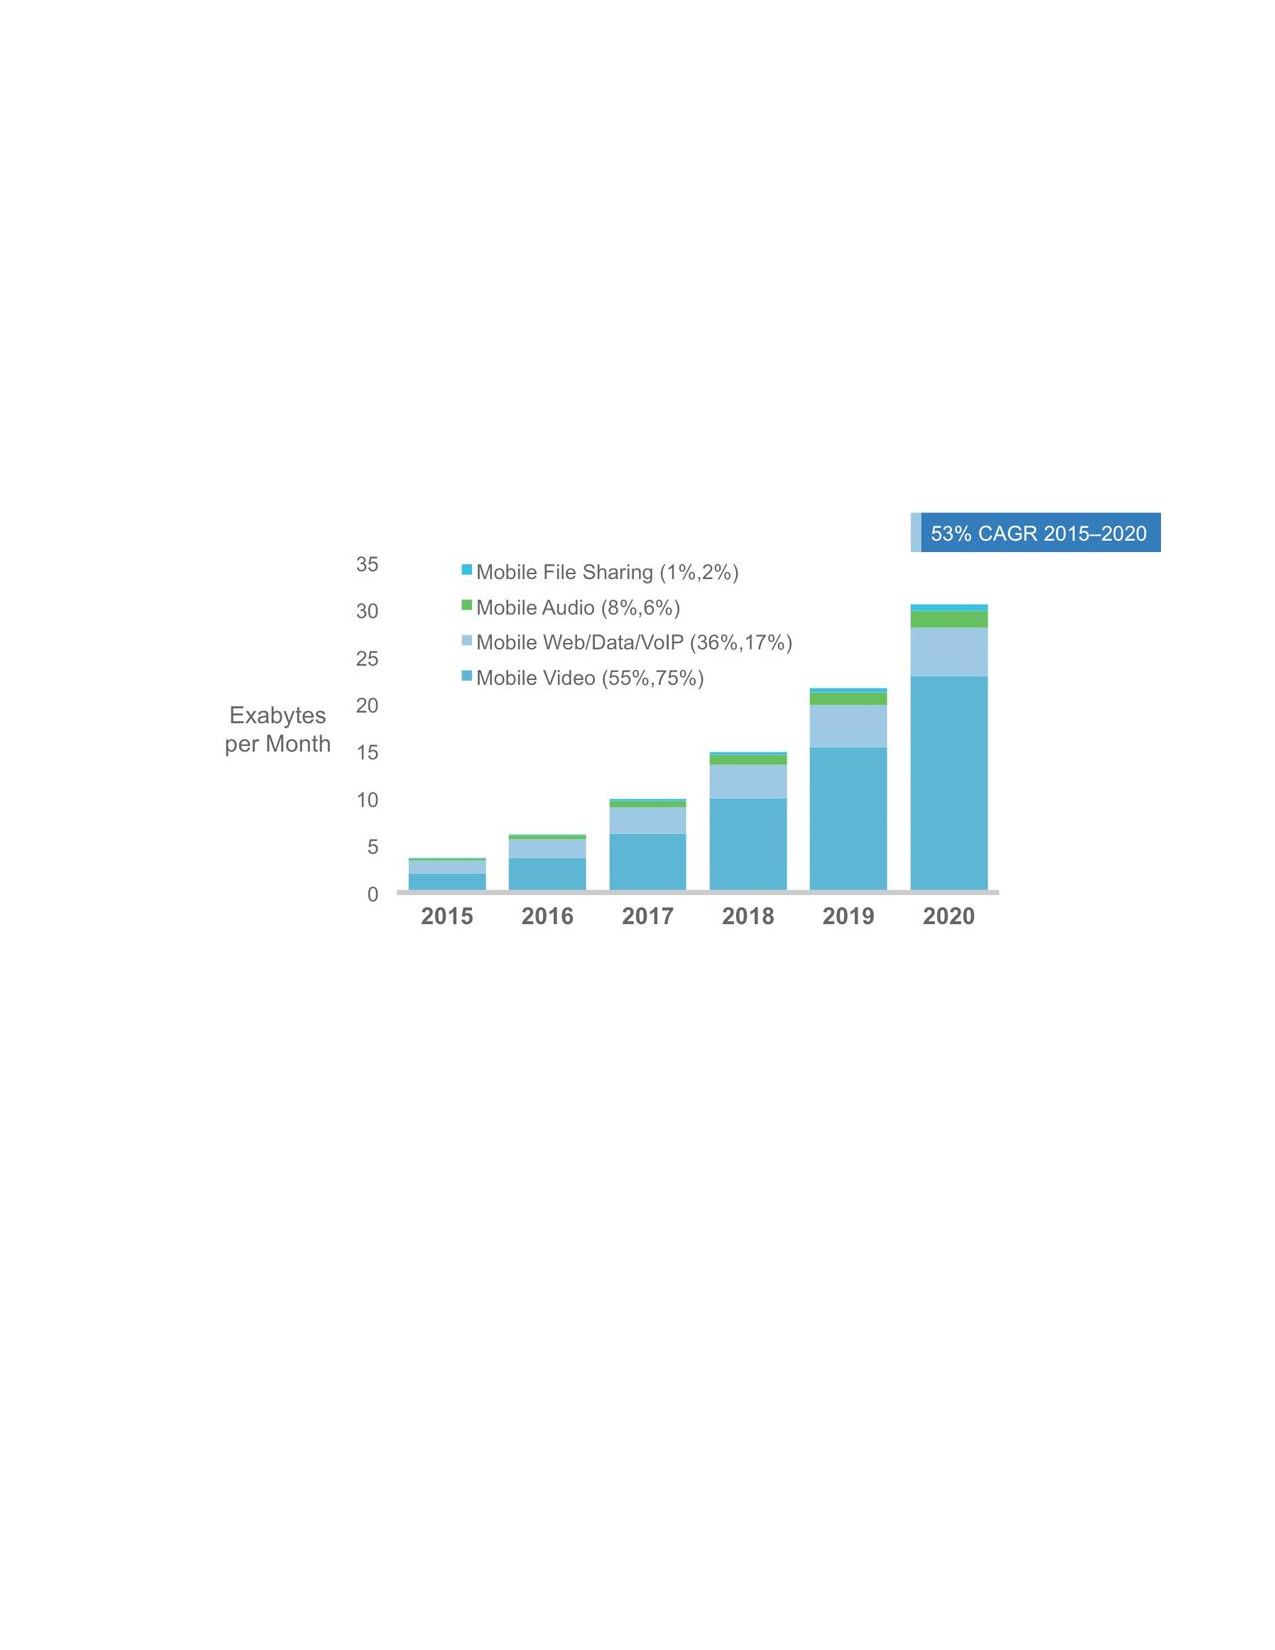
\includegraphics[width=0.83\textwidth]{cisco_mobile_traffic.pdf}
  \caption{2020年移动视频流量预测}
  \label{fig:cisco_mobile}
\end{figure}

高质量的视频通话体验依赖于较高的视频编码码率,较低的传输延迟,以及稳定可靠的传输信道。其中任何一项不满足,都会对用户体验造成很大的影响。而在网络传输方面,由于实时性的限制,基于重传的传统TCP协议并不适用于实时视频的传输,大部分实时视频传输都使用了面向数据包的UDP传输协议,在UDP协议层并没有对数据传输进行任何质量保障。无线网络信道的不稳定性,以及终端设备的多样化,也增加了实时视频的传输优化和质量保证的难度。具体来说,在无线网络中进行实时视频传输面临的主要问题包括:

\begin{itemize}
    \item 有限的网络带宽与越来越高的带宽需求之间的矛盾。视频数据信息量丰富,对网络带宽的需求也很大,过低的带宽会引起视频画面模糊、延迟增加,如果带宽低于视频最低压缩码率,则完全无法进行视频通话。同时为了保证通话过程中画面稳定,对带宽的波动也有一定限制。而无线网络由于终端位置移动、信号衰减等因素,带宽波动很大。
    \item 视频通话对延迟的高度敏感。由于视频通话涉及双方交互,轻微的延迟就会造成明显的通话不连贯。另一方面,为了保证视频播放连续性,每个视频包都需要在相应视频帧播放之前到达,否则就与丢包无异。而无线网络由于信道不稳定,本身存在一定的延迟。并且如果由于带宽波动引发网络拥塞,将产生更大的延迟。
    \item 网络丢包影响视频质量。由于视频文件编码特性,轻微的数据错误都可能造成连续画面的明显失真甚至无法解码。而无线网络下由于信号强度变化、终端移动等,发生数据错误和丢包概率大大增加。
\end{itemize}

针对以上实时视频传输和无线网络质量之间的一系列矛盾,视频码率自适应和非对称差错保护这两种技术可以在很大程度上对其进行改善,具体体现在:

\begin{itemize}
    \item 通过码率自适应算法及时合理地调整视频码率,可以保证网络负载始终稳定在网络承载能力以下,在实现较高带宽利用率的同时避免网络拥塞。既避免了网络拥塞引起延迟增大、丢包等影响视频传输质量的问题,又提高了视频平均码率。
    \item 对于信道不稳定造成的丢包,通过非对称差错保护添加冗余信息,可以为数据传输提供一定容错能力。使视频传输在高丢包环境下也能获得稳定的观看效果。
\end{itemize}

下面我们将介绍本文算法和系统中涉及到的一些基本概念。

\subsection{无线网络简介}
无线网络是指通过无线电波作为媒介进行传播的信息网络,一般我们提到的无线网络都与互联网相连,为用户提供移动互联网访问的能力。随着手机、笔记本电脑等移动智能设备数量激增,当今无线网络在技术、覆盖率等方面都有了极大的发展,其中蜂窝网络(如3G、4G)和无线局域网(Wi-Fi)是目前应用最广泛的无线网络。无线网络具有架设快速、接入灵活、使用方便等优点,已经深入到人们生活的方方面面。本文关注的实时视频通信,其大部分应用场景都发生在手机蜂窝网络和家庭Wi-Fi环境下。尽管如此,在无线网络的使用中仍然存在很多问题 \cite{heusse2003performance},包括:
\begin{itemize}
    \item 信号干扰:相比有线系统,无线网络经常受到电磁干扰,如其他无线网络或电磁设备等。这些干扰可能导致无线网络信号衰减、数据丢失等问题。
    \item 信号吸收和反射:无线信号在传播过程中会被某些材料吸收或反射,在覆盖范围内造成信号死角。
    \item 资源竞争:无线频谱是有限的资源,并由发射范围内的所有节点共享。如果多个无线网络出现频谱冲突,会造成网络带宽下降、延迟增加等问题。而随着无线网络需求增加,这一冲突的发生概率也越来越大。
\end{itemize}

在以上问题的背景下,无线网络下的视频传输需要解决带宽波动大、高丢包率、高延迟等问题,这对于视频通话系统的设计、算法优化都提出了特殊的要求。


\subsection{实时视频传输基本框架}

\begin{figure}[htbp]
  \centering
  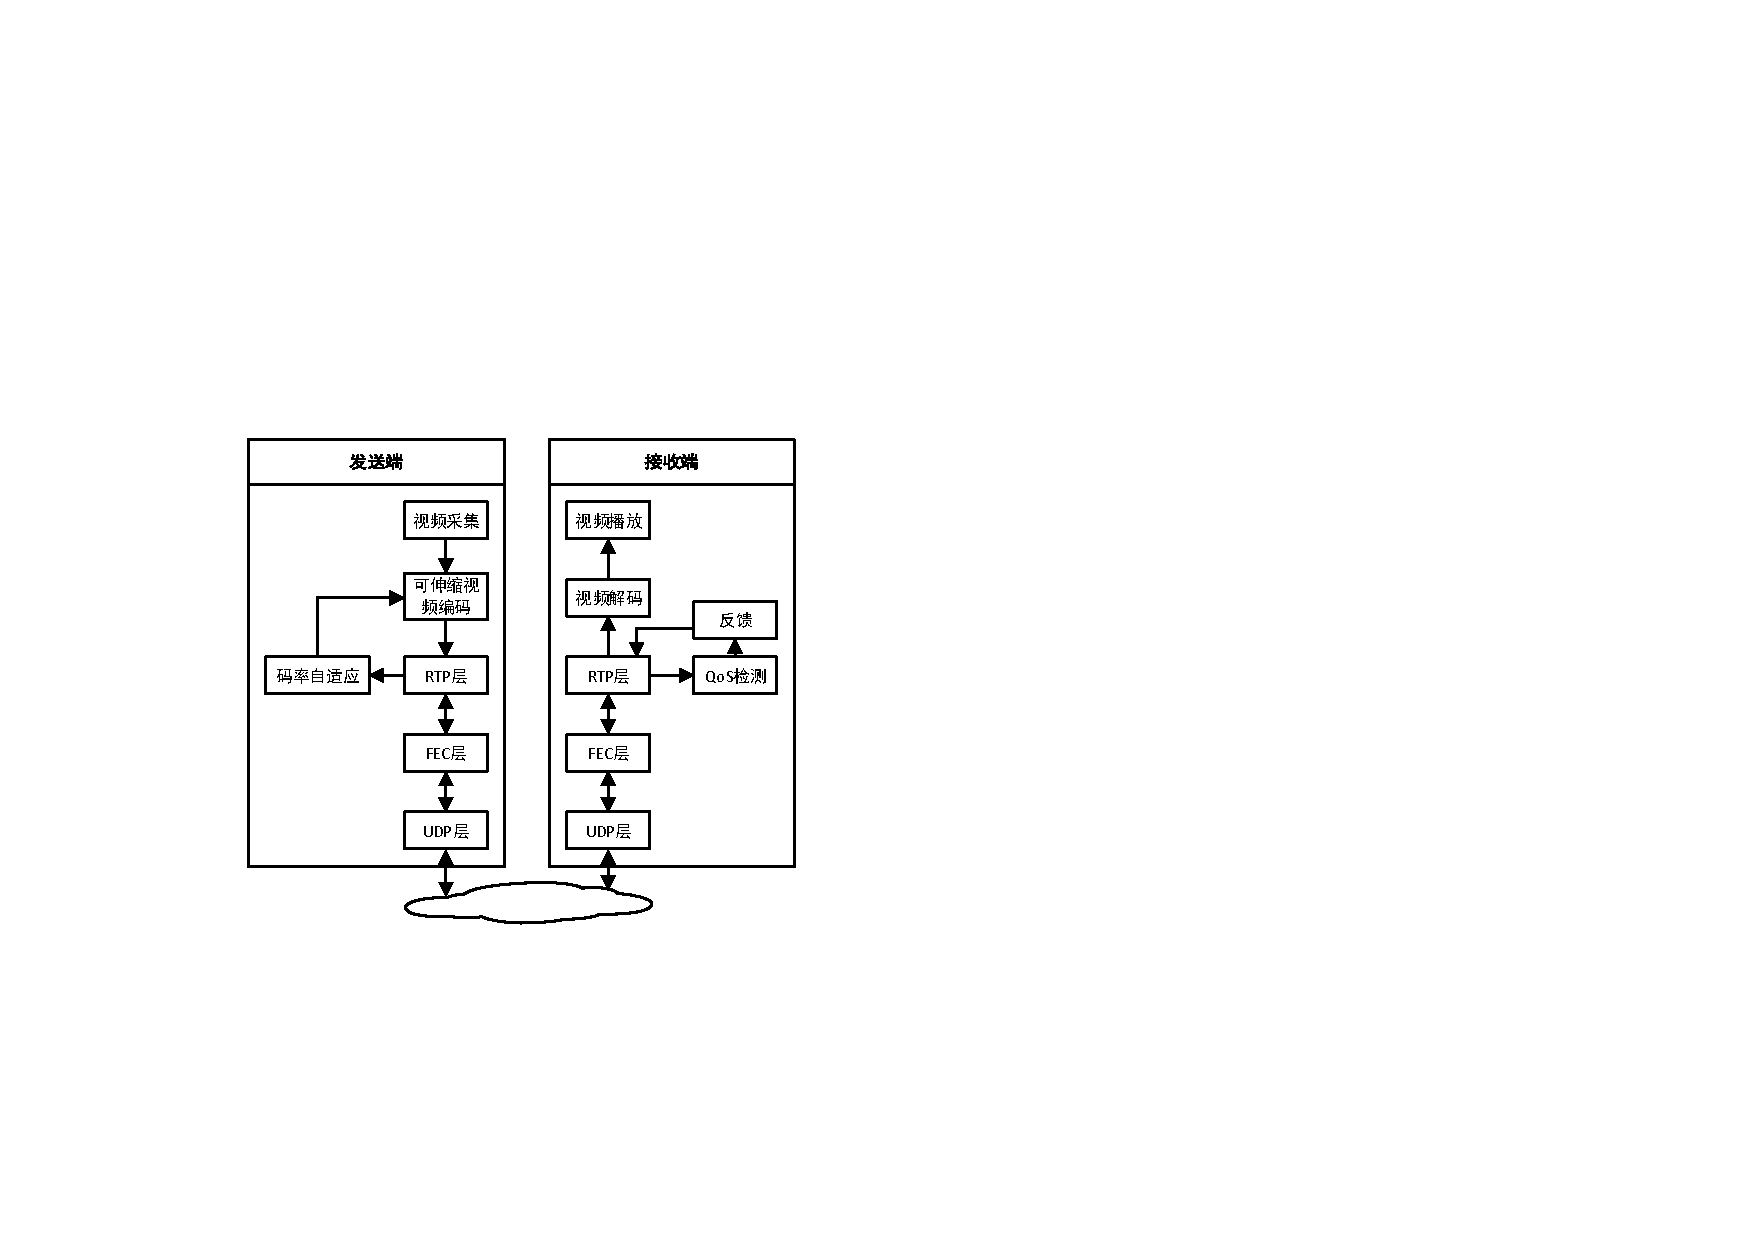
\includegraphics[width=0.75\textwidth]{steaming_architecture.pdf}
  \caption{实时视频传输基本框架图}
  \label{fig:steaming_architecture}
\end{figure}

尽管不同的实时视频通话应用实现方式千差万别,他们却有着基本相同的功能单元和整体架构,一个基本的实时视频传输系统框架如图 \ref{fig:steaming_architecture} \cite{wu2000transporting}所示。在发送端,视频采集模块通过摄像头等设备将自然场景转换为数字信号;可伸缩视频编码模块采用VP8、H.264等协议对原始视频信号进行压缩编码处理,生成码率可变的视频数据流;为了完成流式传输和观看,视频数据还需要在RTP层经过Real-time Transport Protocol(RTP)协议 \cite{jacobson2003rtp} 封装,添加序列号、时间戳等信息才能正确地在接收端实时解码和播放;为了应对丢包造成的失真,还可以在发送前对数据包进行FEC编码以添加冗余保护信息(可选);最后,数据由UDP层封装,通过更底层网络接口发送到接收端。这些数据包可能由于发生拥塞在网络链路上被丢弃,或由于超时而被接收端丢弃。接收端成功接收的数据包,经过一系列拆包、解码,还原为视频图像信息,并按照预定时间戳播放。

无线网络信号质量千差万别,其提供数据传输的能力也各不相同,这就要求通话双方根据网络状况合理选择发送视频的码率。为此,在实时视频传输系统框架中一般还加入了位于接收端的Quality of Service(QoS) 检测和反馈模块,用于检测当前通信信道的可用带宽、网络延迟、丢包率等信息;反馈模块将这些信息通过RTP协议附带的控制协议发送给接收端的码率自适应模块,在发送端根据不同的码率调整策略改变输出视频的码率,从而实现网络拥塞避免和网络带宽的有效利用。


\subsection{视频码率自适应}
在视频编码过程中,通过设定不同的分辨率、帧率、压缩倍数等,可以动态改变输出视频数据流的码率。例如在较差的网络条件下使用较低的视频码率,虽然损失了一定的画面清晰度,但是由于带宽需求更低,至少能够保证通话过程的平滑流畅。而在带宽充足的情况下,使用较高的视频码率可以充分利用带宽,提供更清晰的视频画面。利用这一思路,通过在通话过程中不断调整视频码率,可以在保证通话顺利进行的前提下,尽可能提高网络带宽利用率,从而获得更好的视频体验。然而这一调节过程本身存在矛盾:如果过分强调带宽利用率,采取激进的码率策略,一旦网络出现波动很容易造成拥塞;而过于保守的码率策略则会造成带宽浪费。因此如何根据网络状况准确调节视频码率,是进行视频传输需要重点解决的问题。

另一方面,实时视频作为一种实时流媒体,与一般网络数据传输最大的不同就是它对数据实时性的要求,一旦数据到达时间超过了有效播放时间,则与丢包无异。而网络上应用最广泛的 TCP 传输协议通过维护拥塞窗口以及丢包重传机制保障数据传输的可靠性,却也因此引入了较大的传输延迟,并不适用于网络上比重越来越大的实时流媒体传输。这就要求我们为实时视频传输设计专门的码率自适应算法。

\subsection{视频传输的非对称差错保护}
实时视频传输和普通文件传输的一个重要区别就是,视频数据即使发生了部分错误,仍然可以继续播放,只是部分画面会出现马赛克或丢帧,降低一定的用户体验。因此在很多视频通话应用中,差错控制模块都属于可选模块。但如果视频传输在高丢包率的无线网络条件下进行,过多的丢包就会对视频质量造成严重影响,需要通过一定的差错控制措施来减少丢包造成的质量损失。最常用的实时视频传输差错保护方法就是FEC冗余编码,通过向发送数据流中加入冗余信息提供一定纠错能力,在接收端即使只收到部分数据,仍然有可能解码出原始信息。

由于视频编码过程中进行了数据压缩,一个视频流中不同的数据重要性一般是各不相同的。有些数据一旦丢失会造成多个视频帧无法解码,而有些数据只会造成某一帧画面上的少量失真。一种直观的想法是在FEC冗余编码过程中重点保护那些更重要的数据,为它们分配更多的冗余信息。这种根据数据重要程度不同进行不同程度保护的策略成为非对称差错保护。而冗余信息分配是否合理,也在很大程度上影响了冗余保护的效果。因此研究视频传输的非对称差错保护,是提升视频通话质量的一种有效途径。

另外,在FEC编解码过程中,单个编码块的大小(即一次编码所包含的数据包数量)对于编解码效果有很大影响。编解码单元越大,FEC编解码效率越高,灵活性也越好。然而如果采用较大的编解码单元,在发送端需要等待编码块中数据包涉及到的视频帧全部编码完毕才能进行FEC 编码,接收端则需要等待编码块中所有数据包接收完毕才能实现FEC解码,这都会引入额外的编解码延迟,从而对延迟敏感的实时视频传输产生较大影响。因此如何在不引入额外延迟的前提下提升FEC编解码效率也是实现差错保护过程中需要关注的问题。

\section{研究内容}
\begin{figure}[htbp]
  \centering
  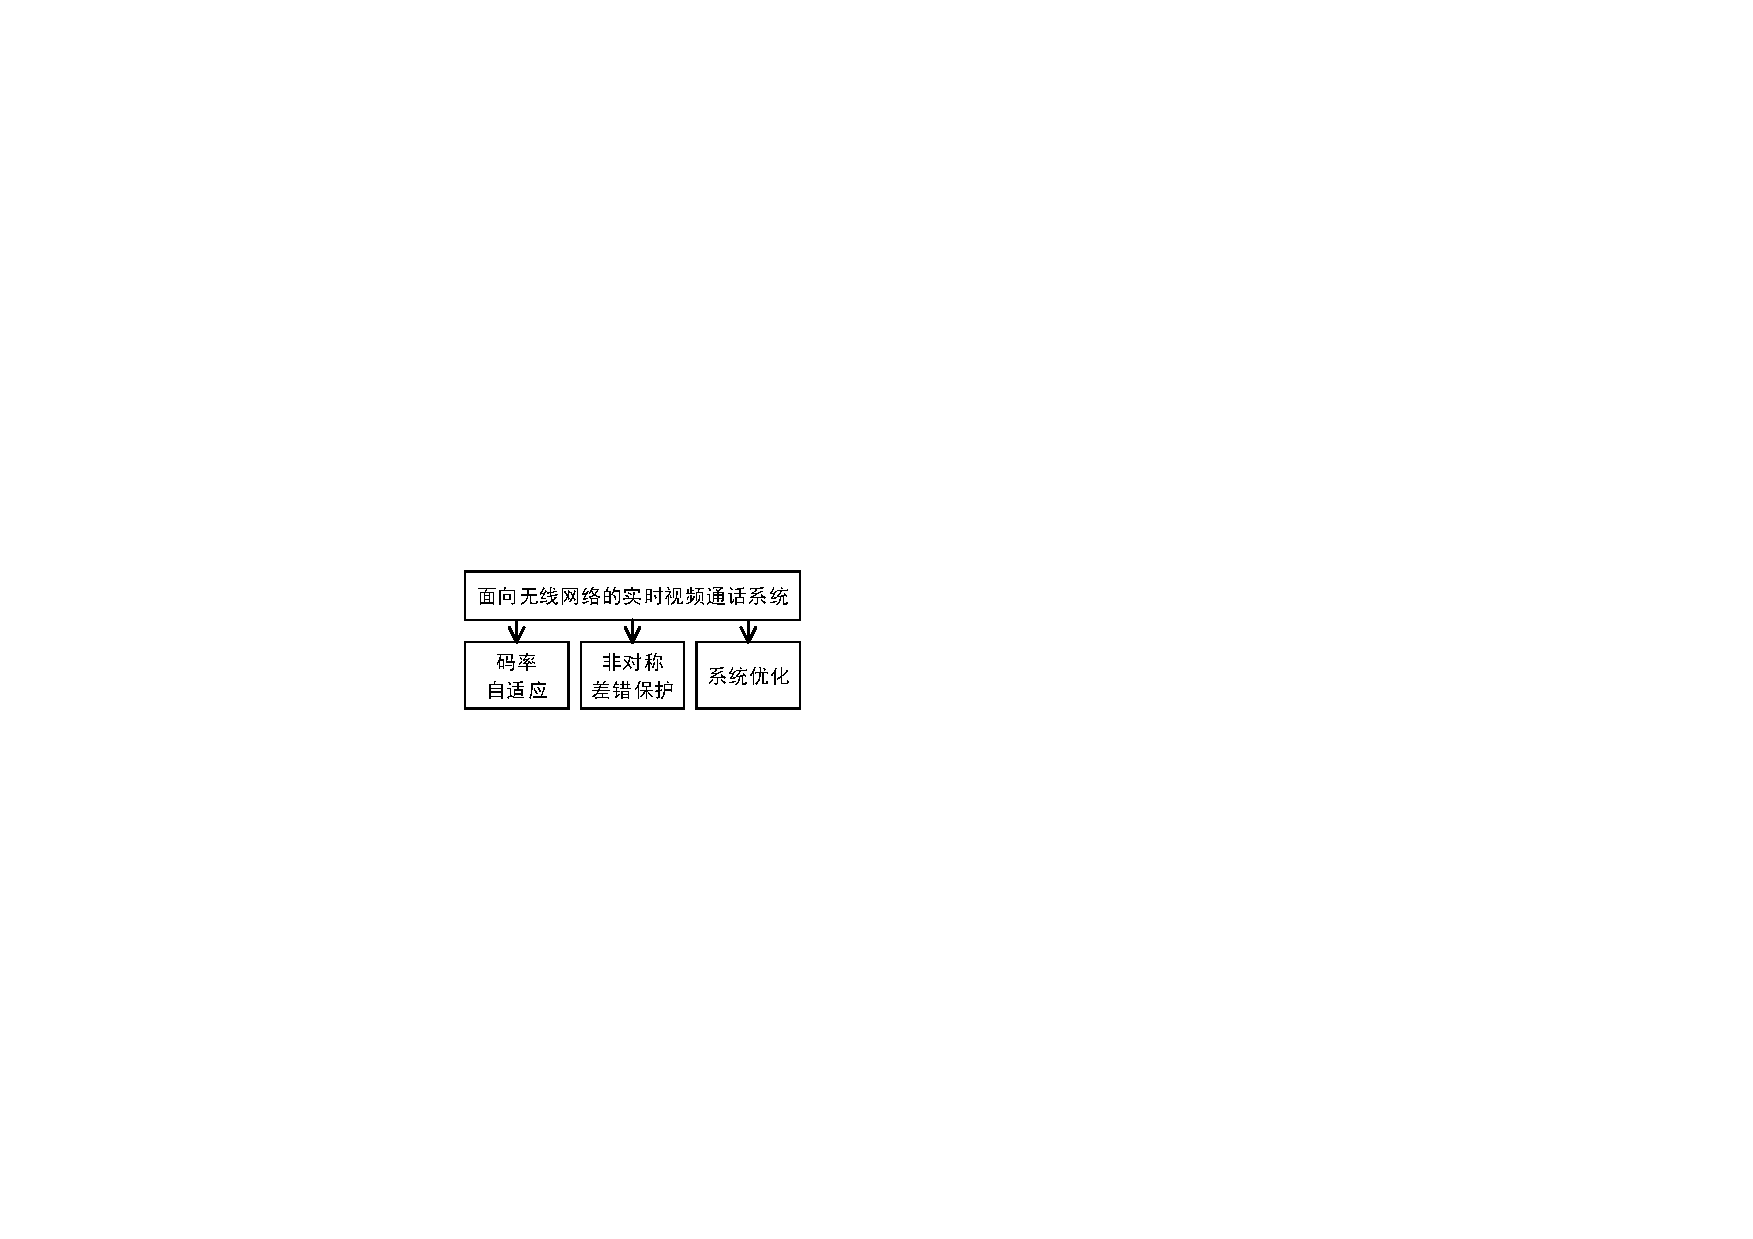
\includegraphics[width=0.46\textwidth]{research_architecture2.pdf}
  \caption{研究框架}
  \label{fig:research_architecture}
\end{figure}

基于上述背景,我们希望实现一个能够在无线网络中提供高质量服务的实时视频通话应用,同时结合电视盒子大屏幕的特性提供高清视频通话服务。我们以图 \ref{fig:steaming_architecture}中的实时视频传输基本框架为原型,基于开源VoIP软件Linphone搭建了面向电视盒子的实时视频传输原型系统。
该系统中对通话质量影响最大的就是复杂网络状况下视频码率的确定,以及高丢包环境下如何保证视频解码成功率。

针对上述问题,我们以图 \ref{fig:research_architecture}为研究框架,在以下几个方面展开研究:
首先,为了在网络带宽不稳定、丢包和延迟都更加严重的无线网络下实现稳定的视频传输,我们提出一种基于排队延迟的码率自适应框架,实现延迟可控的视频传输,并用控制论模型对调整过程进行优化;
然后,为了减小无线网络高丢包率对视频质量的影响,我们引入了非对称差错保护模块,并对非对称差错保护算法中的冗余分配这一关键环节进行了优化;
最后,综合上述算法,我们对视频通话系统的实现细节进行了优化,对界面进行改进,以提高大屏幕电视界面下的视频通话质量和用户交互体验。

\subsection{延迟优化的实时视频码率自适应算法}
高质量的实时视频传输服务要求较大且稳定的带宽、低延迟和低丢包率等,这对于网络拥塞控制也就是视频的码率自适应算法提出了很高的要求。而大部分现有拥塞控制算法主要着眼于避免网络拥塞和整体流量的公平,单个数据流获取到的带宽和网络延迟往往存在很大的波动,这极大降低了实时视频的用户体验。
尤其是在无线网络的背景下,没有进行过专门优化的码率自适应算法往往无法适应高丢包率的环境,存在带宽低估、延迟过大等问题。

本研究通过排队延迟模型对网络进行建模,分析排队延迟变化与视频码率之间的关系,进而以网络延迟为反馈信号动态调整视频码率。
另外通过引入控制论模型和PID控制器对码率调整过程进行优化,合理权衡系统稳定性和响应速度,进一步提高了码率自适应的效果。
大量实验结果表明,该码率自适应算法在带宽利用率和码率稳定性方面的表现均超过了已有主流方法,同时在传输过程中保持了较低的网络延迟,特别适用于实时流媒体的传输。
相关研究成果已发表于IEEE VCIP-2015。

\subsection{基于非对称差错保护的冗余分配优化算法}
基于扩展窗口的FEC技术具有不引入额外延迟,控制失真扩散等特点,特别适合无线网络上的实时视频传输。具体来说,考虑到视频数据的非对称特性,我们可以对差错保护效果与冗余分布的关系进行数学建模,求解最优的冗余信息分配策略,来优化差错保护的效果。而由于扩展窗口的引入,这一优化问题变得层层嵌套,十分复杂,直接求解的难度很大。

本文针对扩展窗口FEC框架中冗余数据的分配问题进行研究,提出一种基于此框架的冗余分配方案。我们首先针对扩展窗口编解码的数据包进行等效丢包率分析,并针对其编解码特征提出了关于数据包解码条件的两条推论。然后我们推导出了GOP整体语预期失真公式,作为冗余最优化分配的理论基础。在此基础上,冗余分配问题被归纳为带约束的非线性优化问题,并用简化了复杂度的贪心算法进行求解。大量实验结果表明,应用本算法得到的冗余分配策略进行扩展窗口FEC冗余保护,在各种网络场景下都能明显提高视频传输的FEC 保护效果。相关研究成果已经发表于IEEE ICIP-2015。

\subsection{面向电视盒子的实时视频通话系统}
在上述算法研究的基础上,我们以一个开源VOIP软件为基础,对其底层码率自适应模块进行重写并添加FEC差错保护模块,同时重写用户交互界面,实现了一个面向电视盒子的视频通话软件。首先在底层RTP 和RTCP 协议的基础上实现了一个码率自适应模块,以当前网络的延迟和丢包信息为输入,根据本文提出的码率自适应算法实时调整视频码率。另外,我们还实现了一个独立的差错保护模块,对底层RTP 包进行基于扩展窗口框架的FEC冗余编码和解码,在网络丢包时对视频数据进行恢复,从而更好地适应高丢包率的无线网络环境。最后,考虑到电视盒子的普及和未来视频通话的发展趋势,我们还将这一系统移植到电视盒子上,为家庭用户提供更加高质量的大屏视频通话体验。

\section{论文结构}
本论文的结构安排如下。
第 \ref{chap:intro}章首先介绍了论文的研究背景和意义,以及相关领域面对的挑战。
第 \ref{chap:related}章介绍了实时视频码率自适应和视频流差错保护方面的国内外研究现状。
第 \ref{chap:rate}章以现有拥塞控制算法为基础,考虑实时视频服务对延迟的需求,提出了一种延迟优化的码率自适应算法。
第 \ref{chap:fec}章考虑在易丢包的无线网络下进行视频传输的需求,提出一种视频流非对称差错保护中的冗余分配算法。
综合以上两种算法,我们在第 \ref{chap:system}章设计了一个面向电视盒子的高清视频通话系统。
最后在第 \ref{chap:conclusion}章对本文进行总结和未来工作的展望。

% !Mode:: "TeX:UTF-8"
% 文字编码:UTF-8
\chapter{相关研究工作}
\label{chap:related}

\section{实时视频传输码率自适应算法}
自互联网诞生以来,数据传输过程中的拥塞控制就一直是研究的重点。传统拥塞控制方法,如TCP,通过拥塞窗口 \cite{jacobson1988congestion} 控制数据传输过程,拥塞窗口的大小决定了当前能发送的数据数量。为了探测网络带宽,拥塞窗口缓慢增加,一旦检测到网络拥塞,则大幅度降低窗口大小,以求迅速恢复。Wu \cite{wu2000end}等人指出,大部分基于拥塞窗口的控制算法都包含了数据包的重传,因此不适用于对延迟敏感的实时数据传输。为了适应实时数据传输的需要,Turletti \cite{turletti1996videoconferencing} 等人提出了一种基于码率调整的拥塞控制方法,这一方法直接估计当前网络带宽并以此设置数据发送速率。结合视频编码码率可变的特性,这一基于码率的拥塞控制方法也成为实时视频码率自适应算法的基础。

\begin{algorithm}[htbp]
\caption{基于丢包率的AIMD算法}
\label{al:aimd}
    \begin{algorithmic}
    \If {$(P_{loss} \le P_{threshold})$}
        \State $r := min\{(r+AIR), MaxRate \} $
    \Else
        \State $r := max\{(\alpha * r), MinRate \} $
    \EndIf
    \end{algorithmic}
\end{algorithm}

尽管TCP由于重传机制无法被实时视频传输采用,但其对网络带宽上限进行探测的思路却在视频码率自适应算法中得到了继承。一种经典思路就是以网络丢包率作为拥塞信号对码率进行调整,如 \cite{wu2000end} 中采用的算法 \ref{al:aimd}。
其中$P_{loss}$为当前丢包率,$P_{threshold}$为判断网络拥塞的丢包率阈值,$r$是发送数据的码率,$AIR$为每次码率增加的数值。容易看出这是一种``加性增,乘性''(Additive Increase Multiplicative Decrease, AIMD)的策略,与之相应的还有研究 \cite{turletti1996videoconferencing} 中提出的``乘性增,乘性''(Multiplicative Increase Multiplicative Decrease, MIMD)策略。由于检测到丢包率明显上升时,说明网络拥塞已经发生,因此上述方法都需要通过``乘性减''策略保证码率下降速度足够快,以使网络尽快从拥塞中恢复。

\begin{figure}[htbp]
  \centering
  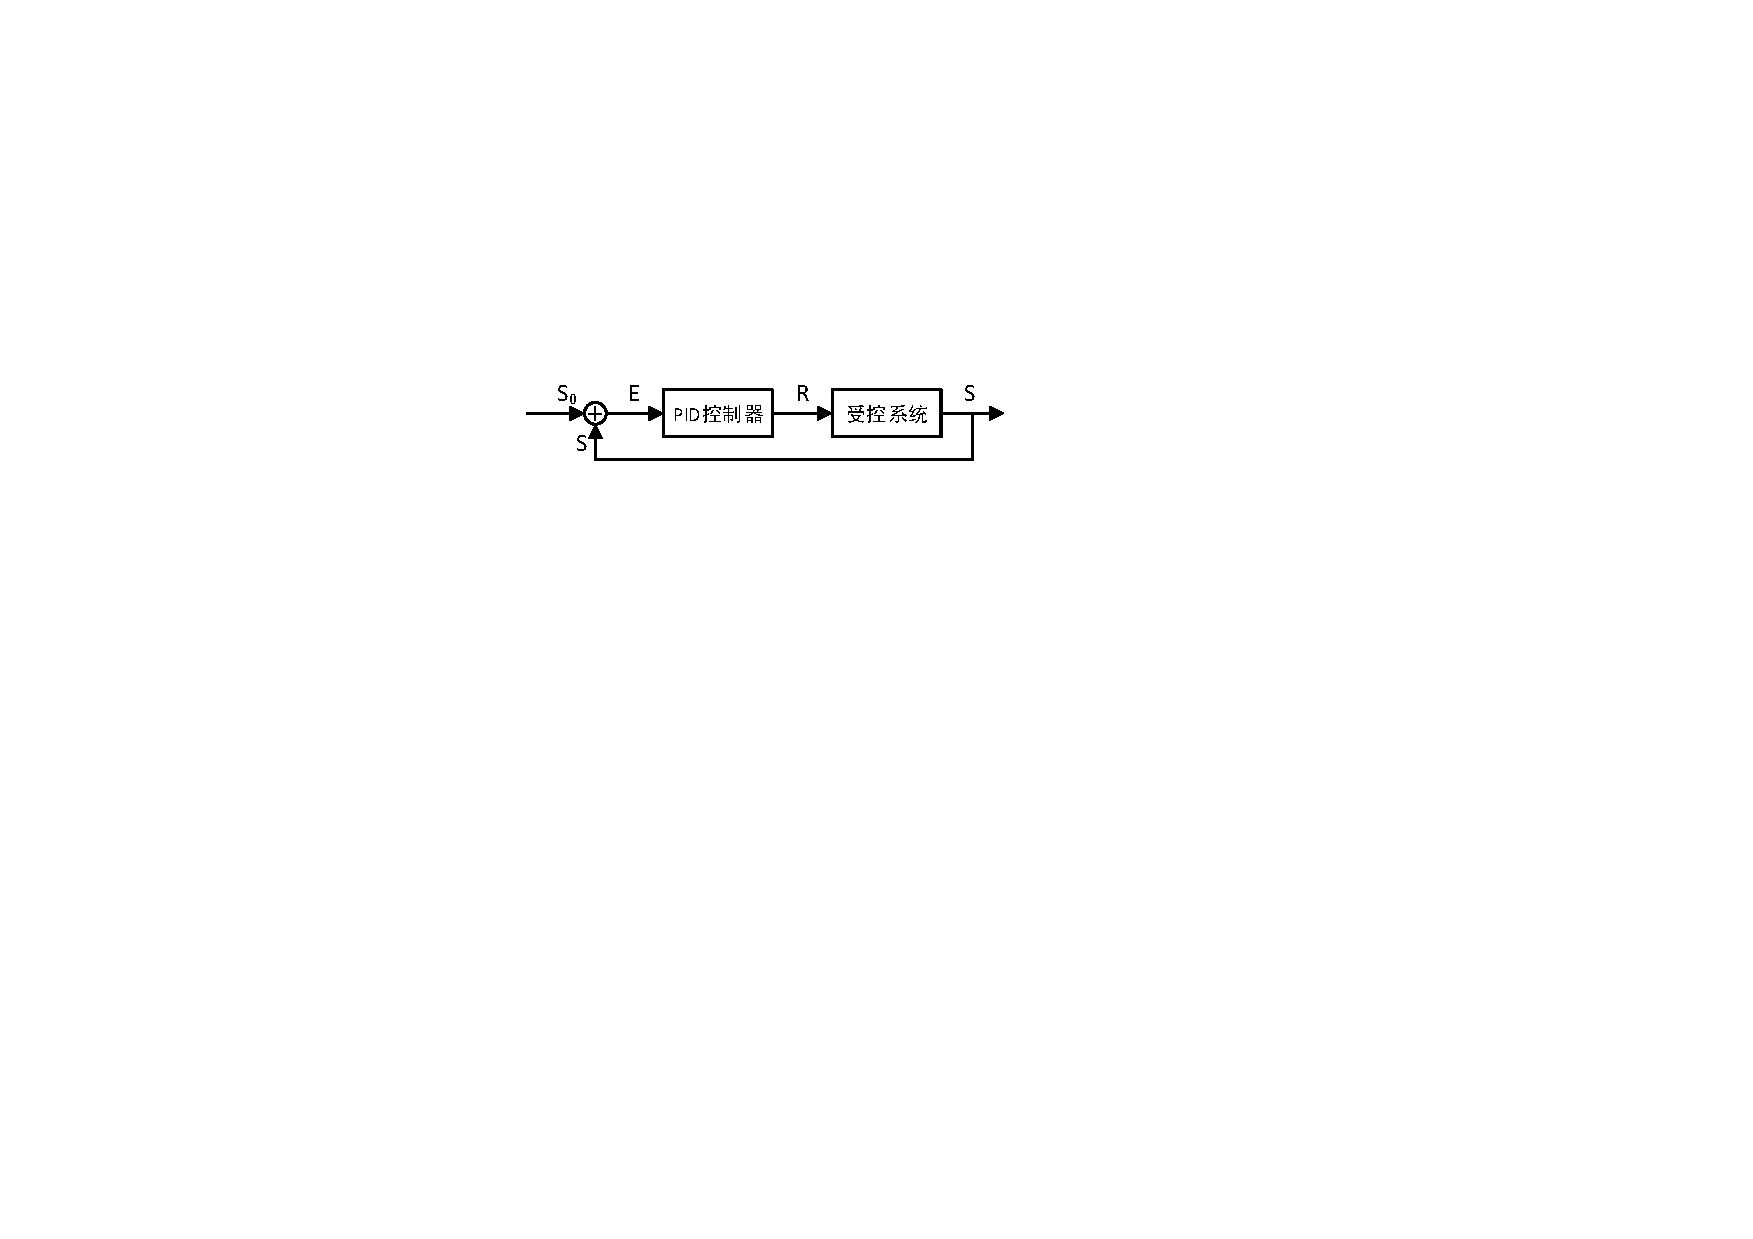
\includegraphics[width=0.6\textwidth]{intro_block_diagram.pdf}
  \caption{基本控制框图}
  \label{fig:intro_block_diagram}
\end{figure}

一种更加直接的拥塞控制方式是通过对网络建模,显式地预测网络带宽的数值。如Floyd \cite{floyd1999promoting} 等人给出的码率估算模型
\begin{equation}
  r \le \frac{1.5\sqrt{2/3} * MTU}{RTT * \sqrt{p}}
\end{equation}
其中$MTU$(Maximum transit unit)为当前网络最大传输单元,$RTT$(Round Trip Time)为数据包往返时延。与此类似的还有专为多媒体流传输设计的TFRC(TCP Friendly Rate Control) 协议 \cite{handley2003tcp},该协议兼顾了码率上升的速度,从而避免引起网络上其他采用TCP协议的数据流的``饥饿''现象。基于模型的拥塞控制算法可以看做一个闭环控制模型,以网络状态作为反馈输入,目标视频码率作为输出。而PID控制器由于其简单且良好的控制性能,在很多研究中被应用在拥塞控制模型中以提高系统表现。Wong \cite{wong2004pid} 等人给出了如图 \ref{fig:intro_block_diagram} 所示的实时视频传输基本闭环控制框图,其中系统目标状态$S_0$和系统当前状态$S_0$的差值$E$作为PID控制器的输入,控制器输入下一时刻的目标码率$R$,这一码率被设定在受控系统中,经过一定时间的运行产生下一控制时刻的系统状态$S$。
Tian \cite{tian2012towards} 等人将PID控制器应用在DASH视频直播系统中以兼顾码率控制过程中的反应速度和平滑性,也得到了较好的效果。


一直以来,传统拥塞控制算法都以丢包率作为最主要的网络拥塞信号,这往往会带来一些问题。Gettys \cite{gettys2012bufferbloat} 等人指出,由于传统网络中对于各种缓冲区的过度利用,`` 缓冲区膨胀''(bufferbloat) 的趋势变得越来越明显。过多的缓冲使得数据包的传输延迟越来越大,这使得人们重新注意到实时流媒体传输对于低延迟的需求。
很多基于模型的拥塞控制算法已经引入了传输延迟作为网络探测的信号,如TCP Vegas \cite{brakmo1995tcp} 、TCP-LP \cite{kuzmanovic2003tcp}、LEDBAT \cite{shalunov2012low}等,这有利于实时传输中对延迟的控制,然而这些算法主要利用延迟作为避免与TCP过度竞争的手段,实际应用中仍然存在延迟累积等问题。在Zhu \cite{zhu2013nada} 等人最近提出的NADA算法中,传输延迟、丢包、显示拥塞通告(explicit congestion notification,ECN)标记三种网络信息被整合为一个``等效延迟''$\widetilde{d_n}$如下
\begin{equation}
  \widetilde{d_n} = d_n + 1_n^M d_M + 1_n^L d_L
\end{equation}
其中,$d_n$为每个数据包计算出的单向传输延迟,$1_n^M$和$1_n^L$取值0或1分别对应ECN标记和丢包是否发生。$d_M$和$d_L$分别对应ECN标记和丢包事件对应的惩罚延迟时间(如$d_M=200ms$,$d_L=1s$)。在发送端根据上述``等效延迟''进行码率自适应,其码率更新公式为
\begin{equation}
  R = R_{min} + w(R_{max} - R_{min}) \frac{d_ref}{\widetilde{d_n}}
\end{equation}
其中$R_{min}$和$R_{max}$代表与视频内容和视频编码器相关的码率范围,每个视频流可以指定一个权重$w$,来获取不同比例的网络带宽。$d_ref$是认为设定的目标网络延迟。
尽管这一思路综合考虑了丢包和延迟对码率的影响,但是其整合公式和码率调整公式都比较直接,在高度动态的网络下很难取得预期的效果。

\begin{figure}[htbp]
  \centering
  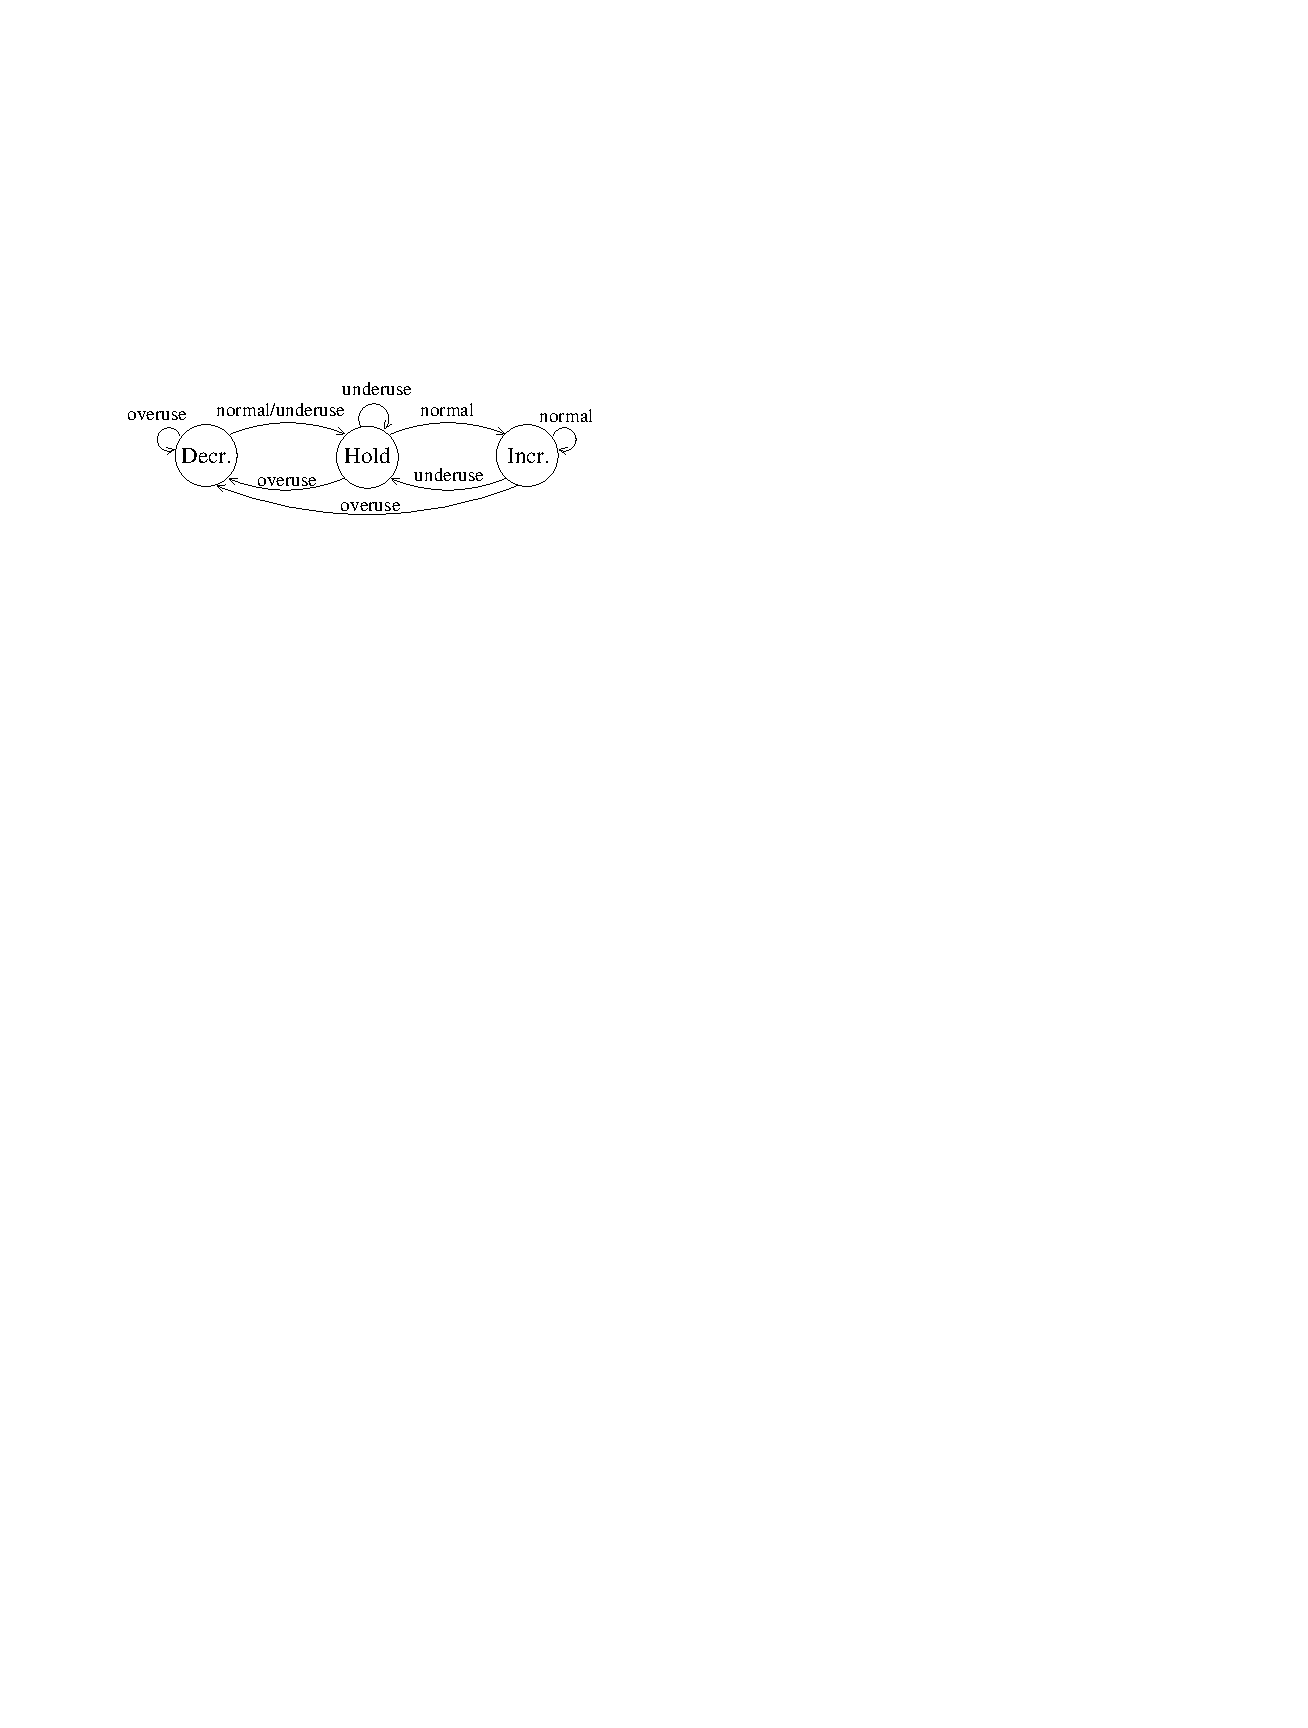
\includegraphics[width=0.7\textwidth]{gcc_state.pdf}
  \caption{WebRTC拥塞控制算法的有限状态机模型}
  \label{fig:gcc_state}
\end{figure}

\begin{figure}[htbp]
  \centering
  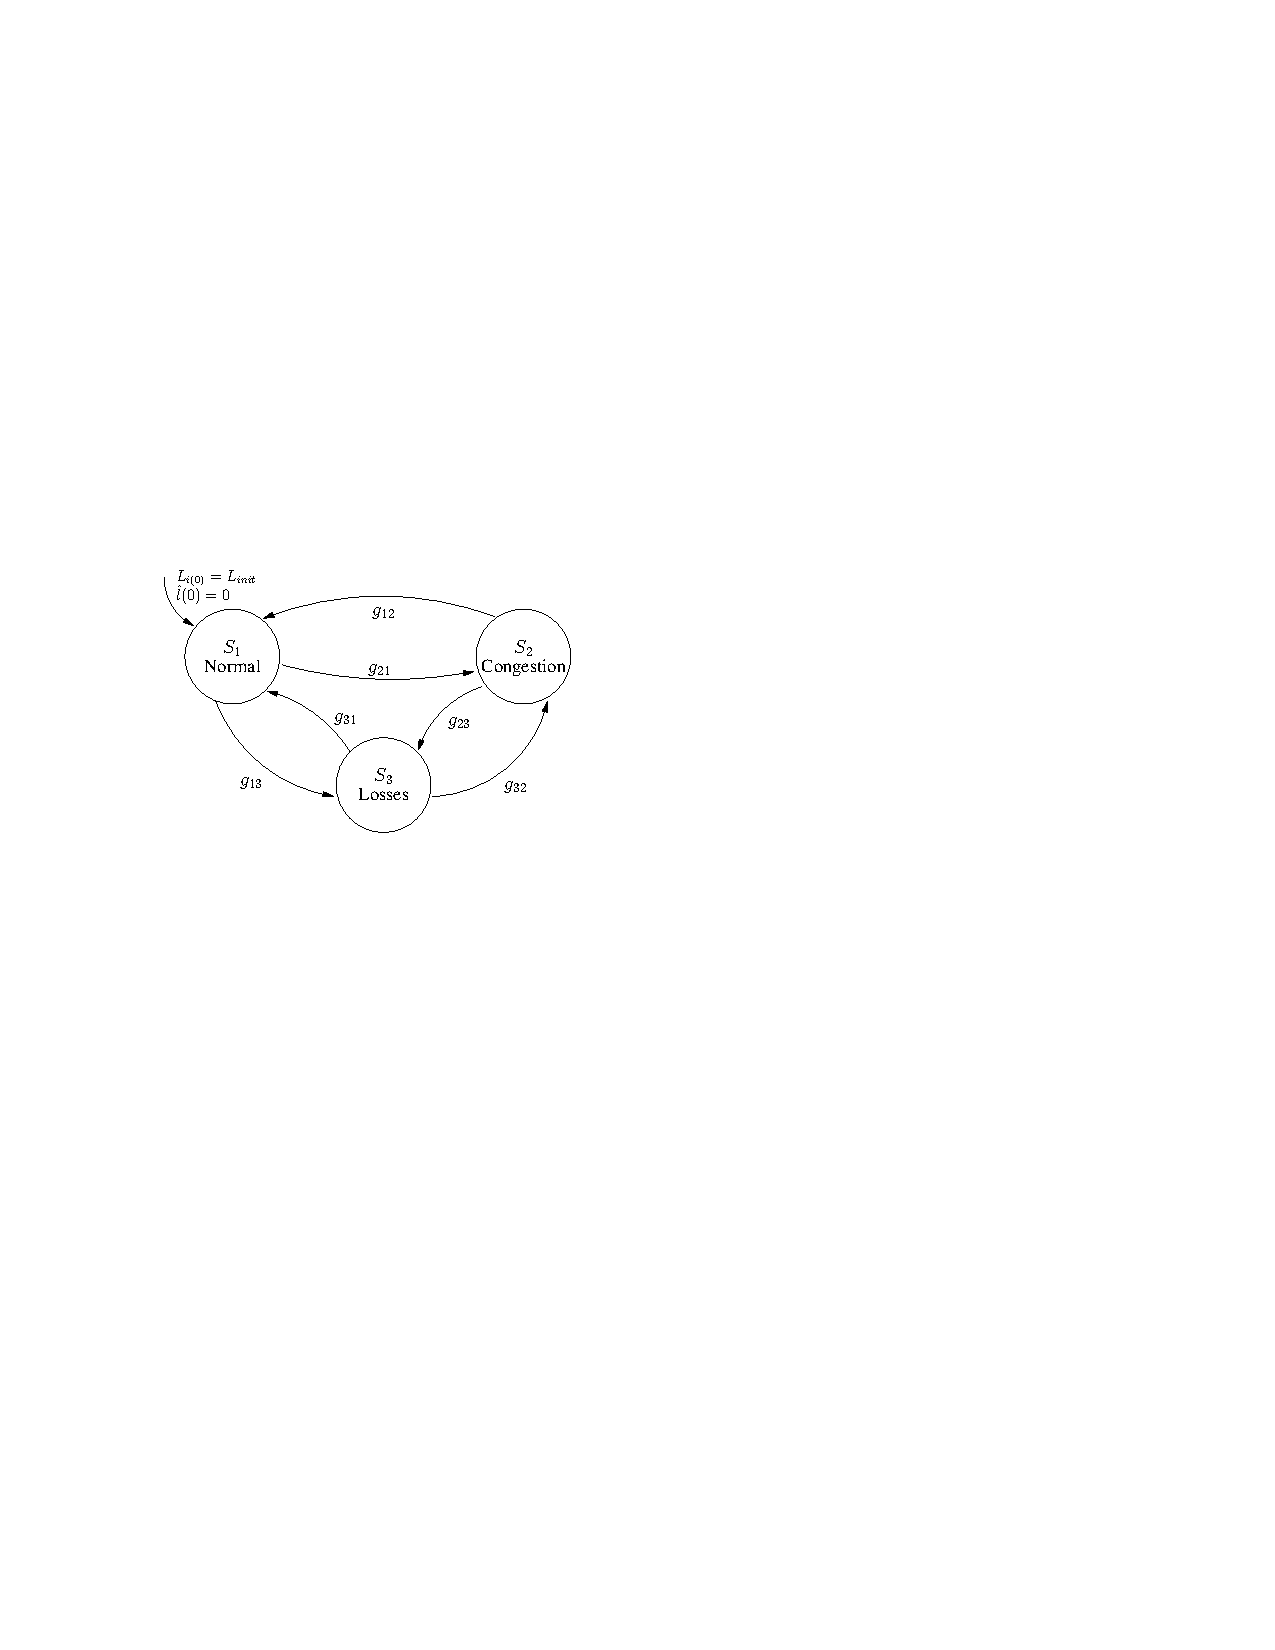
\includegraphics[width=0.5\textwidth]{skype_state.pdf}
  \caption{Skype拥塞控制算法的有限状态机模型}
  \label{fig:skype_state}
\end{figure}

以上用于实时视频的码率自适应方法都在很大程度上借鉴了传统拥塞控制算法的思想,而随着近年来互联网的发展,实时视频服务的研究在学术和工业界都获得了大量的关注。随着Skype、FaceTime、WebRTC等视频通话应用的兴起,一些应用在实际软件中的全新码率自适应算法也随之出现。De \cite{de2013experimental} 等人分析了Google在WebRTC中采用的发送、接收端混合码率自适应算法。其发送端采用基于丢包率的MIMD算法,并综合了TFRC算法
\begin{equation}
  r_t = \left\{ \begin{array}{ll}
    max\{X_t, r_{t-1}(1-0.5p)\} &   p > 0.1\\
    1.05(r_{t-1} + 1kbps)       &   p < 0.02\\
    r_{t-1}                     &   otherwise
  \end{array} \right.
\end{equation}
其中$X_t$为TFRC算法模型估算出的网络带宽。接收端采用了基于网络延迟的算法,并用图 \ref{fig:gcc_state} 所示的有限状态机描述延迟变化趋势,状态间跳转通过专门的网络探测逻辑实现。其相应码率计算公式为
\begin{equation}
  r_t = \left\{ \begin{array}{ll}
    \eta r_{t-1} &   Increase\\
    \alpha R_t   &   Decrease\\
    r_{t-1}      &   Hold
  \end{array} \right.
\end{equation}
其中$R_t$为接收端统计的当前接收速率。
LD Cicco \cite{cicco2010mathematical} 等人对Skype的研究也给出了极其相似的基于有限状态机的控制算法,其状态转移过程如图 \ref{fig:skype_state} 所示。
在开源VoIP软件Linphone \cite{website:linphone}的底层代码中,也出现了使用有限状态机对网络状态进行检测并针对不同状态应用不同码率调整策略的算法。

尽管实时多媒体流传输的码率控制问题已经获得了大量关注并在学术和工业界出现了各种算法,但目前还没有一种算法在效果方面得到广泛认同,尤其是专门针对无线网络特点进行优化的算法更是少之又少。目前互联网工程任务组(The Internet Engineering Task Force, IETF)的一个工作组RMCAT \cite{website:rmcat} 正在收集用于音视频实时传输的拥塞控制算法。这也是在我们的研究中努力解决的一个问题。


\section{实时视频流的非对称差错保护}
\label{section:fec_intro}
在网络尤其是无线网络传输过程中,由于网络拥塞、路由器转发错误、信道错误等问题不可避免地会发生丢包。而视频编码传输过程中为了压缩数据量采用的帧内和帧间压缩策略使其对数据错误十分敏感,一旦发生错误或丢包,可能对视频解码过程产生非常严重的影响,造成连续多帧的失真 \cite{stockhammer2003h}。因此我们有必要在传输过程中进行差错控制。

信道上的差错控制技术就是传统的信道编码,是为了克服信道错误而采取的必要措施。信道编码在发送端以某种确定的关联规则(约束)计算校验码元或监督码元,附在被传输的信息序列上。接收端按照既定的规则检查相应码元,如果传输过程中有信息错误或丢失,将会检测到关联信息的变化,从而实现发现错误,乃至纠正错误 \cite{陈敏2004网络实时视频传输研究, wang1998error, wang2000error} 。
基于信道编码的差错控制主要包括检错重传和前向纠错两种:
\begin{description}
    \item[检错重传(Auto Repeated Request, ARQ) \cite{soltani2009delay, schier2012optimizing}] 通过在发送数据包中添加一定冗余编码达到检错目的。接收端进行完整性检验,一旦发现丢包,则向发送端反馈重传请求,发送端重新发送数据包。此过程一直重复直到接收端收到正确的数据包。这是TCP协议中最重要的数据保障策略,然而在实时传输中并不适用。
    \item[前向纠错(Forward Error Correction, FEC) \cite{nafaa2008forward}] 通过向发送数据中添加一定量冗余数据,同时提供数据检错和纠错能力。只要错误和丢包数量不超过一定阈值,接收端就可以解码恢复所有原始数据。这一方法不需要反馈信道,比TCP实时性好 \cite{davis1996joint},因此是需要纠错能力的实时视频传输中常用的方法。
\end{description}

\begin{figure}[htbp]
  \centering
  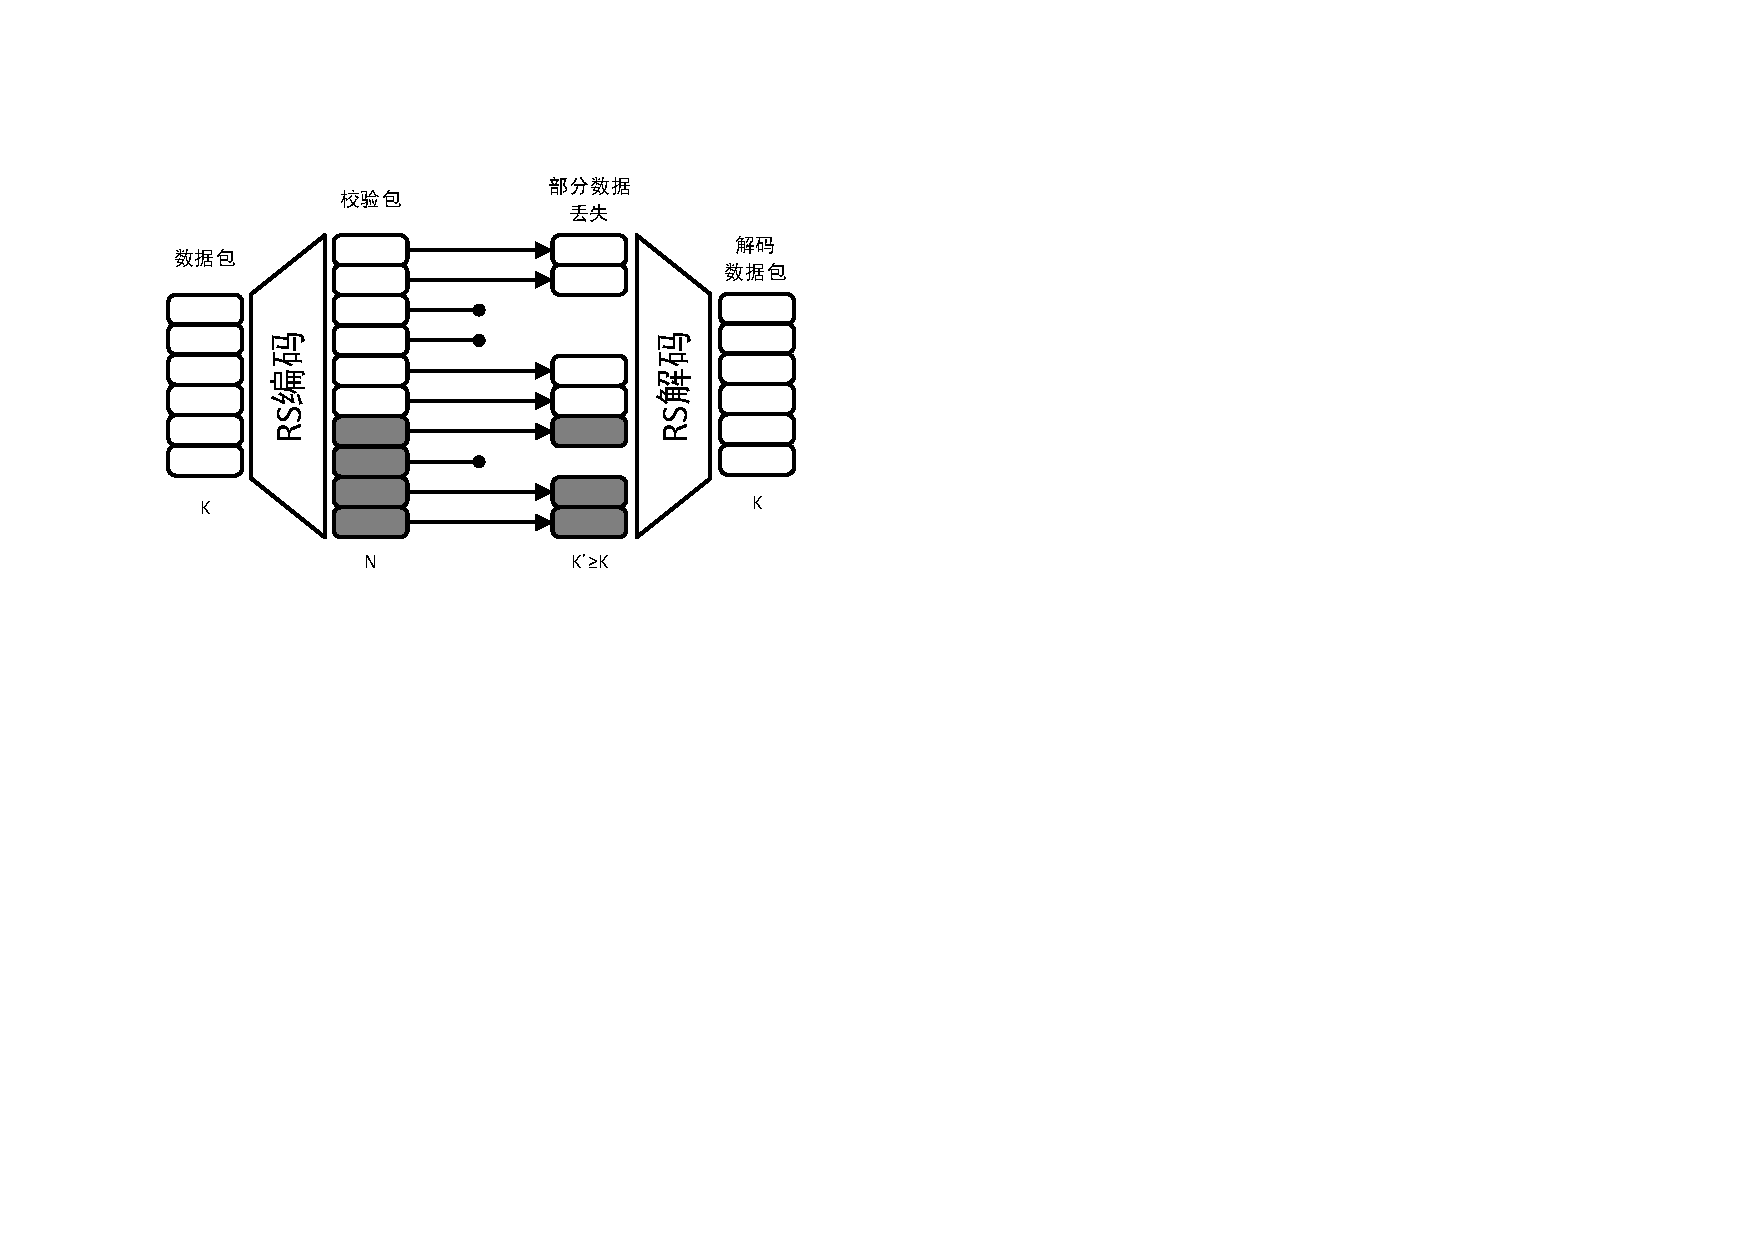
\includegraphics[width=0.7\textwidth]{RS_n_k.pdf}
  \caption{Reed-Solomon码}
  \label{fig:RS_n_k}
\end{figure}

在实时流媒体传输中,使用最多的FEC编码包括LDPC \cite{richardson2003error}和Reed Solomon(RS)编码 \cite{wicker1999reed},它们也是在RTP协议中推荐的差错保护编码方式。RS 编码是一种扩展的非二进制BCH码,在$GF(2^m)$域上进行运算。典型的RS码可以用$RS(N,K)$表示,其中$N$为编码码块长度,$K$为编码块中的信息长度,$k=N-K=2t$表示校验码的符号数,$t$表示能纠正的错误数目。另外如果错误位置已知,那么RS码可以纠正$k$个错误。RS码是一种系统码,即$K$ 个信息码元在编码之后不会发生改变。上述过程如图\ref{fig:RS_n_k}所示。

在实时视频数据流中,不同位置的数据重要性是不同的。例如在MPEG中,I 帧具有比 P 帧更重要的地位,而P帧又比B帧重要。研究 \cite{yang2005unequal, zhang2011transmission, zhang2012novel, zhou2014novel} 均表明,在视频传输中使用非对称的冗余编码能够获得更好的差错保护效果。Yang \cite{yang2005unequal} 等人提出基于失真权重的预期错误传播长度优化模型进行冗余分配。在 \cite{zhang2011transmission} 中,作者利用失真最优化的思路对冗余分配问题进行抽象表示如下:
\begin{equation}
\begin{aligned}
& \underset{\vec F}{\min}D(\vec F) =
& &  \sum_{j=1}^J D_j P_R(N_j, K_j) \\
& \text{s.t.}
& & R_C(\vec F) \le R_T - R_S \\
\end{aligned}
\end{equation}
其中$D_j$表示第$j$个BOP(Block of Pictures)的整体失真,$P_R$是$RS(N_j, K_j)$进行冗余编码后的丢包率,$R_C(\vec F)$表示冗余分配的码率限制。求解这一带约束的优化问题即可得到最优冗余分配。

然而,大部分FEC 框架的冗余保护效果依赖于较大的编码块,而包含多帧数据的编码块会引入额外的播放延迟,这对实时视频传输的效果有很大影响 \cite{wang2000error}。
在 \cite{baccaglini2008slice, bouabdallah2006dependency} 中,RS编码块包含了整个GOP中的所有数据包,因此在编解码过程中引入一个GOP的额外延迟。
Yang \cite{yang2005unequal} 等人的方法中,RS编码块中包含部分连续视频帧中的数据包(block of packets, BOP),这也引入了一个BOP的额外延迟,延迟大小取决于BOP的大小。
为了彻底解决这一问题,Thomos \cite{thomos2006robust} 等人提出一种编码块只包含单个视频帧的RS编码方法,尽管这种编码块设置不会引入任何额外延迟,然而其编码效率却大打折扣。因此,如何解决编码效率和额外延迟之间的矛盾也成为影响实时视频差错保护的关键。

\begin{figure}[htbp]
  \centering
  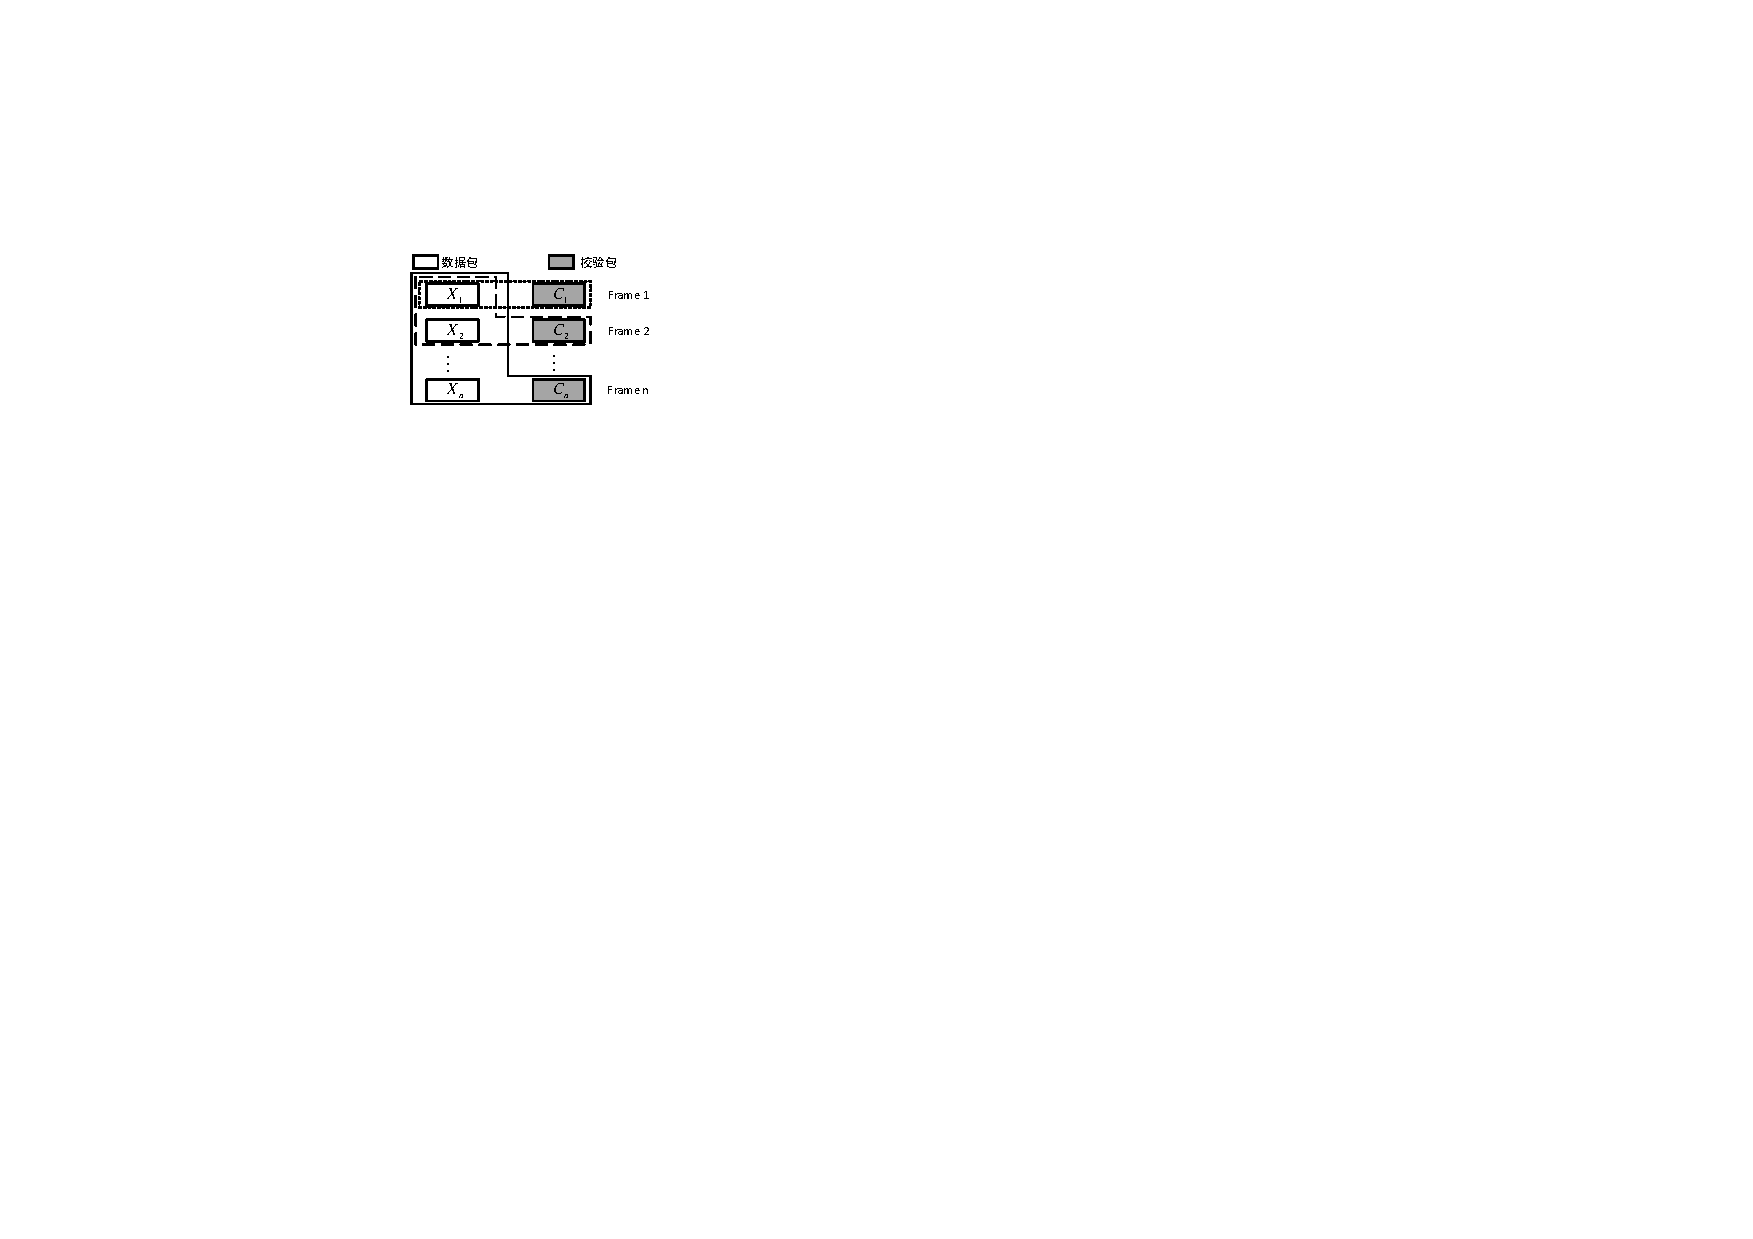
\includegraphics[width=0.6\textwidth]{ew-fec.pdf}
  \caption{扩展窗口FEC编码框架}
  \label{fig:ew_fec}
\end{figure}

随着相关研究的深入,一种能解决FEC编码块大小和额外延迟之间矛盾的扩展窗口RS编码框架(Expanding Window Reed-Solomon code, EW-RS)被提出 \cite{sejdinovic2009expanding}。 该框架编码过程如图\ref{fig:ew_fec} 所示,GOP 中第$n$个视频帧的冗余数据包$C_n$包含的编码块由第$1\le i\le n$ 帧的所有数据包组成。通过这一扩展窗口的编码块设置,编码块大小在不引入额外播放延迟的条件下得到了很大的增加。值得一提的是,这一框架还包含了非对称差错保护思想,即越靠前的数据包得到越多的保护。在 \cite{sejdinovic2009expanding, nazir2011expanding} 中,基于扩展窗口的喷泉编码模型被提出;基于扩展窗口的可伸缩视频编码(SVC)也在 \cite{vukobratovic2009scalable, hellge2011layer} 中被提出。在一项最近的工作中,Xiao \cite{xiao2013real} 等人提出了基于源数据包随机交换的Reed-Solomon 扩展窗口编码框架,该方法使用了简单有效的RS编码并通过参数随机交换解决了联立解码时的秩损失问题,具有实现简单,无额外延迟等优点。

% !Mode:: "TeX:UTF-8"
% 文字编码:UTF-8
\chapter{面向电视盒子的实时视频通话系统}
\label{chap:system}
通过前面两章介绍的视频码率自适应算法和非对称差错保护算法,我们已经较好地解决了视频通话系统中最主要的问题,并在实验中取得了良好的效果。以此为基础,我们得以完善前文提到的视频通话原型系统,基于开源视频通话软件实现一个面向安卓电视盒子和智能手机双平台、提供高清视频通话的软件,我们将其称为TVPhone(TV based Video Phone)。该软件的目标是基于未来全面覆盖的家庭Wifi 和公共Wifi 等信道,利用具有多媒体功能,提供的大屏幕、高清晰影像的电视盒子以及随时随地进行视频通话的智能手机两种平台,提供兼顾了通话效果和便利性的高清视频服务,并克服由高清视频大数据量以及无线网络质量差等对保障视频质量造成的困难。本章主要介绍 TVPhone 系统的整体设计模式、主要算法模块的实现框架和运行效果测试。

\section{背景介绍}
随着无线网络的覆盖日益广泛以及手机流量越来越廉价,人们日常生活休闲中对视频服务的需求量也越来越大,而这其中对人们生活方式改变最大的应该是通信方式从语音向信息量更丰富的视频通话转变。目前提供视频通话的应用如FaceTime、QQ、微信视频、Skype、环聊等使用率越来越高,一系列以此为基础的多媒体软件也快速涌现。

在底层传输方面,绝大部分实时视频服务都采用了RTP(Real-time Transport Protocol)实时传输协议。该协议提供了在互联网上传输实时数据(音频、视频等)所需要的基本功能,如时间戳同步、数据排序等。但该协议没有提供数据保护或传输质量保障功能,因此传输中一般还使用RTCP(Real-time Transport Control Protocol)用于传输质量监测、反馈等功能,从而实现基本的链路控制和数据保护。RTCP协议定时向发送方反馈当前网络的延迟、丢包率、网络抖动等网络基本信息,在发送端结合具体的码率自适应算法进行码率控制。在目前的视频通话应用中,主要使用了基于状态机的自适应算法,结合工程师的经验添加复杂的控制逻辑进行效果优化,而这一过程是没有理论分析支持的。另一方面,由于RTP协议不支持冗余保护,目前很多视频通话服务都没有丢包恢复功能,更不用说对冗余分配的优化,因此在信道质量较差的网络中往往播放效果很差。这也是我们前面两章的算法以及系统实现中主要解决的问题。

在本研究中,我们希望通过重新实现视频通话系统的底层传输模块,一方面利用我们的码率自适应算法,实现视频通话过程中的延迟可控,并通过理论分析有针对地提升码率调整的效果;另一方面,增加一个独立的FEC冗余保护模块,并结合冗余分配优化方案,在高丢包网络下保证稳定的视频质量。考虑到实时视频传输过程中涉及到的视频采集、编解码、播放以及传输过程中的连接建立、维护等功能实现起来都十分复杂并且已经有成熟的实现,而且这部分也不是本研究中关注的重点,因此我们选择了比较成熟的开源视频通话软件Linphone\cite{website:linphone}作为算法模块实现的基础。


    \subsection{Linphone项目框架}
    
    \begin{figure}[htbp]
      \centering
      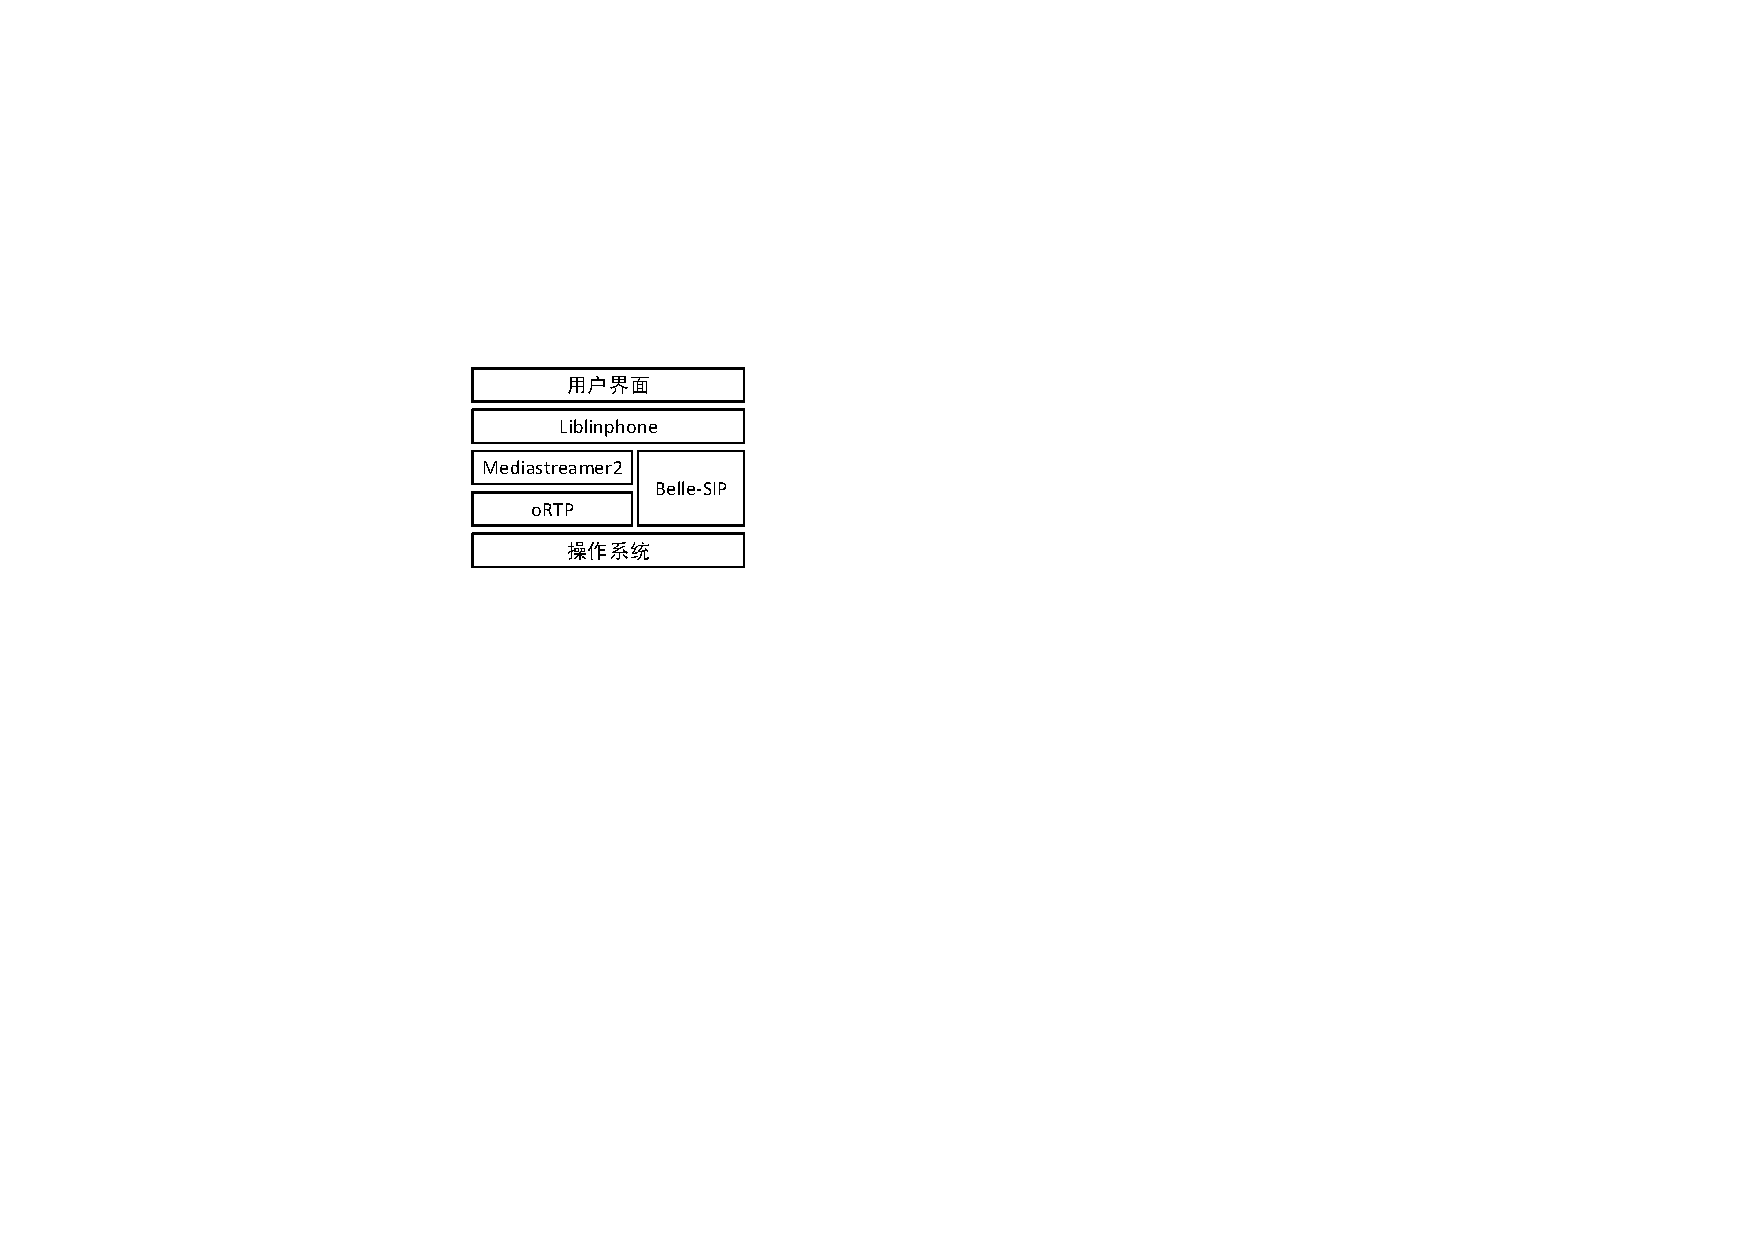
\includegraphics[width=0.4\textwidth]{sys_linphone_arch.pdf}
      \caption{Liblinphone系统框架}
      \label{fig:sys_linphone_arch}
    \end{figure}
    
    Linphone是一个开源视频通话软件,支持包括Windows、MAC OSX、Linux、Android、iOS等平台。如图 \ref{fig:sys_linphone_arch} 所示,Linphone核心功能位于上层用户界面和底层操作系统之间,其用户界面可以为不同平台和设备提供专门的界面支持,底层操作系统则提供了音视频驱动、系统函数调用等功能。而Liblinphone是其最主要的功能模块,封装了进行视频通话需要的所有功能,Liblinphone还依赖于以下三个功能模块:
    \begin{itemize}
        \item Mediastreamer2:流媒体处理,包括音、视频的采集、编解码等功能
        \item oRTP:负责流媒体传输,RTP和RTCP协议的具体实现
        \item belle-sip:提供SIP协议支持的库
    \end{itemize}
    以上所有Liblinphone的内容都采用纯C代码实现。在TVPhone的开发中,我们主要关注包含视频处理的Mediastreamer2模块和负责视频传输的oRTP模块。

    \begin{figure}[htbp]
      \centering
      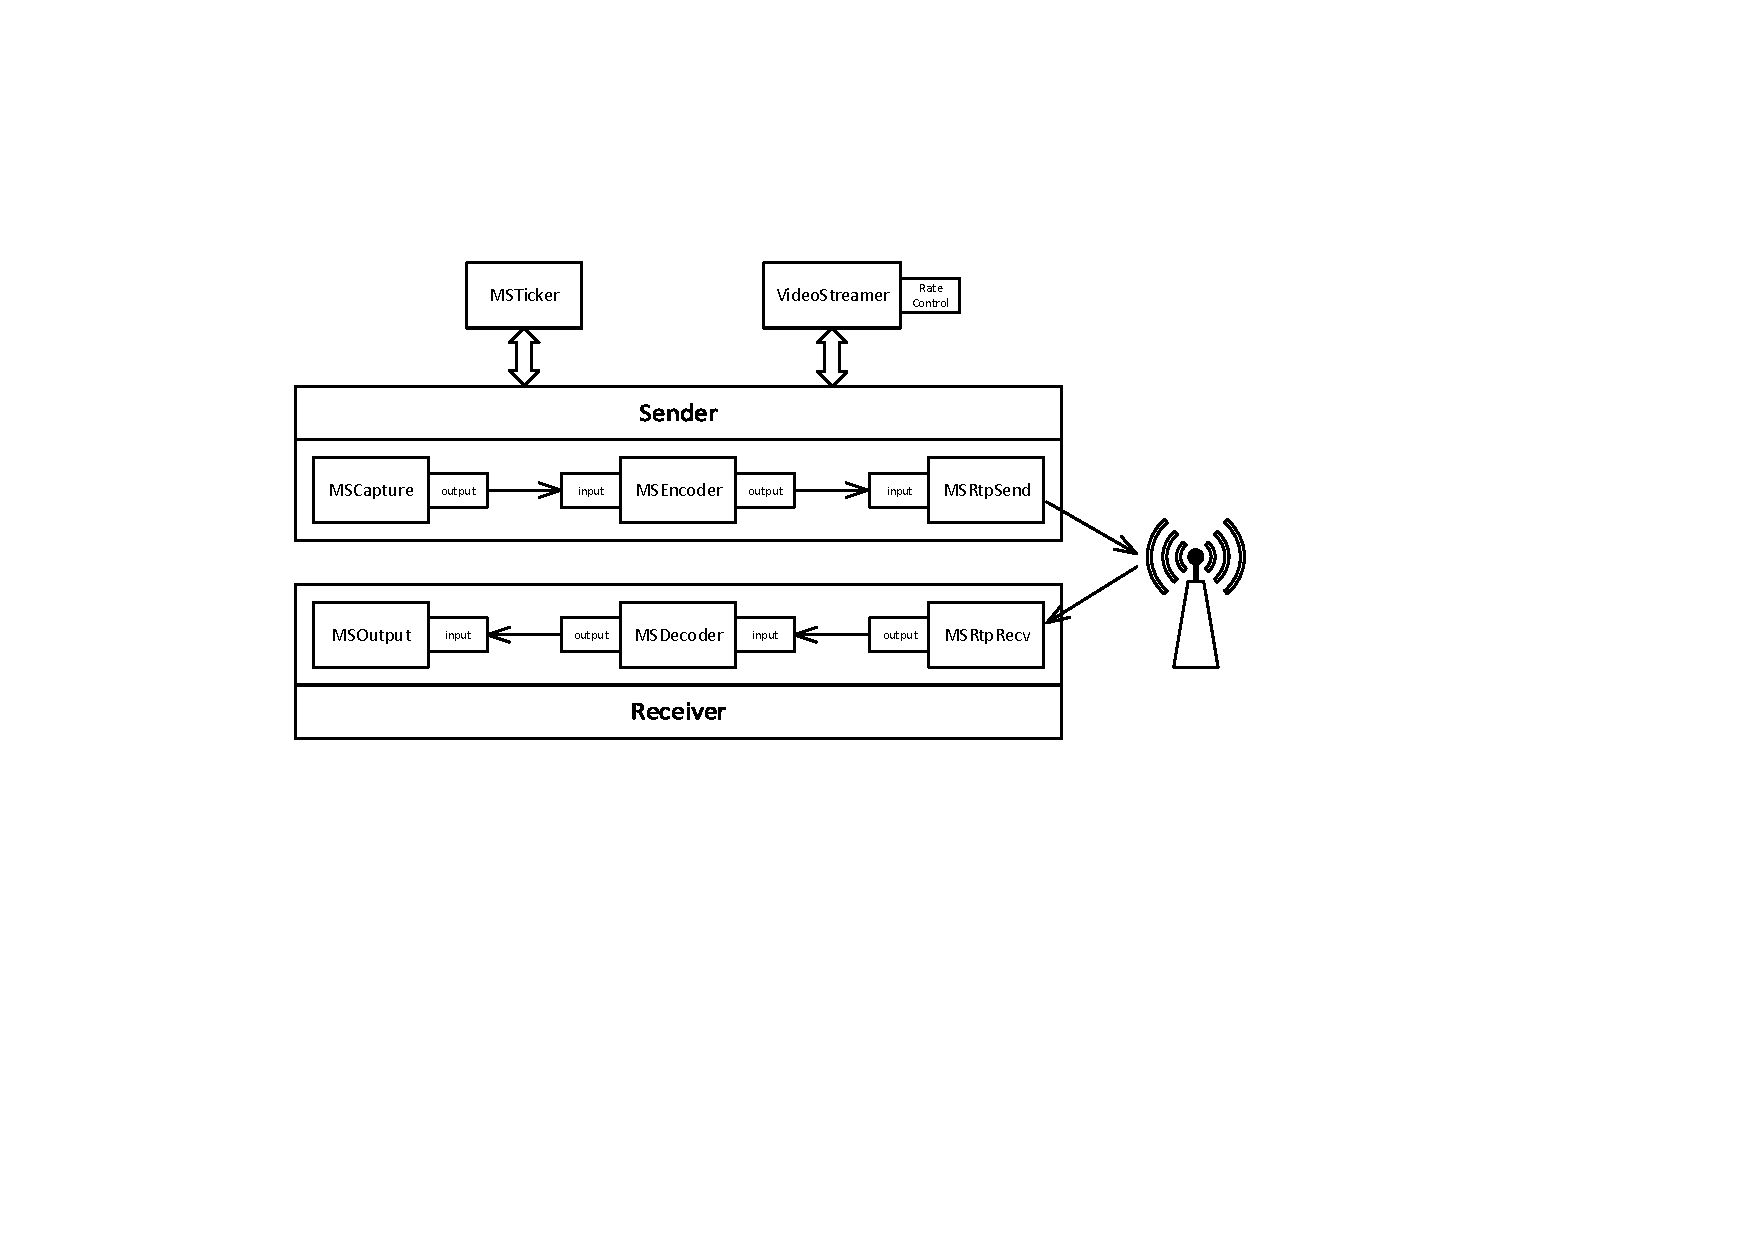
\includegraphics[width=0.9\textwidth]{linphone1.pdf}
      \caption{Liblinphone系统框架}
      \label{fig:linphone1}
    \end{figure}

    Liblinphone采用了模块化的设计模式,每一个功能模块实现为一个Filter数据结构,完成一项具体操作(视频采集、编码、封装等)。每个Filter都实现了统一的输入和输出接口,利用函数指针将需要的Filter组合起来即可完成整个服务过程,完成视频通话需要的基本Filter组合框架如图 \ref{fig:linphone1} 所示。在发送端,MSCapture完成视频数据的采集,原始视频数据进入MSEncoder进行压缩编码,编码后的数据在MSRtpSend完成RTP协议封装并通过网络链接向接收端发送。接收端MSRtpRecv接收到网络数据,对RTP 数据包进行拆包得到视频数据,经过MSDecoder解码即可通过MSOutput播放视频画面。另外VideoStreamer是一个单独启动的Filter,完成网络信息的收集和反馈并以此为基础进行码率控制。注意到图中VideoStreamer附带的码率控制(Rate Control)模块是Linphone已经实现的码率控制协议,实现了一套较复杂的基于状态机的码率控制,但其表现尚有较大提升空间。另外,上述过程通过在独立线程中启动的MSTicker 进行调度。以上所有Filter 都只定义了输入和输出信息的格式,因此可以根据需要随意替换其具体实现,如MSEncoder 可以实现为VP8 或H.264 等不同的视频编码格式。

    \subsection{RTP与RTCP传输协议}
    RTP(实时传输协议),顾名思义就是用来传输实时数据的,它作为因特网标准在RFC 3550\cite{jacobson2003rtp}中有详细说明。它为实时音、视频传输提供实时的传输服务,其中包括载荷类型标记、序列编号、时间戳和送达检测等。接收端可以利用RTP包头中的序列号和时间戳进行数据包的重排序和丢包检测。大部分应用将RTP建立在UDP协议之上,以利用其数据包校验、多地址发送等特性。需要注意的是,RTP本身并不提供任何机制保障数据包按时到达或其他传输质量保证,数据包可能发生丢包或乱序到达。

    RTCP为RTP数据流提供信道外控制。RTCP本身并不传输数据,而是定期在会话参加者之间传输控制数据。RTCP的主要功能是为RTP所提供的服务质量提供反馈。RTCP收集相关媒体连接的统计信息,如传输字节数,传输分组数,丢失分组数,jitter,单向和双向网络延迟等等,网络应用程序即可利用RTCP的统计信息来控制传输的品质,比如当网络带宽高负载时限制信息流量或改用压缩比较小的编解码器设置。

    Linphone中的oRTP模块就是对上述RTP和RTCP协议的封装,并实现了数据包的丢包检测,重排序等功能。我们的码率自适应算法也主要使用了RTCP协议所携带的网络信息进行码率控制。

\section{系统设计}


\subsection{设计框架}

\begin{figure}[htbp]
  \centering
  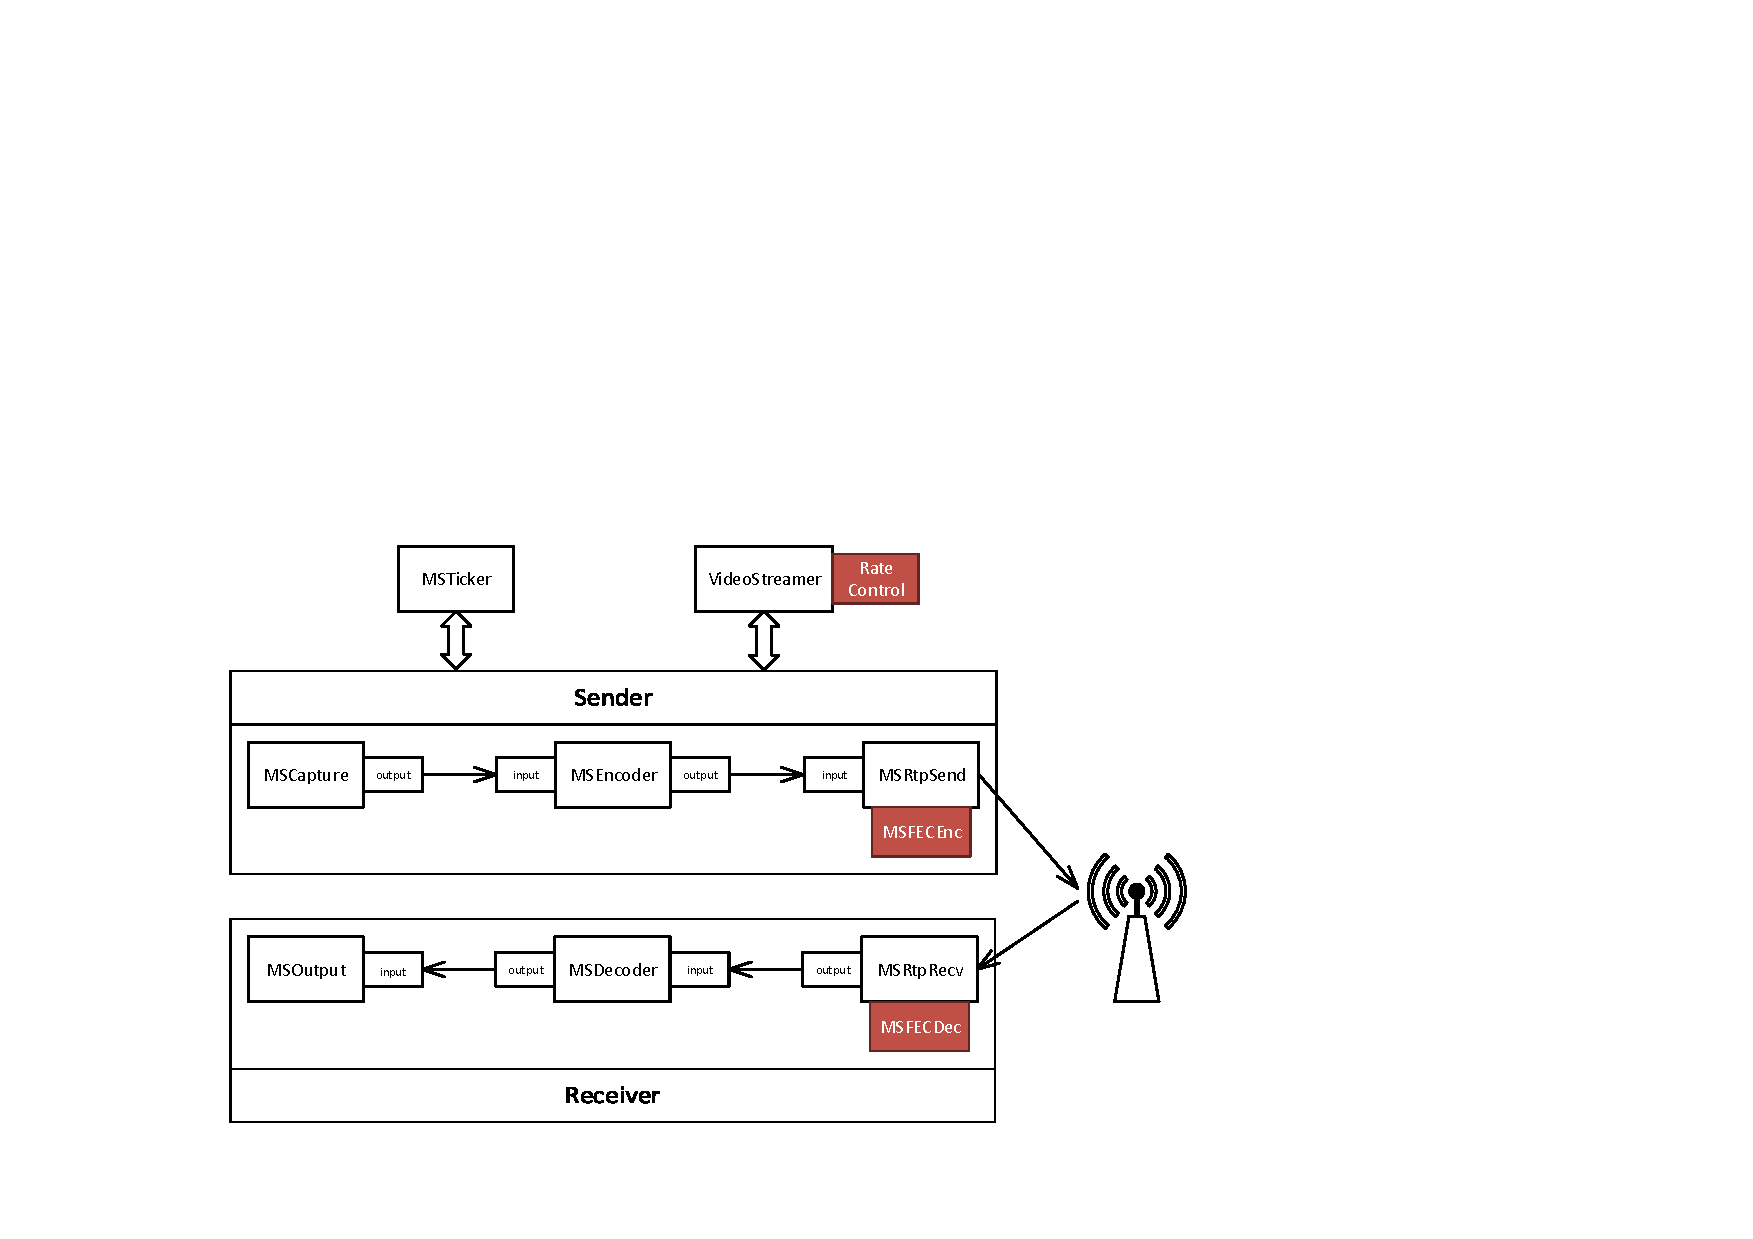
\includegraphics[width=0.95\textwidth]{linphone2.pdf}
  \caption{Liblinphone改进系统框架}
  \label{fig:linphone2}
\end{figure}

如上所述,在TVPhone系统中,我们主要关注码率自适应和差错保护两个模块的实现和优化,对于视频采集播放、编解码、RTP封装等操作直接沿用Linphone中的代码。基于上述Filter 设计模式,我们设计出如图\ref{fig:linphone2}所示的改进系统框架。

一方面,我们沿用Linphone原有的码率控制框架,进行一些必要的改进之后替换了我们的码率自适应算法。我们在接收端通过一个网络探测模块获取网络状况信息(单向延迟、丢包率等),码率自适应模块以当前网络状况为输入,经过计算输出相应的最优视频码率并按照固定时间间隔通过RTCP协议反馈给发送端,发送端调用底层视频编码器接口改变输出视频的码率。

另一方面,根据原始LibLinphone 的MSRtpSend和MSRtpRecv模块设计,底层进行RTP包封装后直接发送数据到UDP网络层。为了实现冗余保护功能,我们在MSRtpSend 的输出端和网络链路之间增加了一个FEC 冗余编码模块 MSFECEnc,以及在MSRtpRecv 处理网络数据包之前增加了一个FEC 解码模块 MSFECDec,这两个模块分别作为RTP模块的附属功能单元进行FEC编解码操作。这样,所有发送到网络的RTP 数据包都添加了FEC 冗余数据,只要丢包数量低于FEC 解码的阈值,即可避免视频失真。


\subsection{码率自适应模块}
码率自适应是实时视频传输过程中最核心的控制模块,保证了视频通话服务在任何网络下都能合理利用当前可用带宽并获得相对较好的传输效果。我们设计的TVPhone码率自适应模块主要采用了第\ref{chap:rate}章提出的延迟优化的实时视频码率自适应算法,针对实时视频的需求,以排队延迟为主要参考信号,以低延迟和稳定高效的带宽利用为目标进行视频码率控制。

    \subsubsection{上层接口描述}
    \begin{lstlisting}[language=C]
int rc_process_rtcp(MSQosAnalyzer *objbase, mblk_t *rtcp);
    \end{lstlisting}

    码率自适应模块对上层提供的接口只有一个函数 \lstinline!rc_process_rtcp!,该函数的主要功能是网络状态信息收集、延迟优化的码率自适应计算和定时向发送端反馈等。其输入 \lstinline!objbase! 指向码率自适应模块的内存实体,记录码率自适应算法的设置、需要保存的历史状态等; \lstinline!rtcp! 指向接收到的RTCP包,通过解析RTCP 包可以得到单向延迟、网络丢包率等码率自适应算法需要的信息。输出为代表函数执行状态的整数代码。该函数在系统收到携带网络状态信息的RTCP包时被调用。

    上述接口的内部实现逻辑将在下节介绍。

    \subsubsection{模块设计框架}
    \begin{figure}[htbp]
      \centering
      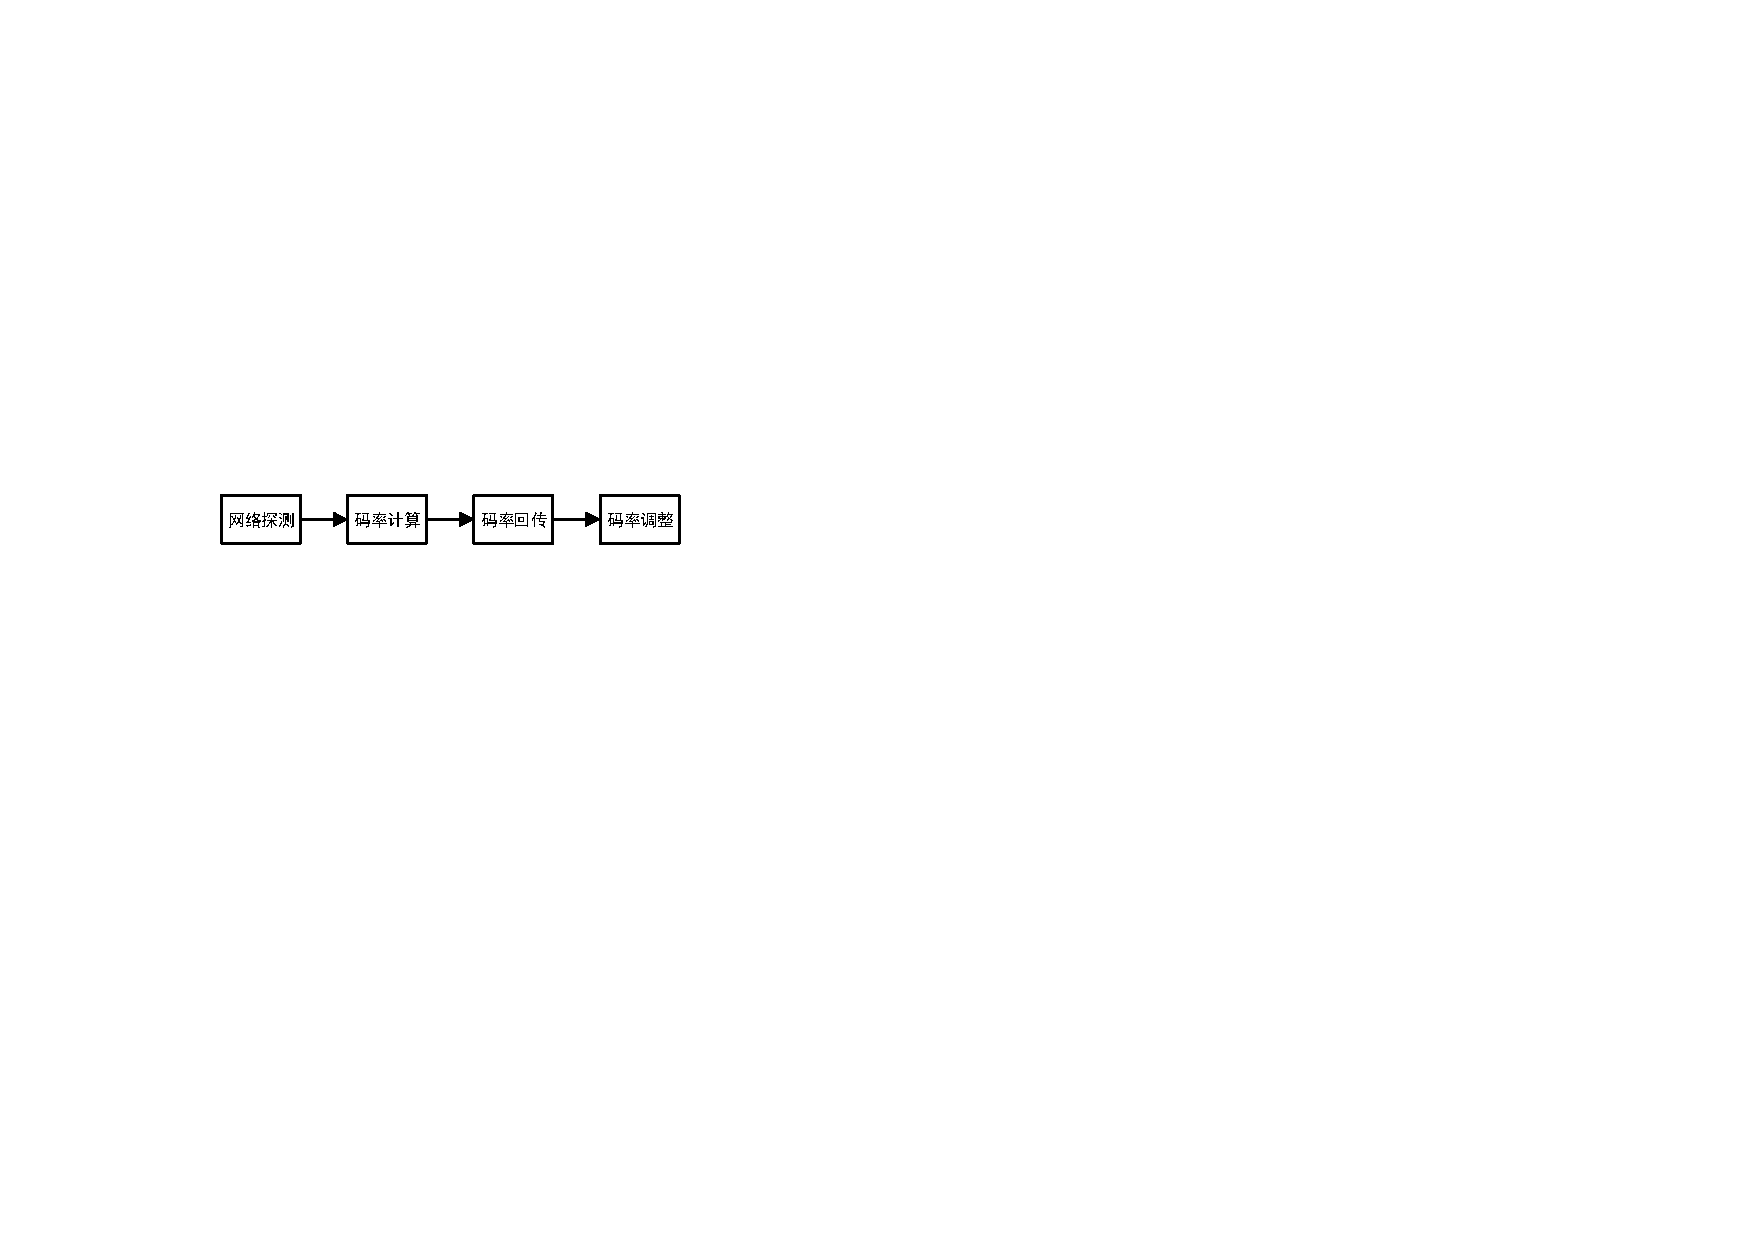
\includegraphics[width=0.8\textwidth]{rate_control.pdf}
      \caption{码率自适应模块设计框架}
      \label{fig:rate_control_arch}
    \end{figure}

    尽管上层接口较简单,但函数内部需要完成的操作并不少。如图\ref{fig:rate_control_arch}所示,码率自适应模块的主要功能单元包括网络探测、码率计算、码率回传和码率调整四部分。

    ``网络探测''单元为码率自适应算法提供必要的网络运行状态参数,在我们的算法中主要用到排队延迟。在第\ref{chap:qd_calc}节中,我们已经给出了利用单向延迟计算排队延迟的方法,因此网络探测模块需要提供单向延迟的探测。为了探测网络的延迟,发送端每隔100ms发送一个RTCP探测包并标记发送时刻的时间戳,接收端收到该RTCP包即可利用发送和接收的时间差计算单向延迟、最小单向延迟,进而根据式\ref{eq:qd}计算排队延迟。另外,网络探测模块还根据收到RTP包的序列号统计网络丢包率,以供极端情况下的码率调整和差错保护。

    ``码率计算''单元是运行在视频接收端的功能单元,其根据网络探测输入的延迟和丢包率信息,套用第\ref{chap:rate}章算法计算目标码率并提交给``码率回传''单元反馈给发送端。将码率计算单元设置在接收端主要有两点考虑:
    \begin{enumerate}
        \item 视频传输过程中,排队延迟、丢包率等网络参数的统计都在接收端完成,回传目标视频码率的通信量明显低于回传全部网络参数所需要的通信量。
        \item 系统运行过程中,接收端网络参数的采集频率可以很高。码率计算在接收端进行,更频繁地计算目标码率值,并根据这一值的变化情况动态地选择更加合理的回传频率,以优化系统反应速度和带宽占用。
    \end{enumerate}
    视频码率的调整速率对视频通话系统的很多方面都有影响。如果码率调整间隔太大,会造成网络拥塞状况得不到及时解决,出现较大的延迟波动;单次调整变化过大,对用户体验造成一定影响。而如果码率调整太频繁,会造成视频编码器负载增大;回传次数增多,网络负载增加等问题。通过实验测试,我们选择了500ms作为码率回传单元回传码率的默认时间间隔。另外如果两次计算的目标码率变化超过一定阈值,则会立刻发送该目标码率以避免网络拥塞。

    码率调整单元直接调用视频编码器Filter提供的接口进行设置,由具体的VP8、H.264等编码器实现视频输出码率的控制。需要注意的是,大部分视频编码器并不能完全将输出码率固定在一个准确的值,而是会在一定范围内波动并尽量使平均码率接近目标值。这一点也给实时视频的码率自适应策略带来一定的困难,而我们基于控制论的系统优化在应对这种系统误差时具有很好的效果。


\subsection{差错保护模块}
差错保护是视频通话系统的可选模块,以增加带宽占用为代价提供一定的丢包恢复能力。在无线网络场景下,现有技术已经实现了非常高的峰值带宽,然而由于传输信道的局限,仍然存在一定的丢包情况。因此无线网络下应用差错保护成为一种性价比很高的提升视频通话效果的方案。基于无线网络通信的需求,我们在TVPhone系统中添加了一个独立的差错保护模块,并用第\ref{chap:fec}章提出的非对称差错保护算法对保护效果进行了优化。该差错保护模块的设计框架如图\ref{fig:fec_arch}所示。

    \subsubsection{上层接口描述}
    差错保护模块提供FEC编解码相关的接口供oRTP模块调用,其主要接口如下:
    \begin{lstlisting}[language=C]
int fec_set_rate(MSFecDriver *obj, int block_size, int fec_rate);
int fec_outgoing_rtp(MSFecDriver *obj, mblk_t *rtp);
int fec_incoming_rtp(MSFecDriver *obj, mblk_t *rtp);
int fec_incoming_rtcp(MSFecDriver *obj, mblk_t *rtcp);
    \end{lstlisting}

    其中 \lstinline!fec_set_rate! 可以动态调整差错保护的平均冗余率,在系统初始化时调用,也可以在系统运行中根据网络状态调用该函数动态修改冗余率。当发送端 MSRtpSend 模块准备发送RTP包时,首先调用 \lstinline!fec_outgoing_rtp! 对RTP包进行缓存,并在恰当的时机进行FEC编码和FEC冗余数据包发送。 当接收端 MSRtpRecv 模块收到RTP包或携带冗余数据的RTCP 数据包时,分别调用 \lstinline!fec_incoming_rtp! 和 \lstinline!fec_incoming_rtcp! 进行数据缓存,并在恰当的时机进行FEC解码并恢复丢失的RTP 数据包。
    
    上述接口的内部实现逻辑将在下节介绍。

    \subsubsection{模块设计框架}
    \begin{figure}[htbp]
      \centering
      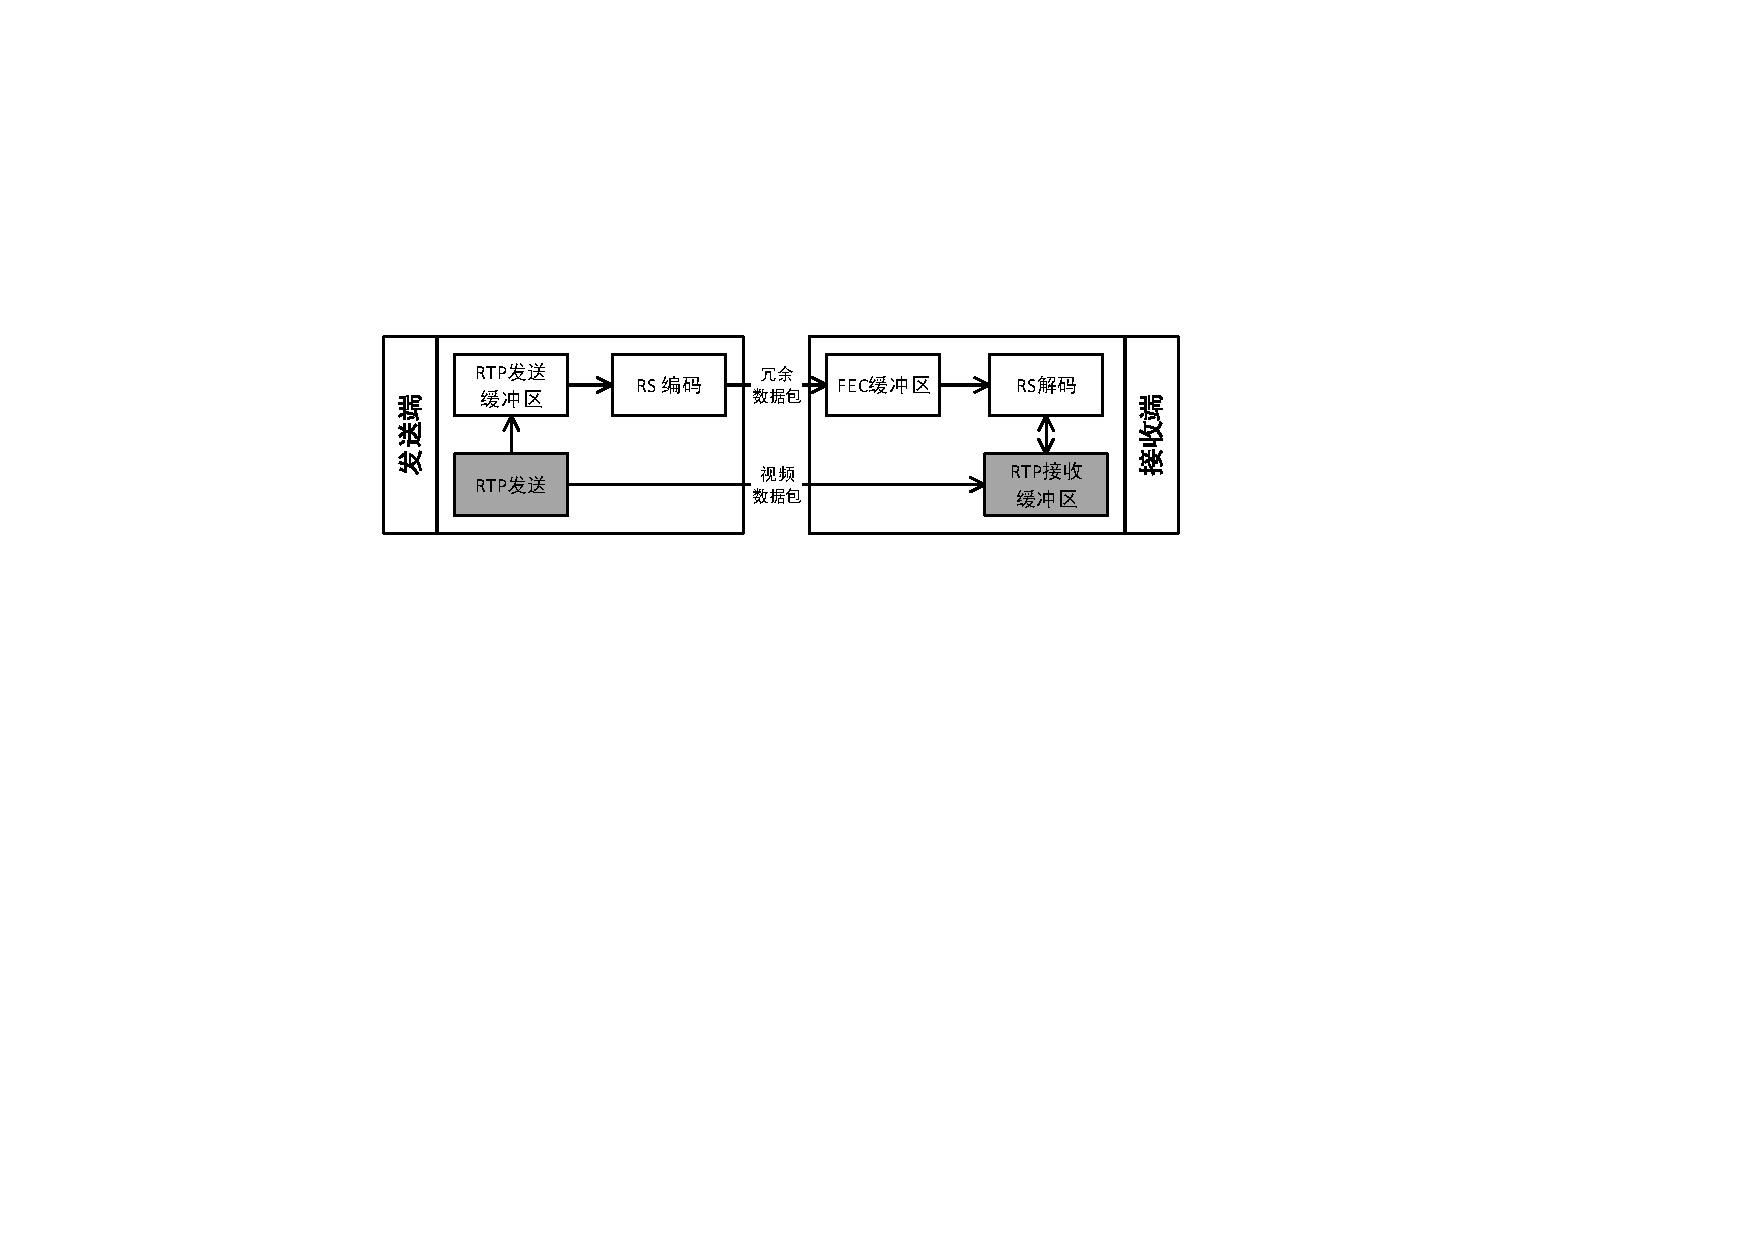
\includegraphics[width=1\textwidth]{fec.pdf}
      \caption{差错保护模块设计框架}
      \label{fig:fec_arch}
    \end{figure}

    图\ref{fig:fec_arch}中灰色单元为Liblinphone中的原生功能单元\footnotecircle{其中接收端``RTP缓冲区''单元进行了一些修改以适应扩展窗口编码要求},均实现于oRTP 中,完成RTP 协议的部分功能。具体来说,底层视频编码器产生的数据经过oRTP 的封装形成RTP 包,通过``RTP发送''单元经UDP等网络层到达接收端。在负责接收的oRTP部分维护了一个``RTP接收缓冲区'',用于缓存还未用于视频解码的RTP 包,并根据时间戳对RTP 包进行排序。当然由于实时视频传输的播放延迟非常小,数据包到达后很快就需要进行解码播放,这个RTP 缓冲区内通常只缓存了很少的数据包。

    根据第\ref{chap:fec}章的描述,我们在差错保护模块采用了实现简单且比较成熟的Reed-Solomon编码(RS编码),我们选择了Github上的一个开源Reed-Solomon编码库longhair\cite{website:longhair} 作为底层编码单元。RS编码具有$RS(N,K)$编码格式,即每个编码块对$K$个RTP包进行冗余编码生成$N-K$个FEC校验包,在接收端只要接收到该编码块中的任意$K$个包,就能通过对编码块的解码完全恢复丢失的RTP包。因此在我们的差错保护模块中,发送端需要对待编码的编码块中的RTP包进行缓存,接收端则需要对接收到的RTP包和校验包进行缓存以备解码。因此在差错保护模块中包含了发送端的``RTP发送缓冲区''以及接收端的``RTP接收缓冲区''和``FEC缓冲区''共三个缓冲区。

    发送端的``RS编码''和接收端的``RS解码''单元分别完成RS编码和解码过程。其中RS编码的输入为``RTP发送缓冲区''中的RTP包,编码结束后得到的冗余包经过RTCP协议发送到接收端。接收端以``RTP接收缓冲区''中的RTP包和``FEC缓冲区''中的校验包为输入,如果发现丢包并且满足$RS(N,K)$的解码条件,则进行解码恢复丢失的RTP包。这些恢复的RTP包也被放入``RTP接收缓冲区'',从而进入正常的视频解码流程,完成数据包的恢复。在RS编码过程中,还涉及到编码块的组织、冗余分配优化、编解码效果优化等实现细节,将在下节详细说明。

    \subsubsection{扩展窗口RS编解码实现}
    \begin{figure}[htbp]
      \centering
      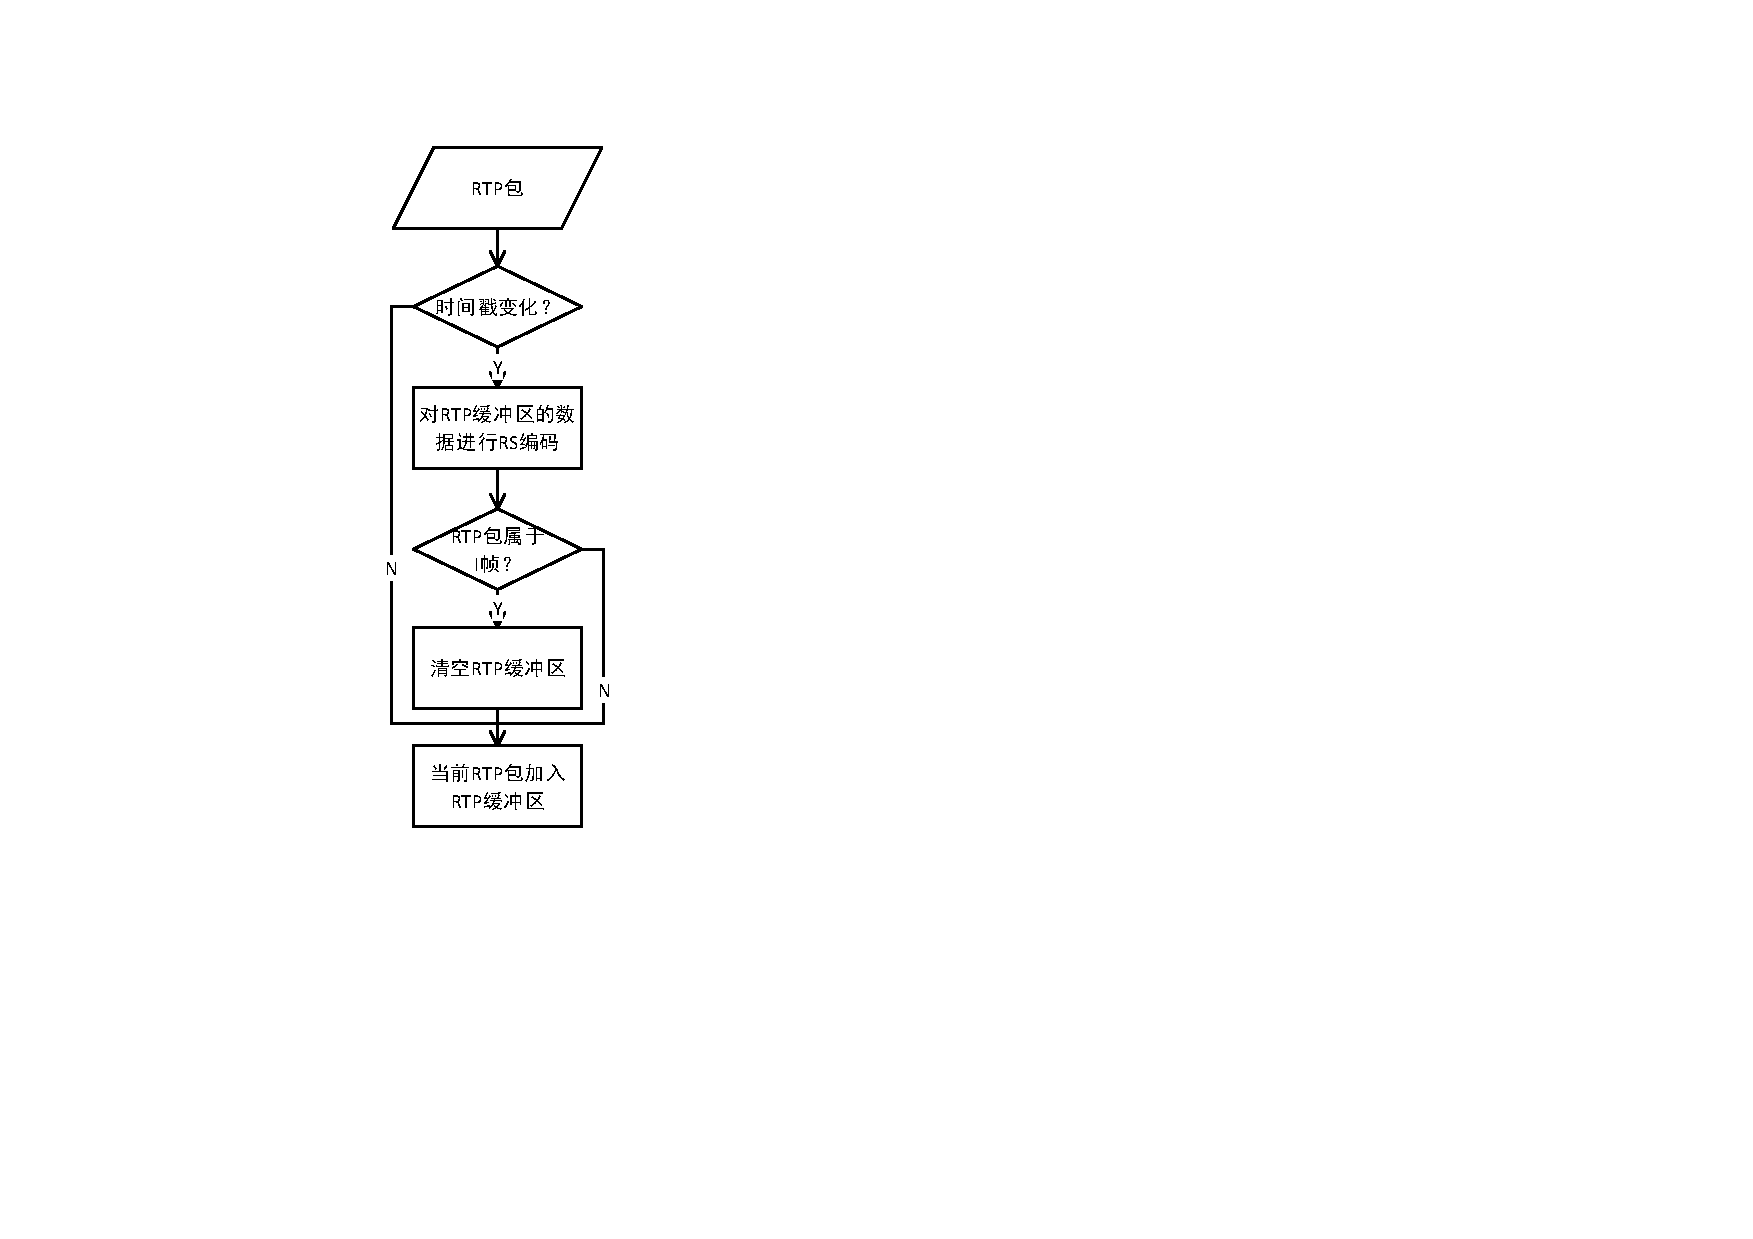
\includegraphics[width=0.25\textwidth]{fec_enc_seq.pdf}
      \caption{扩展窗口RS编码流程图}
      \label{fig:fec_enc_seq}
    \end{figure}

    由于我们的差错保护模块采用了基于扩展窗口的RS编码框架,在发送端RTP缓冲区的使用上与传统FEC编码过程有一定差别,编码过程也需要进行修改,发送端编码的流程图如图 \ref{fig:fec_enc_seq} 所示。当新的RTP包产生并发送到网络的同时,它的一份拷贝进入发送端的``RTP缓冲区''并触发RS编码模块的处理流程。首先RS编码器检查当前RTP包的时间戳与上一个RTP包是否发生变化。如果时间戳没有变化,说明他们属于同一视频帧,由于我们的编解码过程都以视频帧为边界(否则,若同一视频帧的数据包被分割在不同编码块,将会引入额外播放延迟),可以直接将当前RTP包加入RTP缓冲区。如果时间戳发生了变化,说明上一个视频帧的所有RTP包均已缓存,这时RS编码器以FEC缓冲区内的所有数据包为编码块进行RS编码,并发送生成的校验包。另外,如果当前RTP包属于I帧,说明我们已经处理完了一个GOP,需要重新开始扩展窗口过程,此时清空当前缓冲区。无论是否清空缓冲区,都需要将当前RTP包加入RTP缓冲区以备下一轮编码。

    \begin{figure}[htbp]
      \centering
      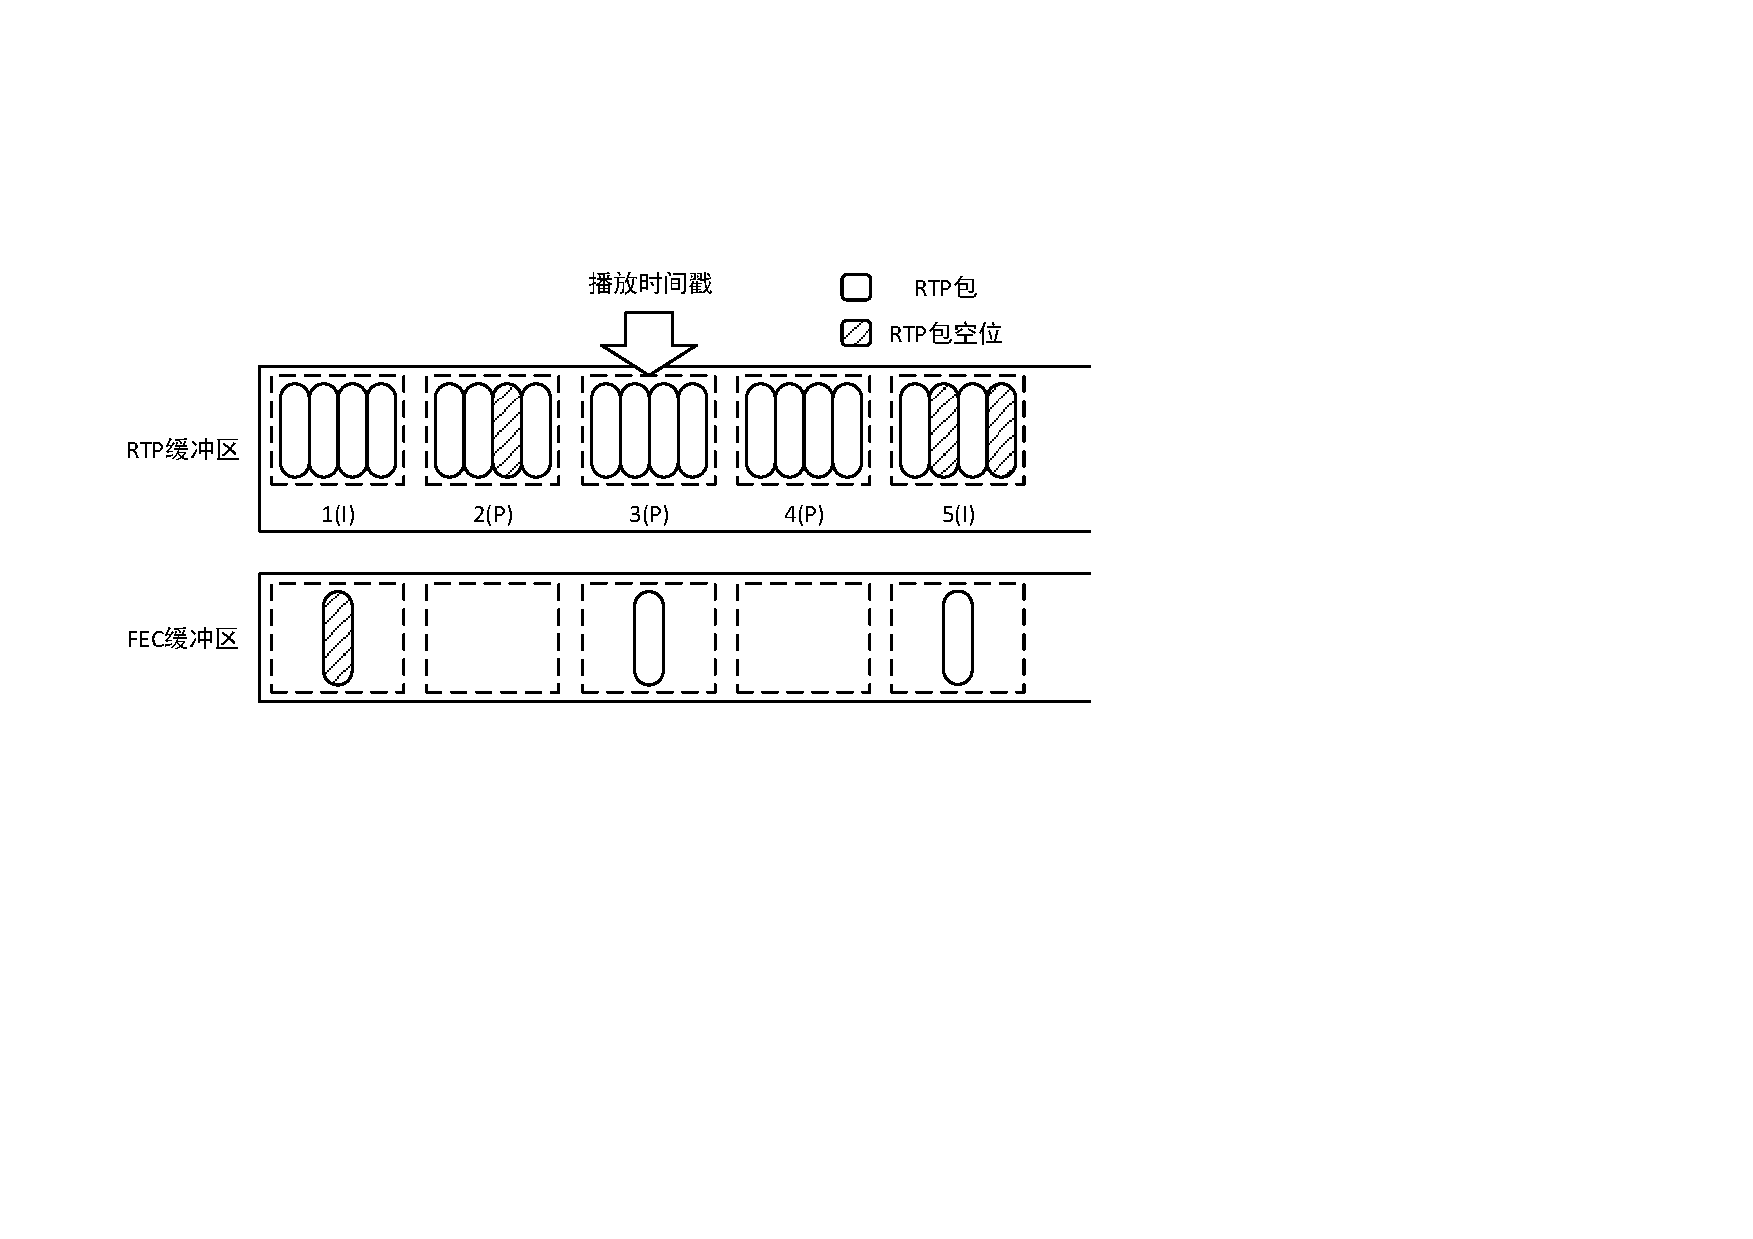
\includegraphics[width=0.9\textwidth]{fec_dec_buf.pdf}
      \caption{扩展窗口RS编码流程图}
      \label{fig:fec_dec_buf}
    \end{figure}

    在接收端,oRTP模块根据当前视频播放时间戳从RTP缓冲区中取出时间戳小于播放时间戳的所有RTP包(说明这些数据包所属视频帧已经到了播放的时间),输出到后续视频解码模块进行解码和播放。为了方便描述,我们在图 \ref{fig:fec_dec_buf}中给出了某一播放状态下的RTP缓冲区和FEC缓冲区状态,以及播放时间戳位置。如图所示,接收端的两个缓冲区中保存了当前待播放视频帧所在GOP 的所有已接收数据包(图中1/5为I帧,因此1-4属于同一GOP,待播放视频帧为3),及其之后的所有已接收数据包。当播放时间戳到达第3 帧并试图取RTP 包时,首先对1-3 帧所有数据包组成的编码块进行解码,此时第2 帧中丢失的RTP 包被恢复,RS解码过程结束。值得注意的是,如果不采用扩展窗口编码框架,那么图中第2 帧由于丢失数据包无法解码,根据GOP中视频帧之间的参考规则,后续的3、4 帧都将无法解码。而通过扩展窗口编码,第三帧的编码块同样包含了1/2帧的数据包,在解码时可以恢复他们丢失的数据包,尽管第2帧已经错过了播放时间,但通过缓冲区更新技术可以保证后续视频帧的解码。我们将在下一节介绍我们对缓冲区更新的实现。
    
    \subsubsection{``解码缓冲区更新''}
    在流式视频播放过程中,某些视频帧可能因为过大的延迟,在播放时刻之后才成功解码(如图 \ref{fig:fec_dec_buf} 中的第2帧)。由于这一视频帧已经无法再应用于播放,在很多视频通话应用中都直接将这些数据包丢弃而不再解码。然而这一视频帧除了用于播放之外,还可能被GOP中后续的视频帧引用,如果直接丢弃,则所有引用了该数据的视频帧都将无法解码,这可能造成GOP中所有后续视频帧的丢失。
    
    缓冲区更新就是针对以上问题的一种解决方法。当收到过期视频数据时,仍然对其进行解码,并将解码之后的数据更新到视频解码器的参考缓冲区中,使得后续视频帧能够成功解码。然而一方面缓冲区更新需要的操作逻辑比较复杂,对计算资源不足的智能设备压力较大,另一方面视频帧在播放时刻之后才能够成功解码这一现象发生几率较小,因此在一般视频通话应用中很少进行实现。   
    在我们的TVPhone中,由于添加了扩展窗口框架,GOP中已经播放的视频帧也有很大概率被解码,因此使用缓冲区更新技术能够大大提高视频帧的整体解码概率。为此,我们对前述``RTP接收缓冲区''的取数据过程进行了改进。
    
    在oRTP模块中,视频播放时间戳随着系统时间沿着RTP缓冲区不断向后移动,如图 \ref{fig:fec_dec_buf} 所示。每当经过一个视频帧,其所有数据包都直接被取出并传递给下一级的视频解码Filter,然而由于某些数据包可能缺失,在视频解码过程中失败,进而当前GOP中所有后续视频帧都无法成功解码。这一结果和发现某一视频帧不完整后直接在RTP缓冲区中丢弃这些数据包是相同的。与其如此,我们可以将这些数据包保留在RTP缓冲区中,直到GOP中最前面的视频帧数据完整,再一并取出解码,这样就等效实现了解码器的``缓冲区更新''。

    \begin{figure}[htbp]
      \centering
      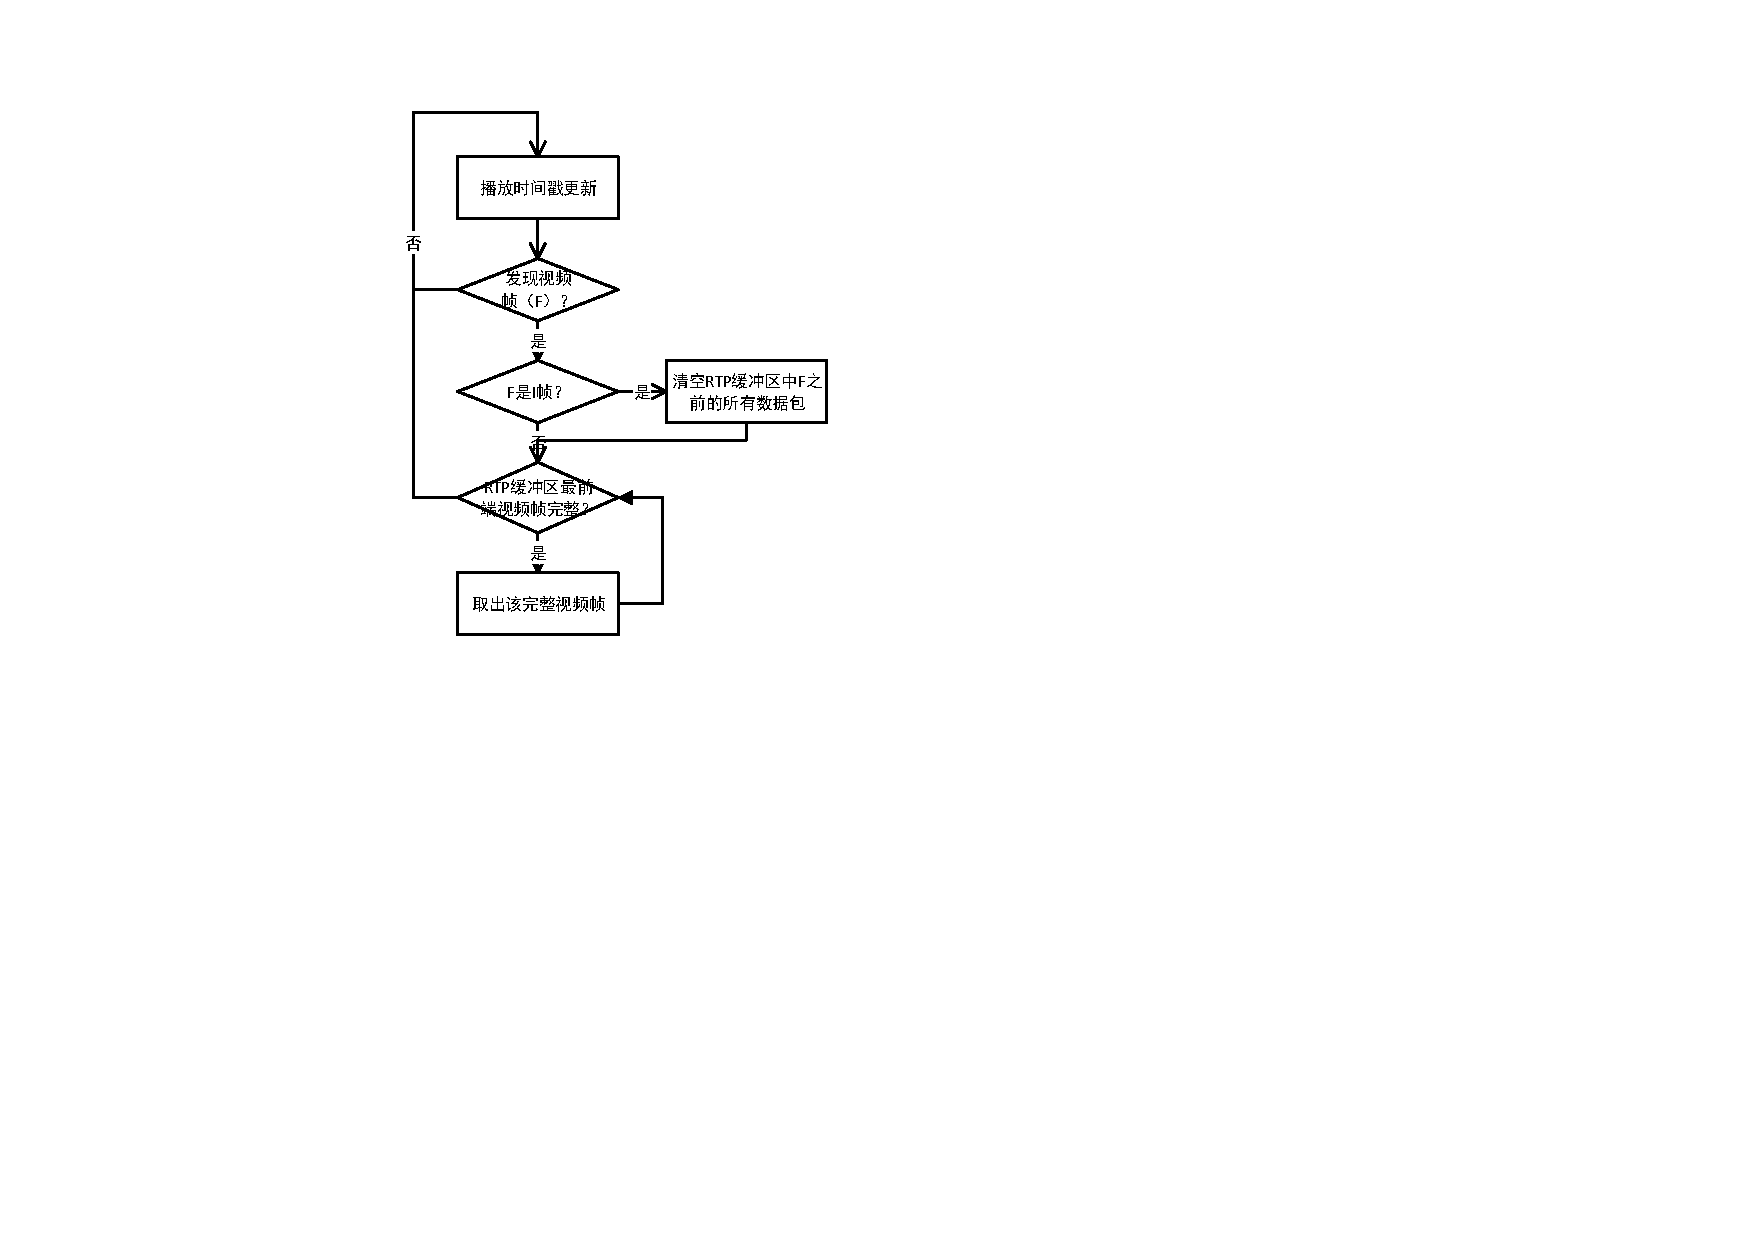
\includegraphics[width=0.5\textwidth]{fec_dec_buf_state.pdf}
      \caption{解码缓冲区更新}
      \label{fig:fec_dec_buf_state}
    \end{figure}
    
    上述操作逻辑如图 \ref{fig:fec_dec_buf_state}所示,当播放时间戳更新并发现了新的可供播放视频帧(记为F)时,首先检查F是否是I帧,也即新的GOP的起点。如果F是I帧,说明缓冲区中保存的之前视频帧已经不会再被参考,因此可以全部清空,并从F开始执行后续逻辑。在RTP缓冲区中,我们检查最前端的视频帧数据(可能是新的I帧,也可能是由于不完整而没有被取出的旧视频帧),如果是完整视频帧则将其取出进行视频解码和播放,并循环此过程直到取完所有播放时刻之前的完整视频帧。这一过程保证了送至视频解码器进行解码的所有视频帧,其参考帧都已经成功解码,其效果与更新解码缓冲区是相同的,而且节省了很多无效的视频解码操作。

    \subsubsection{冗余率和冗余分配优化}
    如果系统冗余率明显超出了纠正丢包所需的比例,会有大量冗余包得不到利用而造成网络带宽的浪费;而如果冗余率过低,又会造成大量丢包无法恢复,通话质量得不到保证。为了尽可能使冗余率适应网络需求,我们增加了一个简单的冗余率自适应功能。即如果网络丢包率连续三次高于 $5\%$ 则提高一档冗余率,如果网络丢包率连续三次低于 $1\%$ 则降低一档冗余率。经测试这一简单策略可以较好地实现网络变化时的冗余率自适应。

    针对第\ref{chap:fec}章中提出的冗余分配优化算法,我们需要根据当前网络的丢包率以及当前视频GOP中不同位置视频帧的特性计算合理的冗余分配方案。如果对于每个GOP都重新计算,将会严重增加客户端的计算负载,并且实时性也无法得到满足。因此我们每隔1分钟采样一次当前平均丢包率和GOP的视频帧特性,通过算法\ref{al:hc}计算最优冗余分配,并在下一次采样计算前的所有RS 编码中使用这一分配策略。


\subsection{面向电视盒子的界面优化}
基于上述对视频通话服务核心模块的增改,为了能够进一步体现高质量视频传输的效果并更好地服务于视频通话的需求,我们为TVPhone设计了一套面向电视盒子的交互界面。通过这一界面,用户可以使用遥控器进行操作,直接在电视屏幕上实现视频通话,获得更好的用户体验。本章简要介绍其中几个主要界面的设计和实现。

\begin{figure}[htbp]
  \centering
  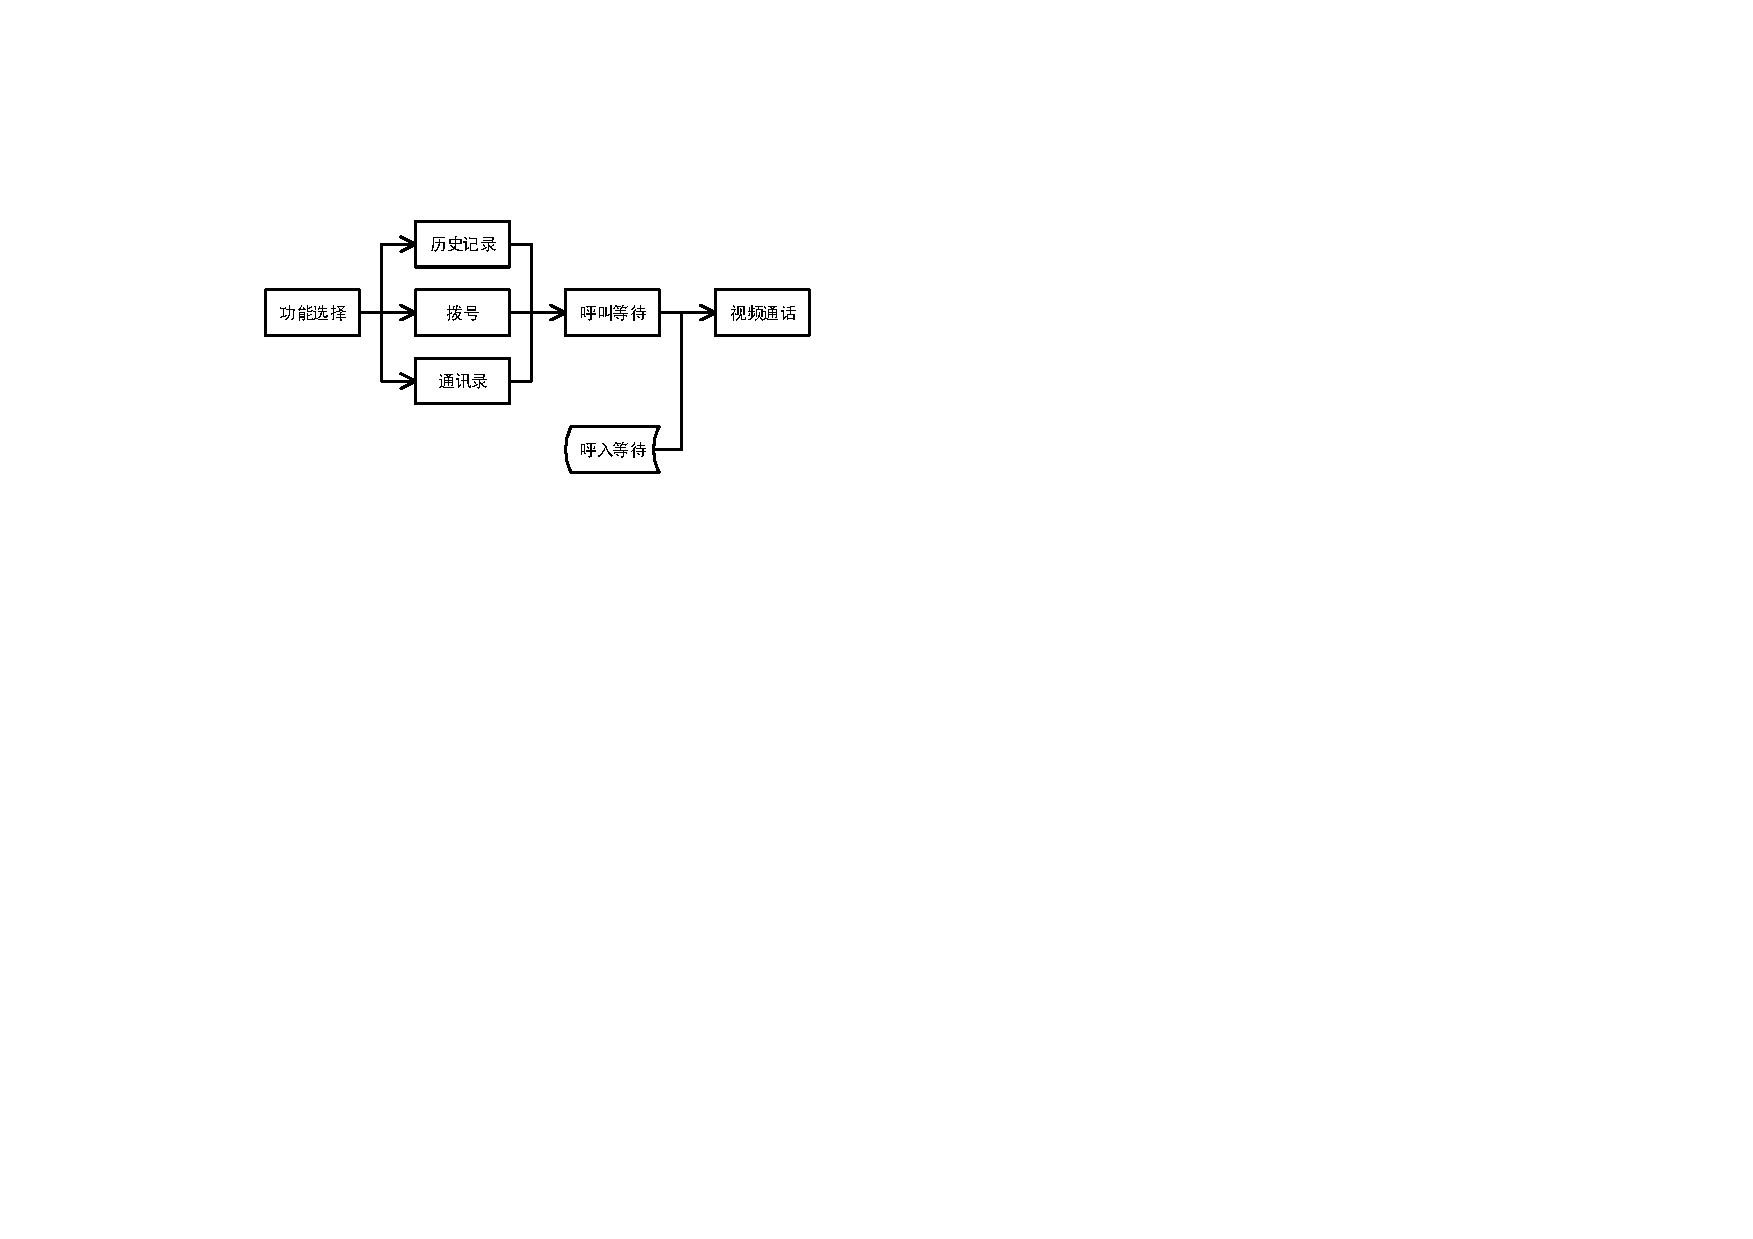
\includegraphics[width=0.7\textwidth]{ui_logic.pdf}
  \caption{页面跳转逻辑}
  \label{fig:ui_logic}
\end{figure}

本TVPhone视频通话系统的主要页面跳转逻辑如图\ref{fig:ui_logic}所示。应用启动后,首先出现功能选择界面\ref{fig:ui_main},用户可以选择的功能包括:历史记录界面查看最近的联系人并可以直接拨号;拨号界面\ref{fig:ui_call}通过输入对方的联系方式发起呼叫;通讯录界面\ref{fig:ui_contact}则记录了用户主动保存的联系人。在上述三个界面均可以方便地发起视频通话请求,进入呼叫等待界面等待对方接通。同时,软件在后台对呼入请求进行监听,发现呼入请求后转到呼入等待界面\ref{fig:ui_incall}。当通话双方均做好准备后,就可以打开视频通话界面开始高清视频通话。

\begin{figure}[htbp]
  \centering
  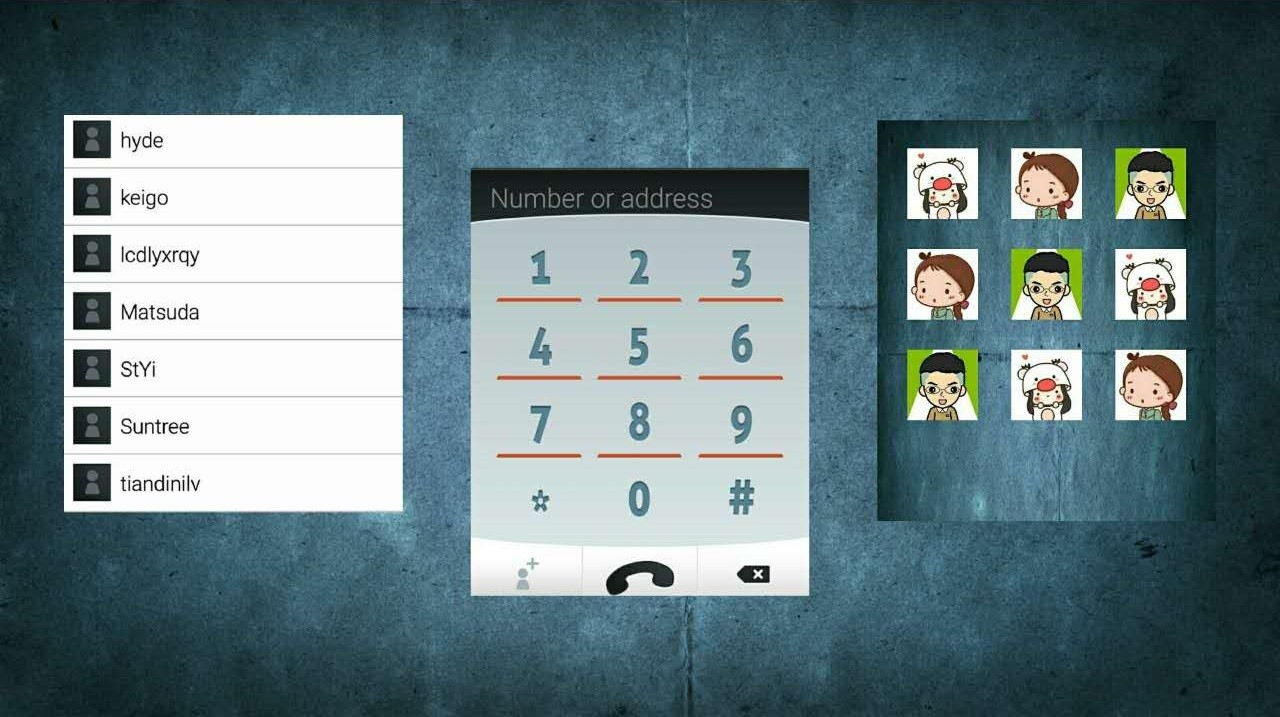
\includegraphics[width=0.6\textwidth]{ui_main.jpg}
  \caption{功能选择界面}
  \label{fig:ui_main}
\end{figure}

\begin{figure}[htbp]
  \centering
  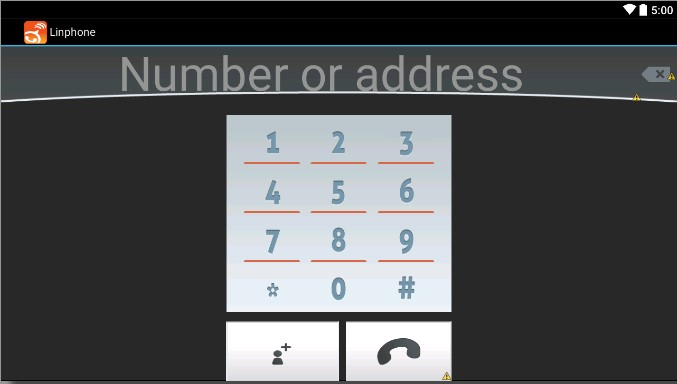
\includegraphics[width=0.6\textwidth]{ui_call.jpg}
  \caption{拨号界面}
  \label{fig:ui_call}
\end{figure}

\begin{figure}[htbp]
  \centering
  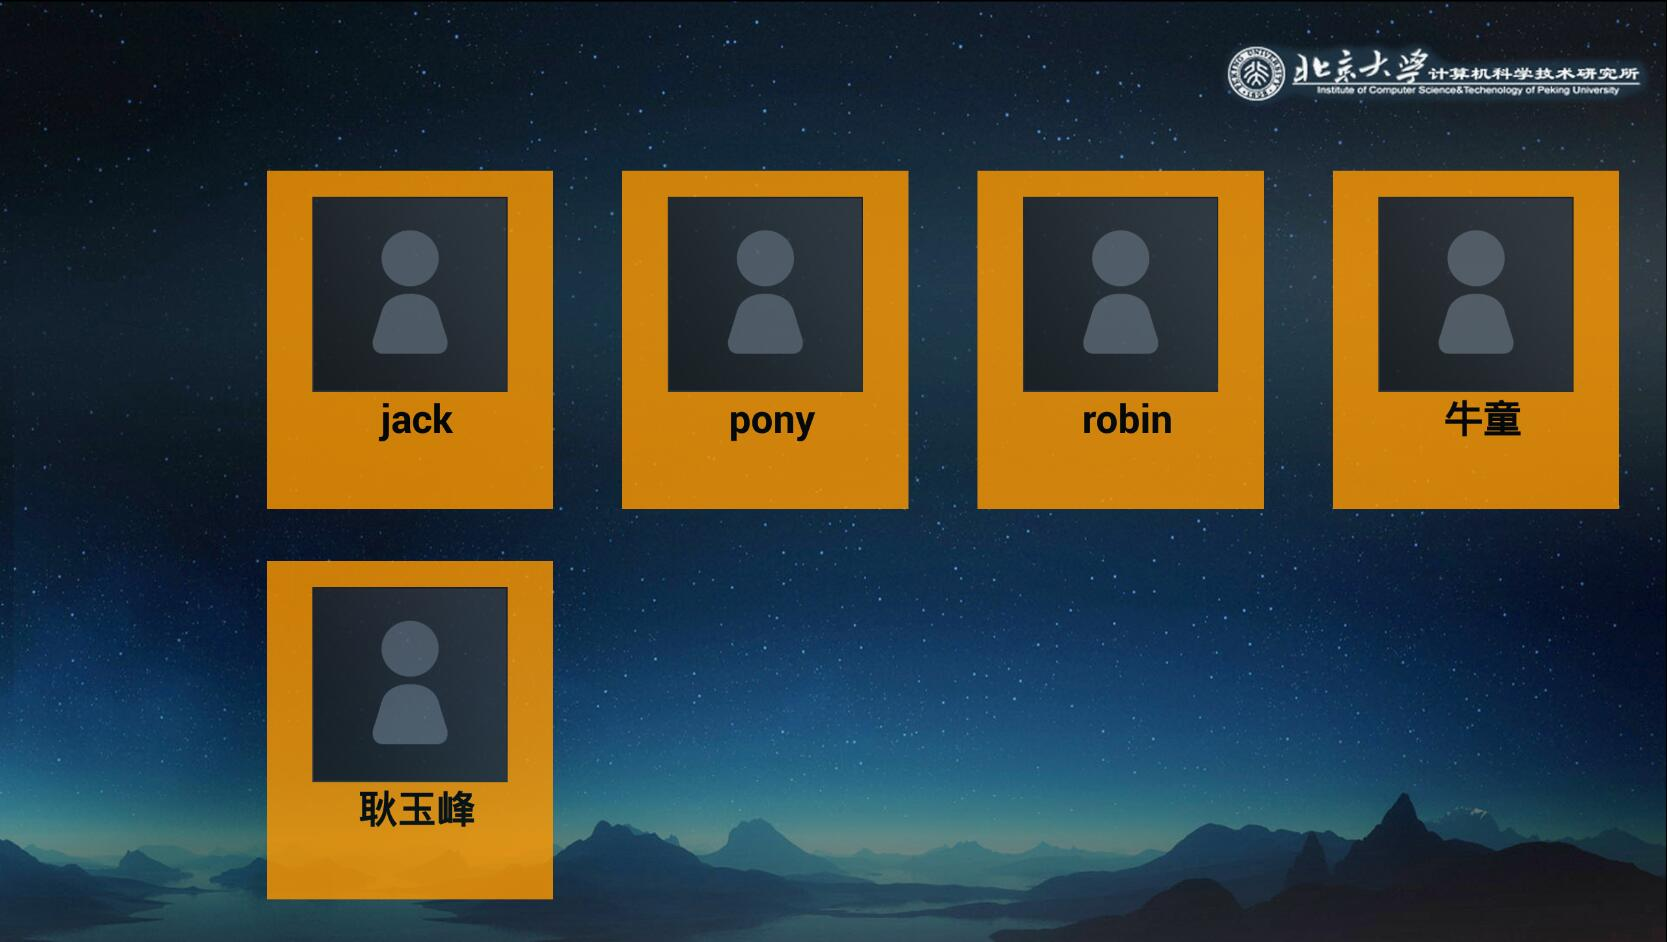
\includegraphics[width=0.6\textwidth]{ui_contact.jpg}
  \caption{通讯录界面}
  \label{fig:ui_contact}
\end{figure}

\begin{figure}[htbp]
  \centering
  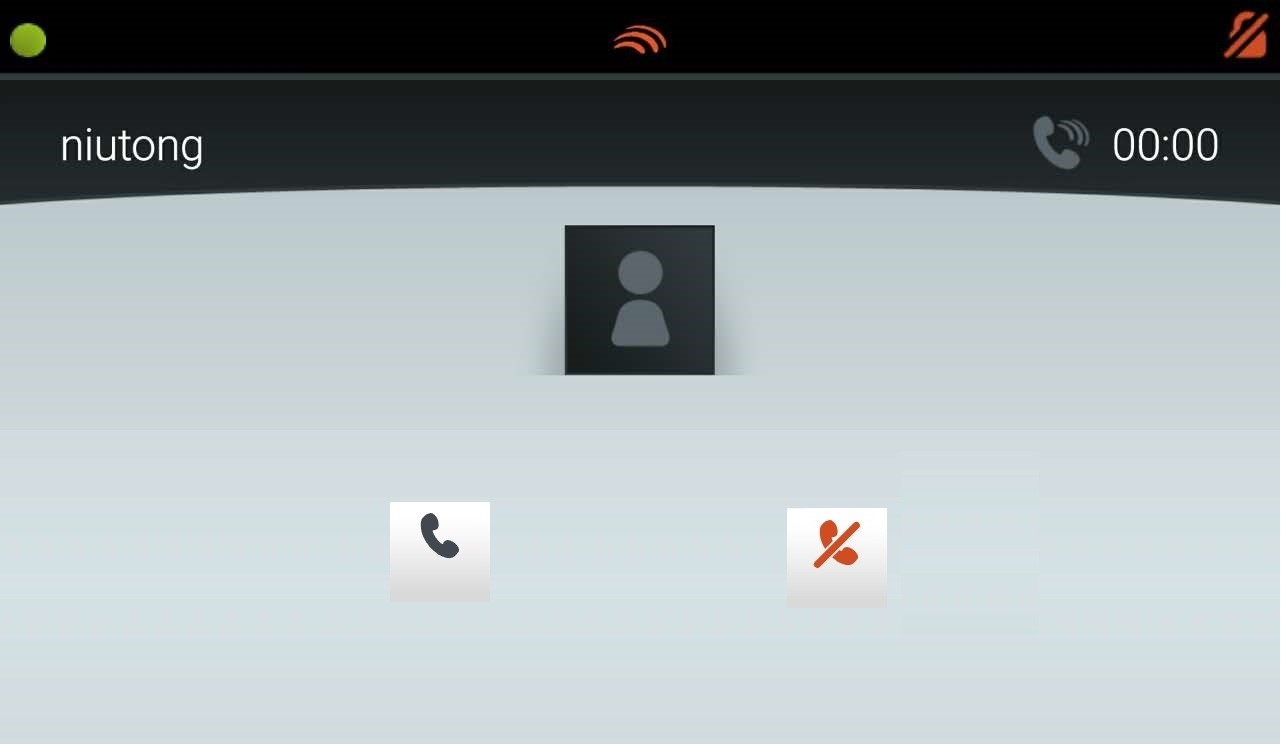
\includegraphics[width=0.6\textwidth]{ui_incall.jpg}
  \caption{呼叫等待界面}
  \label{fig:ui_incall}
\end{figure}

\section{实验验证}

TVPhone的目标是在无线网络环境下,提供面向手机和电视的高清视频通话服务。为了验证其服务效果,我们在手机和电视盒子上安装了TVPhone应用,并在真实无线网络环境下进行了测试。为了得到更全面的实验数据,我们还利用模拟器对不同网络状况进行了模拟,并对通话过程中的日志、视频文件进行记录和分析。

\subsection{实验设置}
\begin{figure}[htbp]
  \centering
  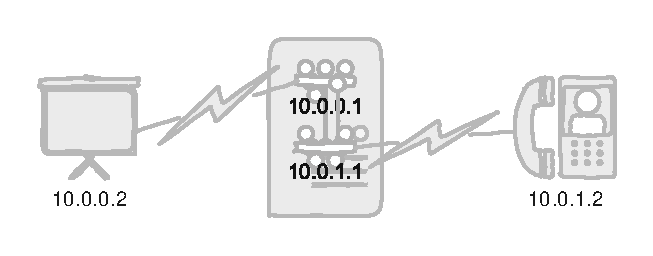
\includegraphics[width=0.6\textwidth]{exp_env.pdf}
  \caption{测试平台设置}
  \label{fig:exp_env}
\end{figure}

基本测试平台如图\ref{fig:exp_env}所示。为了对网络流量进行控制并检测网络利用情况,我们用一台具有双无线网卡的PC作为网络基站,建立两个处于不同网段(10.0.0.X 和10.0.1.X)的无线网络。视频通话终端是安装了TVPhone应用的手机和连接了电视盒子的电视,并分别连接两个无线网络。由于手机和电视处于不同网段,所有通信必须通过PC基站进行中转,我们就可以在PC基站上使用流量控制软件进行不同网络状况的模拟,如带宽限制、丢包、延迟等。


\subsection{结果分析}
%\textcolor{red}{目前本系统的核心算法和界面都还在最后准备中,最终结果分析会在系统完成后添加。预计时间为四月底。}

\begin{figure}[htbp]
  \begin{subfigure}[b]{0.5\textwidth}
    \centering
    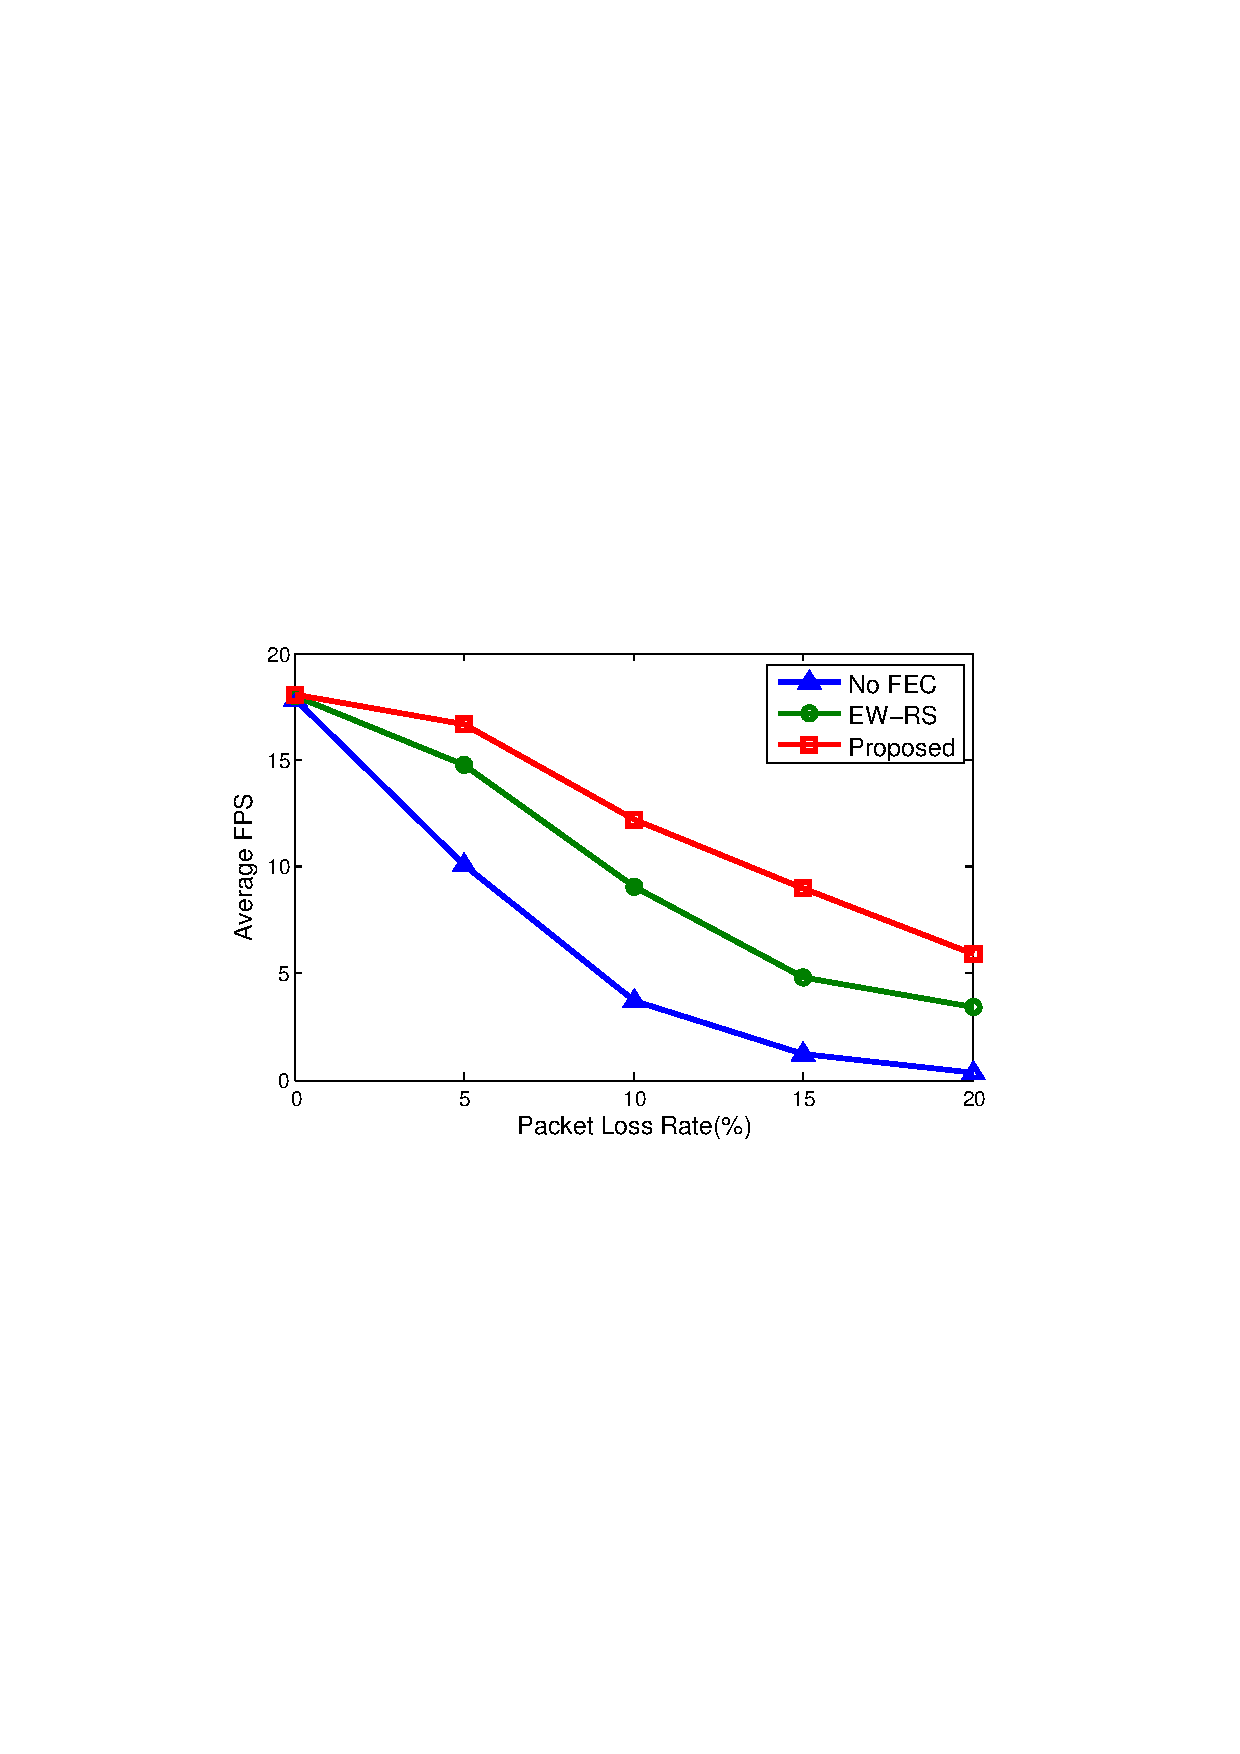
\includegraphics[scale=0.5]{tv_fps.pdf}
    \caption{帧率}
    \label{pic:tv_fps}
  \end{subfigure}
  \begin{subfigure}[b]{0.5\textwidth}
    \centering
    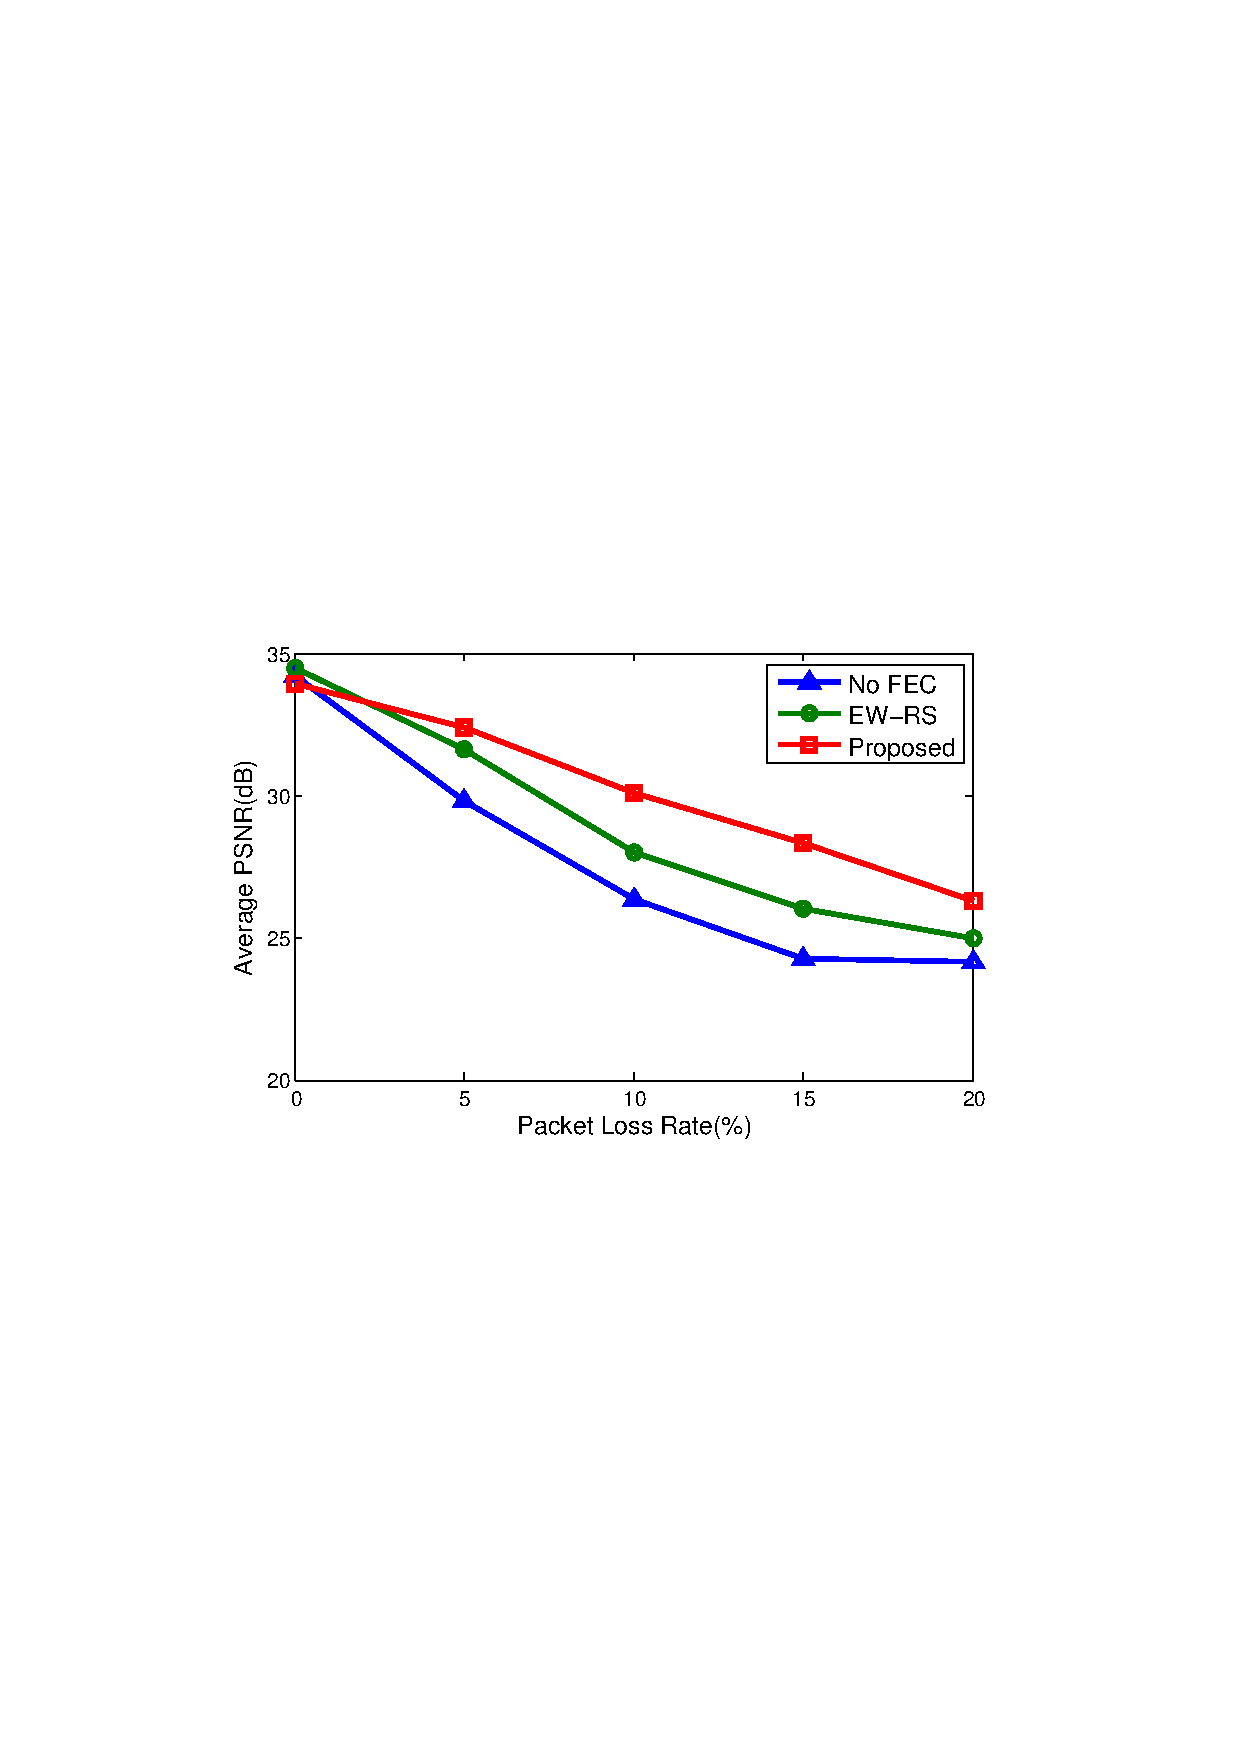
\includegraphics[scale=0.5]{tv_psnr.pdf}
    \caption{平均PSNR}
    \label{pic:tv_psnr}
  \end{subfigure}
  \caption{不同丢包率下系统表现}
  \label{fig:tv_loss}
\end{figure}

我们首先在设定相同FEC冗余率(约14\%)的条件下,通过模拟不同的网络丢包率测试原始Linphone和TVPhone对丢包的容错能力,图 \ref{fig:tv_loss}中``No FEC''表示不包括差错保护功能的Linphone实现,而``Normal FEC''和``Expanding Window''分别记录了TVPhone实现了普通的FEC算法和扩展窗口FEC算法的表现。在测试指标中,帧率(frame per second)体现了系统成功解码视频帧的能力,而平均PSNR 则更精确地分析了视频画面的效果。从图 \ref{fig:tv_loss} 可以看出,Linphone 由于没有FEC的保护,在丢包情况下大量视频帧无法解码,因而帧率随丢包率升高逐渐降低。同时由于帧率降低以及解码过程中由于丢包引入的画面失真,使得整体的PSNR 都下降明显。而TVPhone由于添加了差错保护模块,可以恢复部分丢包,因而帧率和PSNR表现都有很大提高。尤其是采用了扩展窗口编码框架后,丢包恢复能力进一步提高,即使在20\%丢包率的极端网络状况下,都能够保证最基本的视频通话效果。

\begin{figure}[htbp]
  \begin{subfigure}[b]{0.5\textwidth}
    \centering
    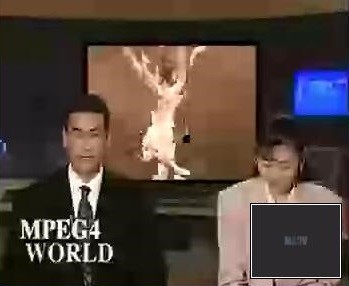
\includegraphics[scale=0.5]{exp_video1.jpg}
    \caption{Linphone}
    \label{pic:tv_fps}
  \end{subfigure}
  \begin{subfigure}[b]{0.5\textwidth}
    \centering
    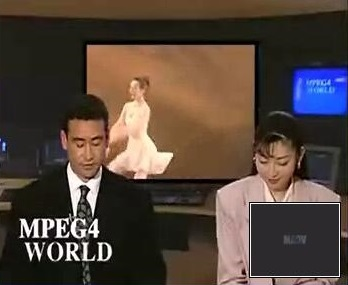
\includegraphics[scale=0.5]{exp_video2.jpg}
    \caption{TVPhone}
    \label{pic:tv_psnr}
  \end{subfigure}
  \caption{视频播放效果对比}
  \label{fig:exp_video}
\end{figure}

不同带宽条件下系统码率自适应算法的表现,我们已经在第 \ref{chap:rate}章进行过详细测试,这里不再赘述。

在真实网络环境测试中,我们在较差的Wifi信号条件下运行Linphone和TVPohne一段时间,两个系统在画面表现上具有较明显的差别。图 \ref{fig:exp_video} 截取了两个系统在模拟环境中运行的画面,从中可以看到,左侧的Linphone 通话画面画质较差,而且存在丢包造成的马赛克,与TVPhone 形成鲜明对比。

\section{本章小结}
在无线网络覆盖率越来越高,人们对视频通话需求日渐旺盛的背景下,我们利用算法上的优势实现了一个面向电视盒子的高清实时视频通话系统。为此,我们调研了一个开源视频通话软件,对其整体架构、各部分模块的具体实现、底层算法都进行了总结和梳理。以此为基础,我们将新的算法实现为独立模块植入原有系统中,解决了一系列代码实现和软件兼容问题,成功升级了该视频通话软件的内核,提高了其视频传输的质量。为了拓展高清视频通话的应用场景,我们还重新设计的该系统的用户界面,将其移植到大屏幕的电视盒子上,创造了一种新的高清视频通话体验。实验表明,我们的应用明显提升了视频通话的质量。

% !Mode:: "TeX:UTF-8"
% 文字编码:UTF-8
\chapter{延迟优化的实时视频码率自适应算法}
\label{chap:rate}

\section{引言}
随着移动智能设备和移动网络的普及,基于无线网络的实时视频通信的应用也越来越广泛。然而,在无线网络上进行实时视频传输还面临着带宽、延迟波动,物理链路丢包等挑战。为了避免网络拥塞引起的路由器主动丢包、延迟波动和带宽浪费,传统网络应用都需要采用TCP协议等对数据流进行拥塞控制。而在实时视频传输中,我们也必须要对视频流进行码率自适应。

视频传输码率自适应算法一直是一个活跃在学术界和工业界的热门问题,并且在TCP等传统拥塞控制算法的基础上发展出了不同的实现思路和方法。在第 \ref{chap:related}章,我们介绍了在网络传输尤其是实时视频传输过程中使用的主要码率自适应算法。本文从输入信号以及码率控制方式两个角度对主流实时视频码率自适应方法进行了分类。

首先,视频码率自适应算法作为一种网络拥塞控制算法,针对网络的负载状况反馈进行针对性的码率调整,必然要以网络真实参数作为输入信号,这些信号包括:
\begin{itemize}
    \item \textbf{丢包}:尽管无线网络由于信道质量差,发生丢包的概率较大,但丢包最主要的原因还是网络发生拥塞后在路由器上进行的主动丢包。因此,丢包也成为传统拥塞控制协议探测网络丢包的最主要手段。尽管如此,丢包信号应用在面向无线网络的数据传输中却并不合适。这是因为无线网络由于物理信道质量差,在没有网络拥塞的情况下丢包率也比较高,这会使拥塞控制算法低估网络带宽,造成带宽浪费。而且一旦网络拥塞引起了丢包,就说明网络已经发生了严重拥堵,这时延迟和抖动都非常严重,对实时视频通话效果的影响将需要很长时间恢复。
    \item \textbf{传输延迟}:数据从准备发送到成功接收之间的端到端延迟,通常用往返时延(Round Trip Time, RTT)衡量,主要包括:发送端数据处理、各中间路由器转发前的排队缓存、数据推送到传输介质以及数据在传输介质中传播四种不同延迟组成。其中唯一随网络状况有较大变化的就是数据包在中间路由器的排队缓存时间(我们称之为排队延迟),网络负载越大,缓存时间越长,排队延迟越大。因此,网络延迟也成为使用越来越多的拥塞控制信号。相对丢包而言,以网络延迟作为拥塞信号,可以根据延迟的增减情况判断网络状况的渐进变化,提前对视频码率进行调整以避免出现网络延迟,因而可以很好地保证视频数据传输的平稳高效。
    \item \textbf{抖动}:如果网络带宽、负载波动较大,就会使延迟出现较大波动,这一抖动尤其对延迟敏感的实时传输影响较大。因此延迟的相对抖动也成为视频码率自适应中需要参考的一种重要网络信号。
\end{itemize}
尽管在第 \ref{chap:related}章中提到的ECN标记也可以作为网络拥塞信号,但这类依赖于网络硬件参与的反馈信号需要对现有设备进行大规模改造,在通用算法中一般不予考虑。因此以上三条基本涵盖了主流拥塞控制算法所使用的反馈信号,当然在实际算法中可以综合利用其中的多种信号进行码率控制。

另外,从码率控制方式的角度进行总结,我们将主流拥塞控制算法分为以下三类:
\begin{itemize}
    \item 基于拥塞信号探测的控制。这类拥塞控制算法通过不断增加码率,直到网络达到某一可检测的阈值(例如丢包率达到某一阈值$P_{th}$\cite{wu2000end})来对网络带宽进行探测。常用的探测过程包括AIMD和MIMD 两种。这一控制方法通过控制网络保持在拥塞阈值之下来避免拥塞,但这一方法也导致网络延迟一直保持在较高水平。另外,当网络达到阈值时,为了避免即将发生的拥塞,必须大幅度降低发送速率(乘性减),因此发送码率波动较大,带宽利用率也相应较低。
    \item 基于网络模型的控制。与上述方法隐式估计网络带宽不同,基于模型的拥塞控制对网络建立公式描述,并计算相应的发送速率,以此显式地估计网络带宽。一种典型的应用是TFRC协议。一些基于控制论的方案也需要先建立网络控制模型,描述发送速率与网络参数之间的关系,从而建立闭环控制框图。
    \item 基于状态机的控制。随着视频通话应用不断涌现,在实际工程中一种基于状态机的算法应用越来越广泛。这一控制方法通过状态机对网络的不同状态进行描述,并通过一定条件触发状态间的转移。对于不同的网络状态,则采取不同的码率调整策略。通过对状态机的状态、跳转、行为等进行较细致的定义,可以给出比较复杂的控制系统,拟合不同的网络情境并充分结合应用测试中的经验。但这也成为该控制方法的一个缺点:模型和参数设定过分依赖工程经验,没有系统的优化方法,缺少理论支持。
\end{itemize}

我们的电视盒子视频通话系统主要应用场景是网络状况波动较大、丢包率较高的无线网络,在此背景下,大部分现有算法都不能对带宽进行有效利用。如基于丢包的算法存在带宽低估、延迟过大的问题;大部分算法都不能提供延迟波动范围的保证等。针对现有码率自适应算法的不足,我们希望设计一种针对无线网络实时视频传输的码率自适应算法,综合考虑无线网络高丢包的特点以及实时视频低延迟、稳定带宽的需求。这一算法的实现目标包括:
\begin{itemize}
    \item 在高丢包网络中准确估计真实带宽
    \item 稳定的低传输延迟
    \item 在带宽波动时反应灵敏、调整过程平滑
    \item 多流竞争公平性
\end{itemize}

为了实现上述目标,我们以控制论为基础,结合对网络排队延迟的建模,设计了一种延迟可控的视频码率自适应算法。首先,通过对带宽限制下的多流竞争系统建模和推导,我们引入了一个流式排队模型来对网络数据流的效率、稳定性、公平性进行分析。在这一流式排队模型中,通过控制排队延迟在一定范围内波动就可以完成网络拥塞控制。一种直观的理解是:当排队延迟超出预定值或增长过快时,通过及时降低视频码率来避免网络拥塞;当排队延迟低于预定值或下降过快时,通过提高视频码率来充分利用过剩的网络带宽。
我们将这一控制策略建模成非线性闭环控制模型,并对其进行线性化以利于进一步分析优化。最后,为了进一步提高系统性能,我们引入PID控制器,通过分析系统的稳定性和响应时间,对系统参数进行优化,从而为视频选择更加合适的码率。

%\section{带宽限制下的多流竞争分析}
%\label{section:shadow_price}
%
%在网络传输过程中,我们希望在有限的网络带宽限制下,为所有共享这一网络的用户提供更高的整体效用,这一问题可以用如下带约束的优化问题描述:
%\begin{equation}
%\label{eq:system_problem}
%\begin{aligned}
%& \max_{x_i}
%& & \sum_{i=0}^N{U(x_i)} \\
%& \text{s.t.}
%& & \sum_{i=0}^N{x_i} \leq C \\
%&&& x_i \geq 0, \; i = 1, \ldots, N.
%\end{aligned}
%\end{equation}
%$x_r$表示第$r$条数据流的发送速率,$U(x_r)$表示第$r$条流在发送速率$x_r$条件下获得的效用。所有数据流的发送速率$x_r$之和必须小于网络带宽$C$ 且不能为负数。
%在最优化问题中,拉格朗日乘数法是一种寻找多元函数在变量受到一个或多个条件的约束时的极值的方法。此问题中我们引入拉格朗日乘子$\lambda$并得到如下拉格朗日函数:
%\begin{equation}
%\label{eq:lagrangian}
%  \max L(x_i, \lambda) = \sum_{i=0}^N{U(x_i)} + \lambda (C-\sum_{i=0}^N{x_i})
%\end{equation}
%其中拉格朗日乘子$\lambda$也被称为影子价格。求解这一无约束形式的一阶条件包含如下约束:
%\begin{equation}
%\label{eq:FOC}
%  \frac{\partial L(x_i, \lambda)}{\partial x_i} = U'(x_r) - \lambda = 0
%\end{equation}
%
%在式 \ref{eq:FOC}中,由于我们还未给出$U(x)$的定义,因而暂时无法求解式 \ref{eq:system_problem}中的优化问题。根据常识可知,$U(x)$满足边际效用递减原理(即码率越大,增加单位码率对效用的提升越小),记为$U'(x) < 0$。 因此,尽管模型参数还未确定,我们可以使用渐进法逐步逼近$x$ 的准确值。渐进法形式如下:
%\begin{equation}
%\label{eq:approach}
%  x_i' = k ( U'(x_i) - \lambda)
%\end{equation}


\section{流式排队模型}
在以分组交换为基础的互联网数据传输中,用户数据被分割封装为包含了地址和管理信息的分组,分组通过最佳路径路由到目标,中间经过了路由器或交换机的层层转发。
以太网路由器的工作原理是存储转发,即先将输入端口到来的数据包缓存起来,按顺序对它们进行处理,因此也引入了较大的数据包处理延迟。
如果短时间内进入网络的数据包数量超出了网络的处理能力,就会在中间路由器堆积,形成网络拥塞。并进一步引起排队延迟增大,甚至路由器缓冲区溢出后发生大量丢包。

\begin{figure}[htbp]
  \centering
  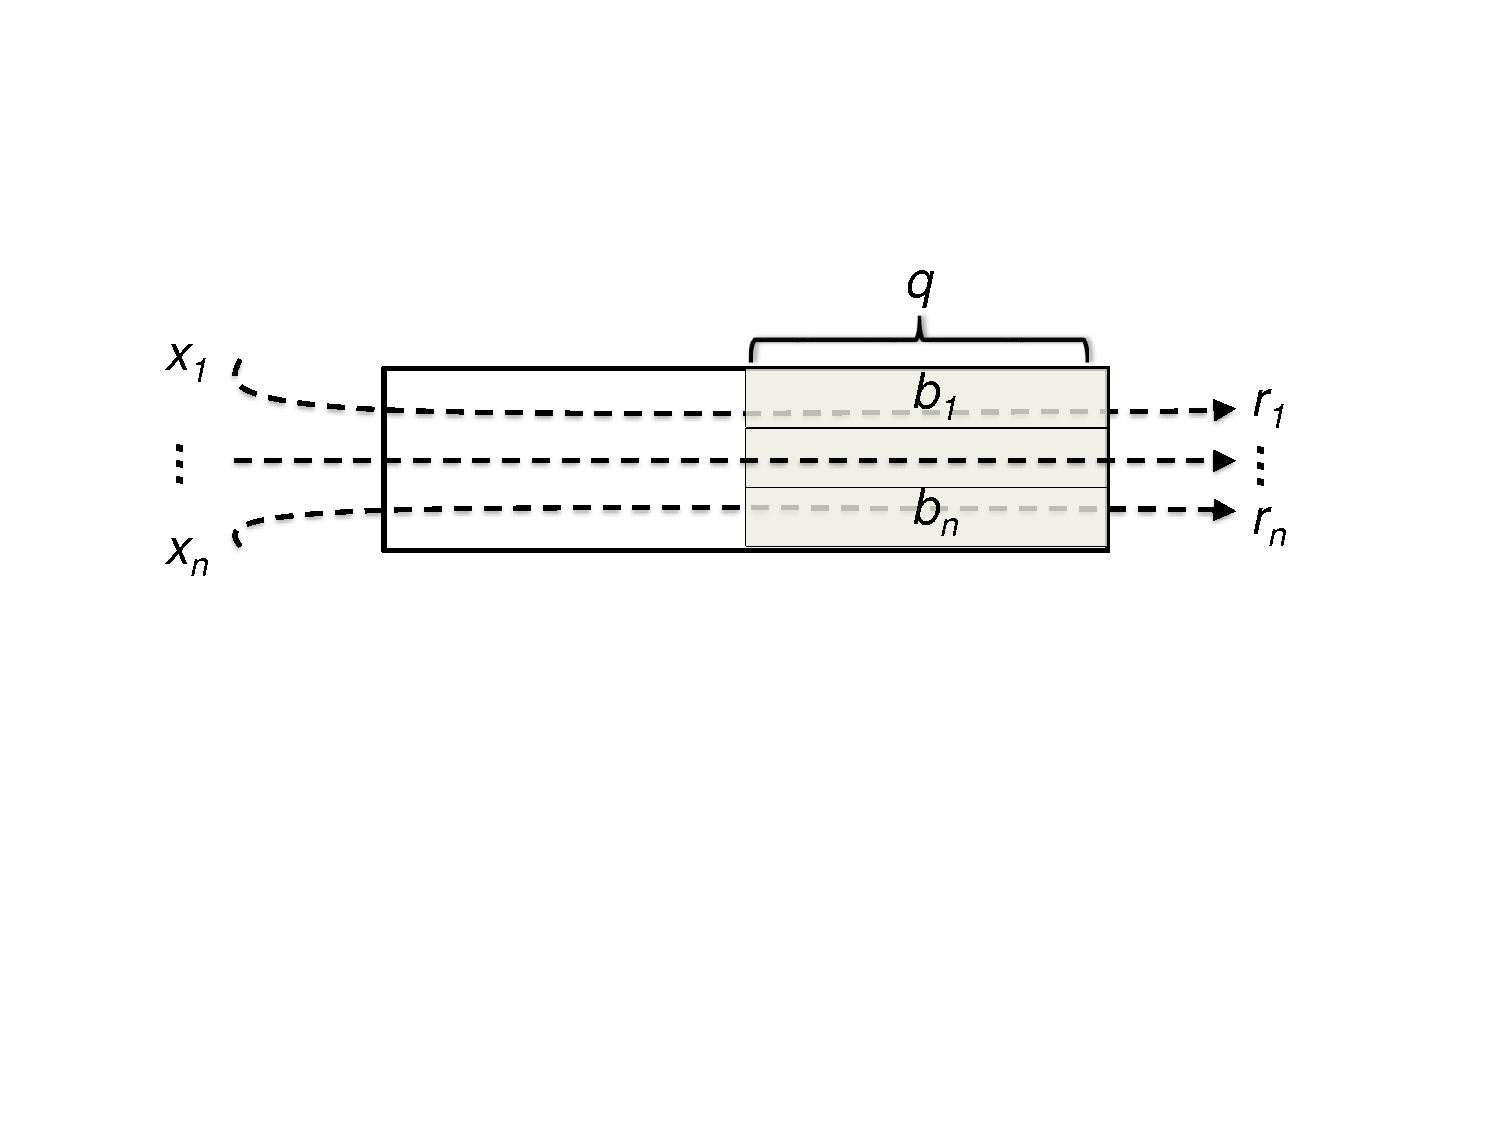
\includegraphics[width=0.5\textwidth]{buffer.pdf}
  \caption{流式排队模型}
  \label{fig:buffer}
\end{figure}

为了描述这一数据传输过程,我们通过图\ref{fig:buffer}所示的流式排队模型来对网络链路进行建模。我们将一条数据链路上的所有中间路由器简化为一个进行``存储-转发''的缓冲区,$N$ 个数据流在同一链路上进行数据传输,所有数据包都需要经过这一缓冲区才能达到目的地,因此形成对带宽资源的竞争。
假设第$i$ 条流占据的缓冲区数据量为$b_i$,其数据发送速率为$x_i$,从排队论的角度,整个缓冲区队列的入队速率为$\sum_{i=1}^N{x_i}$,其排空速率则始终等于网络带宽$C$。对于这一缓冲区的角度,有:
\begin{equation}
\label{eq:buffer}
  b'(t) = \sum_{i=1}^N{x_i(t)} - C
\end{equation}
其中 $b'(t)=db/dt$ 代表缓冲区大小随时间 $t$ 的变化速率。

图中 $q$ 表示前文提到的排队延迟,即数据包通过该缓冲区需要的时间。其含义为一个数据包进入缓冲区后,需要等待所有之前的数据包全部处理完毕才能通过缓冲区,这一过程即为``排队''。根据排队论,有:
\begin{equation}
\label{eq:delay}
    q(t) = \frac{b(t)}{C}
\end{equation}

考虑到单个网络流没有链路上的其他数据流的信息,为了达到系统的稳定公平,我们结合已有研究引入了基于影子价格 \cite{kelly1997charging}的码率控制模型。
首先根据视频数据的率失真曲线\cite{berger1971rate}赋予每条数据流权重 $\omega$,该权重值使每条视频数据流基于率失真公平性竞争带宽。如高清视频相对于普通视频具有更高的编码码率,因此可以设定较大的$\omega$以获得足够的带宽。
数据流对于获取的带宽需要付出价格为 $p(t)$ 的拥塞代价。利用失真权重和影子价格的码率控制模型可以描述为
\begin{equation}
\label{eq:rate}
    x_i'(t) = \omega_i - x_i(t)p_i(t)
\end{equation}
其中 $x_i'(t)=dx_i/dt$ 代表码率随时间的变化速率。

所有视频流根据式\ref{eq:rate}调整视频码率。当网络接近拥塞时,码率较高的视频流由于付出更大的拥塞代价,码率下降更快。经过一段时间的动态调整,所有视频流都稳定在失真公平的码率附近。与直接参考传输延迟的值进行码率控制的 FAST TCP\cite{wei2006fast} 等协议不同的是,我们以拥塞代价$p(t)$作为中间值,解耦了码率控制和延迟之间的直接关系,从而使调节过程更加灵活,避免了调节过程中的延迟积累、波动等问题。


\section{闭环码率控制模型及其线性化}
在实际应用场景中,不同用户进行视频通话的质量各不相同,而他们之间带宽竞争的公平性在不同衡量标准(如使用带宽分配情况、视频清晰度、用户满意程度)下具有不同的结果,这本身就是一个值得研究的问题。在本文中,为了简化分析过程,我们假设所有用户是同质的,即他们具有同样的视频权重 $\omega$ ,因而系统稳定状态下,每个人获得的发送速率$x$也应该相等。这样式\ref{eq:buffer}-\ref{eq:rate}可以简化为
\begin{equation}
\label{eq:rate_model}
\left\{\begin{array}{l}
    x' = \omega - xp \\
    b' = Nx - C\\
    q = \frac{b}{C} + t_p
\end{array} \right.
\end{equation}

从控制论的角度看,上述系统是一个分析难度很大的非线性系统。为了简化分析,我们在其稳定点取差分,从而将其等效转化为线性系统。记其稳定点的影子价格为$p_0$,对应发送速率为$x_0$,且稳定点满足$x'=0$,则:
\begin{equation}
x'=0 \Longrightarrow \left\{\begin{array}{l}
    \omega = x_0 p_0\\
    x_0 = \frac{C}{N}
\end{array} \right.
\end{equation}

\begin{figure}[htbp]
  \centering
  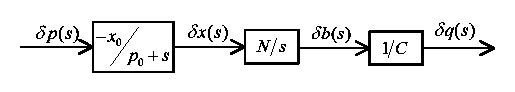
\includegraphics[width=0.7\textwidth]{block2.eps}
  \caption{复数域控制系统框图}
  \label{fig:block2}
\end{figure}

对各参数进行差分操作$\delta p(t)=p_0 - p(t)$, $\delta x(t) = x_0 - x(t)$ 和 $\delta q(t) =q_0 - q(t)$,得到线性化之后的码率控制系统如下:
\begin{equation}
\label{eq:linear}
\left\{\begin{array}{l}
    \delta b'(t) = \sum_{i=1}^{N}{\delta x(t)}  \\
    \delta q(t)  = \frac{\delta b(t)}{C} \\
    \delta x'(t) = -p_0\delta x(t) - x_0 \delta p(t)
\end{array} \right.
\end{equation}
根据控制论对式 \ref{eq:linear} 进行拉普拉斯变换,得到该控制系统在复数域的控制框图如图\ref{fig:block2}所示。

\begin{figure}[htbp]
  \centering
  \includegraphics[width=0.8\textwidth]{block3.eps}
  \caption{闭环控制系统框图}
  \label{fig:block3}
\end{figure}

显然上述控制模型还没有形成闭环控制逻辑,其中缺失的关键环节就是系统输出的排队延迟与系统输入的拥塞代价之间的关系。
前文已经提到,拥塞代价是排队延迟与视频码率这一对控制变量之间插入的中间变量,在该控制模型中,我们的主要目标是以排队延迟作为系统反馈,来控制数据流的影子价格$p$,进而根据式 \ref{eq:rate}决定视频码率。根据图\ref{fig:block2}及控制论知识,我们在控制框图中添加一个以$\delta q(s)$为输入,$\delta p(s)$为输出的控制器$G_c(s)$
\begin{equation}
\delta p(s) = G_c(s)\delta q(t)
\label{equ_x_dif}
\end{equation}
完成这一控制过程,从而形成一个如图 \ref{fig:block3}所示的闭环反馈控制系统。

\section{PID控制器设计}
PID(比例-积分-微分)控制器是一种反馈回路部件,经常应用在工业控制系统中。这个控制器把收集到的数据和一个参考值进行比较,然后把这个差别用于计算新的输入值,这个新的输入值的目的是可以让系统的数据达到或者保持在参考值。PID控制器可以根据历史数据和差别的出现率来调整输入值,使系统更加准确而稳定。

PID控制器的比例单元P、积分单元I和微分单元D分别对应目前误差、过去累计误差及未来误差。在本文中,综合考虑控制效果和系统求解复杂度,我们选择比例控制器作为$G_c(s)$的实现,即
\begin{equation}\label{eq:gcs}
    G_c(s) = K_P
\end{equation}

不同的$K_P$取值决定了整个控制系统能否稳定,以及系统的响应时间等重要性能。为了对此进行分析,我们结合图\ref{fig:block3}和式\ref{eq:gcs}推导出该闭环控制系统的转移方程如下:
\begin{equation}\label{eq:transfer}
    H(s) = \frac{K_P}{s^2 + s p_0 + K_P} = \frac{\omega^2}{s^2 + 2 \zeta \omega s + \omega^2}
\end{equation}
其中$\zeta$代表系统的阻尼比,描述系统在受到扰动后振荡及衰减的情形。$\omega$代表系统的固有频率,即系统受到扰动后在无阻尼条件下的振荡频率。由上式可知$2 \zeta \omega = p_0$ 且$\omega^2 = K_P$,从而得到$\zeta = \frac{p_0}{2\sqrt{K_P}}$。为了得到良好的系统响应,我们选择已被证明具有较好系统表现的阻尼比$\zeta = \frac{\sqrt{2}}{2}$\cite{franklin2006feedback},则有
\begin{equation}\label{eq:k}
    K_P = \frac{p_0^2}{2}
\end{equation}
在以上取值条件下,系统的$5\%$稳定时间$T_s = \frac{6}{p_0}$。即当系统发生随机扰动后,在不超过$\frac{p_0^2}{2}$的时间内,系统可以调整到与目标码率差值不超过$5\%$的码率范围内,因此通过恰当的参数取值,可以保证系统的响应速度。


\section{实现细节说明}
为了方便地测试本文提出的码率自适应算法的效果,以及与现有算法的性能对比,我们基于前述开源软件Linphone的底层视频传输模块——Mediastreamer2,搭建了算法测试平台。基于视频码率自适应算法,我们实现了一个包含网络信息采集和发送、最优码率计算等功能的码率自适应模块。除此之外的大部分功能(如视频采集、码率可变编解码等)都沿用了已有实现。本节中,我们简要介绍一些系统实现中的重要细节。

    \subsection{排队延迟的计算}\label{chap:qd_calc}
    在数据传输过程中,传输延迟定义为数据包从发送端开始发送到接收端成功接收之间的时间间隔。其直观测量方式就是对数据包发送和接收时刻分别获取当前时间并作差,这一差值定义为单向延迟(One Way Delay, OWD)。然而,由于发送和接收两个客户端的时间设置很难保证完全同步,在单向延迟的计算中一个无法排除的误差就是时钟偏差。因此,在实际网络应用中,衡量网络延迟使用的一般是往返时延(Round-Trip Time, RTT)这一变量,表示从发送端发送数据开始,到发送端收到来自接收端的确认(接收端收到数据后便立即发送确认),总共经历的时延。

    在视频通话过程中,视频流是双向同时进行的,但由于网络环境的多样性,不同方向上的网络状况可能存在很大区别。如果采用RTT作为延迟信号,我们只能获得上下行两个方向上的延迟之和,因而无法针对单向链路进行针对性的码率调整。在本研究中,利用即将给出的排队延迟的特性,我们可以消除单向延迟存在时钟偏差的问题,因而可以采用单向延迟进行更加精确的码率调整。

    由单向延迟的定义我们知道
    \begin{equation}\label{eq:owd}
        OWD = D_q + D_t
    \end{equation}
    其中$D_q$为排队延迟,$D_t$为除排队延迟以外的其他延迟,这部分延迟主要与网络物理环境有关,因此连接建立后变动很小。因此,我们可以通过如下方式计算排队延迟
    \begin{equation}\label{eq:qd}
        D_q = OWD - OWD_{min}
    \end{equation}
    其中$OWD_{min}$是传输过程中单向延迟的最小值,在每次计算单向延迟时更新。考虑到当网络负载达到最小时,数据包在所有路由器上都直接被处理,则其延迟中将不包含排队延迟,我们认为这一最小值可以很好地估计网络的固定时延。同时在对单向延迟作差的过程中,我们已经消除了时钟偏差这一误差。

    \subsection{影子价格的更新}
    由式 \ref{eq:gcs}定义的比例控制器,有
    \begin{equation}\label{eq:kpt}
        \delta p = K_P \delta q
    \end{equation}
    在系统实现角度,由于不同的视频流特性、网络状况等,不同系统具有不同的系统取值,我们不可能提前知道任一系统达到稳态时对应的影子价格$p_0$。然而注意到上式中排队延迟和影子价格都是差分形式,将其展开后有:
    \begin{equation}
        p(t) = p(t-1) + K_p(q(t) - q(t-1))
    \end{equation}
    通过这一变形,我们可以在系统运行过程中逐步逼近正确的影子价格。同时根据式\ref{eq:k}动态更新相应的$K_P$值。

    \subsection{视频码率控制}
    式 \ref{eq:rate}给出了时间连续的系统中码率的变化率公式,然而在实际系统中,调整间隔不可能无限小。我们去单词码率调整的时间间隔为$\Delta{T}$,则在此离散的码率调整方式下码率计算公式为
    \begin{equation}
        x(t) = x(t-1) + x'(t) \Delta{T}
    \end{equation}

    我们在每个时间片起始时更新视频码率。系统启动时,视频码率被设定为编码器允许的最小值,如64Kbps。


\section{实验验证}
本小节中,我们基于实验平台对我们的码率自适应算法进行了测试,并与几种主流拥塞控制算法进行了对比。

    \subsection{实验设置}

    \begin{figure}[htbp]
      \centering
      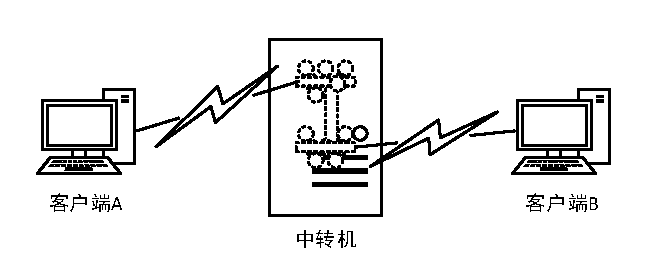
\includegraphics[width=0.6\textwidth]{rate_exp_arch.pdf}
      \caption{测试平台设置}
      \label{fig:rate_exp_arch}
    \end{figure}

    如图 \ref{fig:rate_exp_arch},我们用三台主机组成测试平台,其中一台作为中转机,另外两台主机分别作为发送端和接收端与中转机连接。由于两台客户端分别连接了中转机的不同网卡,因此它们的数据通信必须经过中转机转发,我们可以通过中转机上运行的带宽控制软件Network Emulator for Windows Toolkit (NEWT) 来对网络链路进行仿真模拟,包括带宽限制、丢包控制和背景延迟控制等,同时可以实时监测网络带宽的分配和利用情况。

    通过理论分析和实验测试,我们对部分参数的取值进行了优化。如码率调整的时间间隔$\Delta T$设置为300ms。为了平衡带宽利用率和延迟约束,将目标排队延迟设置为$q_0 = 100$ms。

    在对比测试中,我们选择了经典的基于模型的码率控制算法TFRC协议,和基于AIMD 控制的CTCP \cite{song2006compound} 协议。其中TFRC协议通过一个关于丢包率和RTT的函数来计算发送速率,而CTCP 协议作为基于探测的拥塞控制的代表,通过加性增长,乘性降低来隐式估计网络带宽。我们在上述Mediastreamer系统中对这三种码率自适应算法全部进行了实现。

    在本研究的实验验证中,我们主要关注码率自适应算法在三方面的表现,分别是数据传输质量、数据分配公平性和视频服务质量。
    其中数据传输质量通过平均视频码率和码率稳定性来衡量。平均视频码率取通话开始60s之后至通话结束码率自适应算法输出的目标码率平均值,码率稳定性通过这些目标码率的标准差衡量,公式如下:
    \begin{displaymath} \label{eq:throughput}
    Stability = \frac{1}{\bar{x}}\sqrt{ \frac{1}{n} \sum_{i=1}^{n}(x_i-\bar{x})^2 }
    \end{displaymath}
    %代表传输质量的平均码率和码率稳定性,同算法间码率分配公平性,以及代表服务质量的PSNR。 其中平均码率在接收端码率稳定60s之后开始记录。码率稳定性通过码率的标准差衡量如下
    码率分配公平性通过多流竞争条件下的不同视频流的码率动态关系进行评价。
    视频服务质量通过接收端观看视频与原始视频的质量差异大小衡量,其通用的衡量方法是PSNR。即通过比较发送端的输入CIF序列和接收端解码的CIF序列计算得到的PSNR值。

    \subsection{结果分析}

        \subsubsection{平均码率和码率稳定性}

        \begin{figure}[htbp]
          \begin{subfigure}[b]{0.5\textwidth}
            \centering
            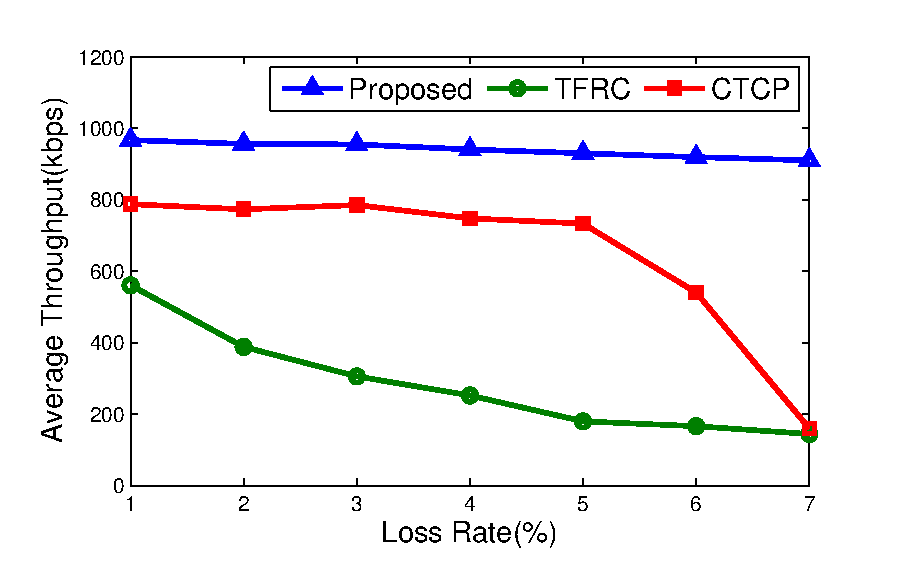
\includegraphics[scale=0.5]{lossrate_bw.eps}
            \caption{平均码率表现}
            \label{pic:lossrate_bw}
          \end{subfigure}
          \begin{subfigure}[b]{0.5\textwidth}
            \centering
            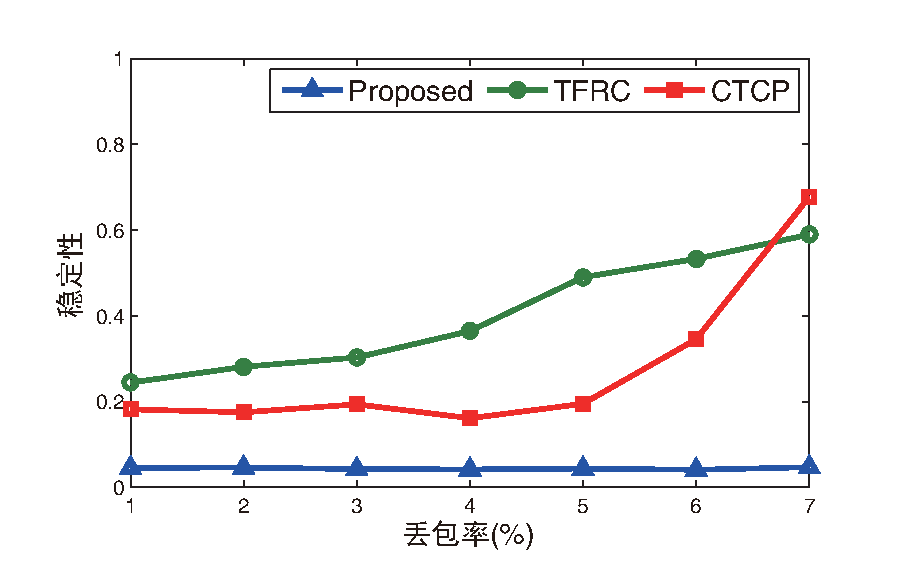
\includegraphics[scale=0.5]{lossrate_st.eps}
            \caption{码率稳定性表现}
            \label{pic:lossrate_st}
          \end{subfigure}
          \caption{不同丢包率下算法表现,带宽=1Mbps,背景延迟=50ms}
          \label{pic:lossrate}
        \end{figure}

        我们首先对平均码率和码率稳定性在不同算法间进行测试。图\ref{pic:lossrate}展示了不同丢包率的网络场景。可以看出我们的算法始终具有更好的表现。这主要由于我们的算法使用排队延迟而不是丢包作为网络拥塞信号,使其能够排除网络固有丢包对拥塞判断的影响。另外得益于控制论参数优化,尽管丢包率不断增大,我们的算法仍保持了较好的平均码率和码率稳定性水平。

        \begin{figure}[htbp]
          \begin{subfigure}[b]{0.5\textwidth}
            \centering
            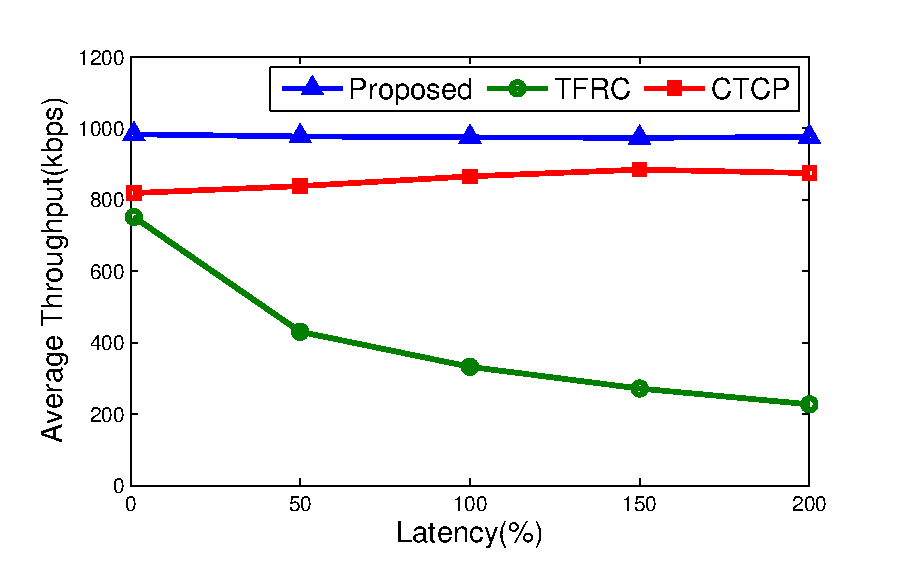
\includegraphics[scale=0.5]{latency_bw.eps}
            \caption{平均码率表现}
            \label{pic:latency_bw}
          \end{subfigure}
          \begin{subfigure}[b]{0.5\textwidth}
            \centering
            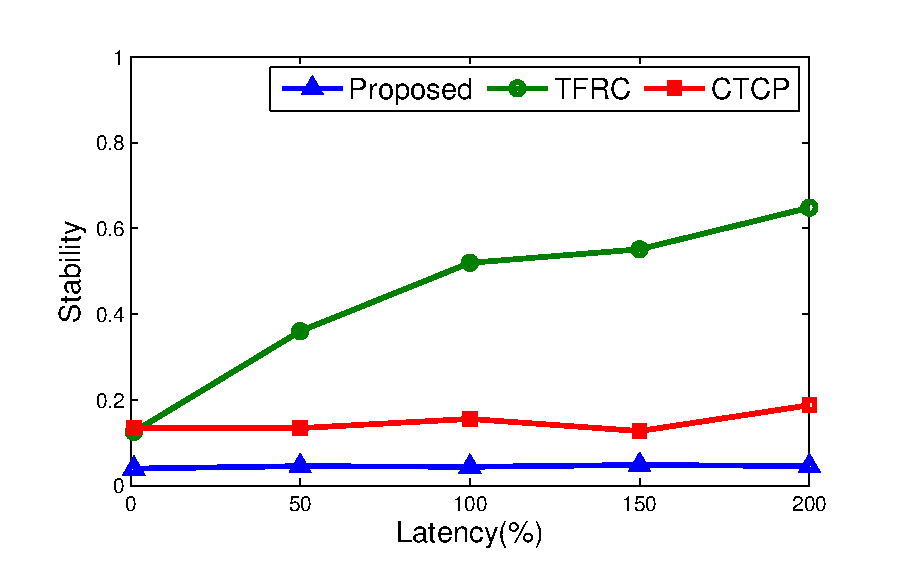
\includegraphics[scale=0.5]{latency_st.eps}
            \caption{码率稳定性表现}
            \label{pic:latency_st}
          \end{subfigure}
          \caption{不同背景延迟下算法表现,带宽=1Mbps,丢包率=1\%}
          \label{pic:latency}
        \end{figure}

        同时,我们比较了不同背景延迟条件下几种算法的表现,结果如图\ref{pic:latency}。从结果中可以看到,当延迟水平比较低时,所有算法都能得到较大的平均码率,随着延迟增大,基于延迟进行控制的TFRC算法平均码率急剧下降,而CTCP算法由于不考虑延迟变化,因此不受影响。我们的算法通过延迟优化,始终能保持较高的平均码率和较好的码率稳定性。

        \begin{figure}[htbp]
          \begin{subfigure}[b]{0.5\textwidth}
            \centering
            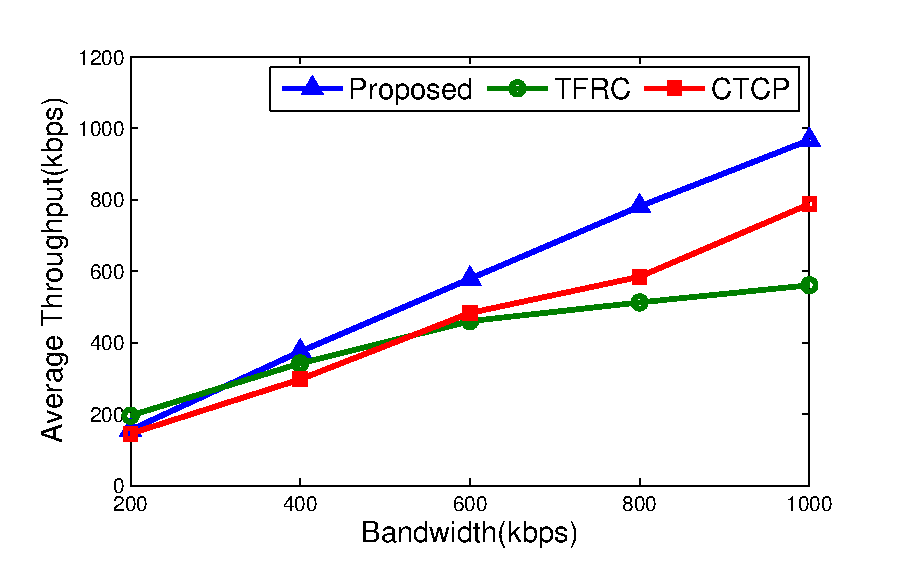
\includegraphics[scale=0.5]{bandwidth_bw.eps}
            \caption{平均码率表现}
            \label{pic:bandwidth_bw}
          \end{subfigure}
          \begin{subfigure}[b]{0.5\textwidth}
            \centering
            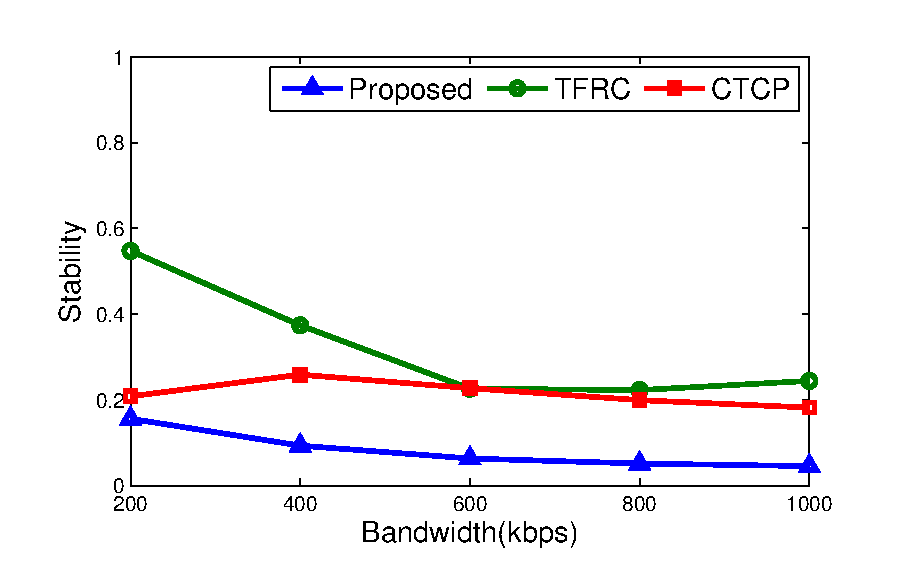
\includegraphics[scale=0.5]{bandwidth_st.eps}
            \caption{码率稳定性表现}
            \label{pic:bandwidth_st}
          \end{subfigure}
          \caption{不同带宽限制下算法表现,丢包率=1\%,背景延迟=50ms}
          \label{pic:bandwidth}
        \end{figure}

        最后,我们比较了不同网络带宽限制下几种算法的表现,如图 \ref{pic:bandwidth}。与前几项实验结果相同,我们的算法在不同环境中均表现出更好的效果。由于我们采用了排队延迟作为码率调整的主要信号,因而可以提前发现网络状况的波动,并通过改变码率来逼近实际带宽。另外得益于我们利用控制论进行的参数优化,保证了我们的码率自适应算法过程更加平滑、结果更加准确。

        \subsubsection{动态公平性}
        \begin{figure}[htbp]
          \centering
          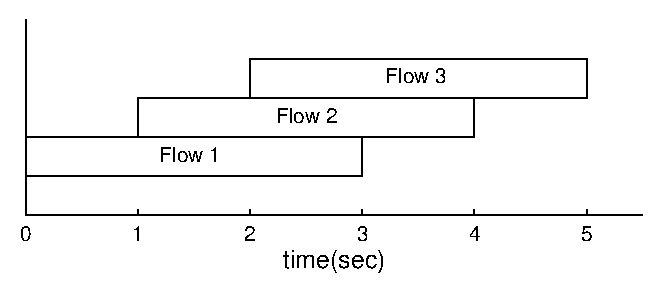
\includegraphics[width=0.5\textwidth]{flows.eps}
          \caption{多流动态模型}
          \label{pic:flows}
        \end{figure}
        \begin{figure}[htbp]
          \centering
          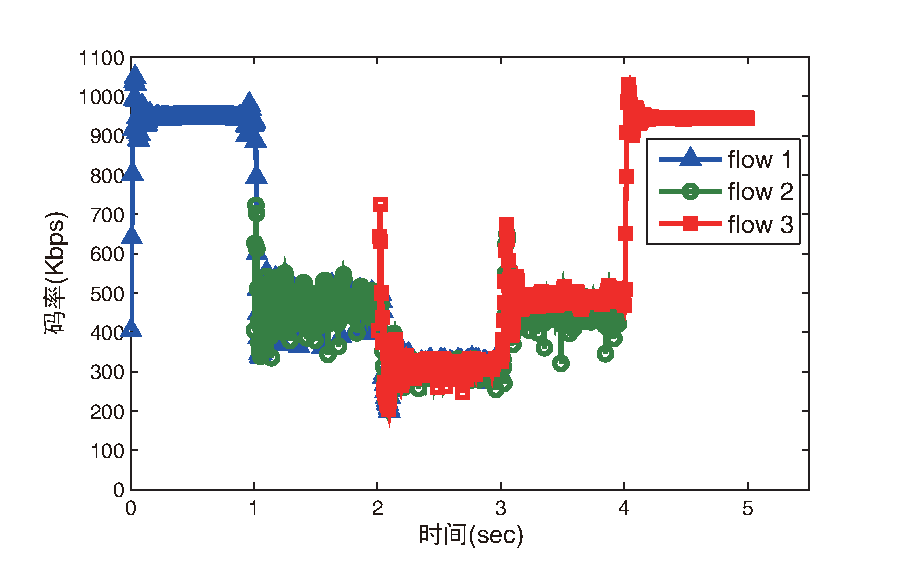
\includegraphics[width=0.7\textwidth]{flows_bw.eps}
          \caption{动态码率变化}
          \label{pic:flows_bw}
        \end{figure}

        除了静态网络中的测试以外,码率自适应算法在动态网络中能否迅速反应带宽变化也是评价的重要标准。本项测试中,我们选择三条数据流分别在不同时间启动和终止,如图\ref{pic:flows} 所示。在发送端,我们记录每条流的动态视频码率,结果如图\ref{pic:flows_bw}。 结果表明,我们的算法对网络波动反应迅速准确,并且每条流都能获取的均等大小的网络带宽。

        \subsubsection{视频质量}
        \begin{figure}[htbp]
          \centering
          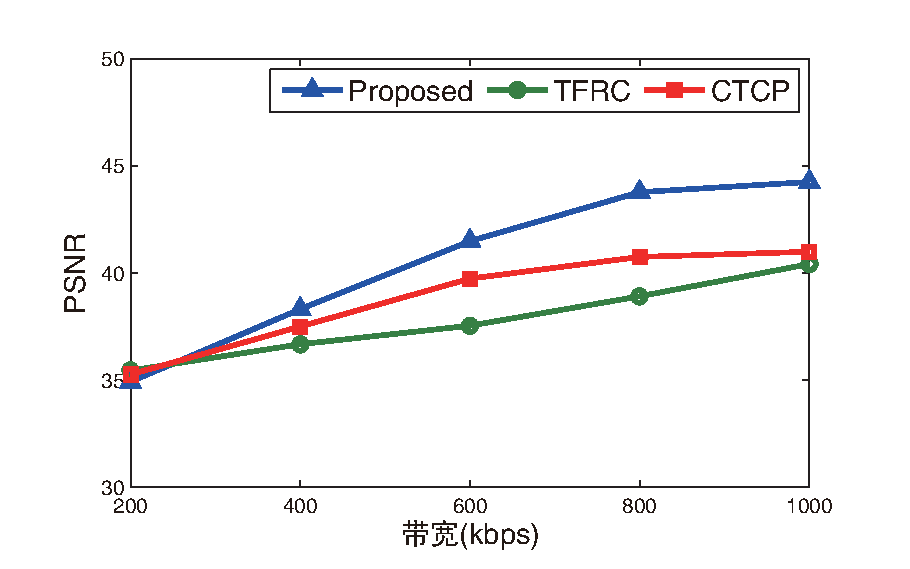
\includegraphics[width=0.7\textwidth]{psnr.eps}
          \caption{不同带宽限制下视频质量表现,丢包率=1\%,延迟=50ms}
          \label{pic:psnr}
        \end{figure}

        最后,我们比较了不同带宽限制下,三种码率自适应算法在接收端视频的PSNR质量表现,结果如图\ref{pic:psnr}所示。可见我们的算法在不同带宽下均能获得视频质量的显著提升。这主要得益于我们使用的比例控制器优化,及基于排队模型的延迟优化,使其能够获得更高的平均码率和码率稳定性。


\section{本章小结}
本章中,我们针对无线网络中的实时视频传输,提出了一个分布式、延迟可控的码率自适应算法,满足了视频传输中的低延迟、带宽稳定、高带宽利用率等需求。我们首先通过对网络建模分析,提出了简化网络链路的排队延迟模型,并引入了影子价格和失真权重参数来更好地实现拥塞控制和多流公平。通过建立闭环反馈控制模型,并引入比例控制器进行参数优化,使得控制过程更加高效、平滑。另外,我们在开源系统的基础上对几种码率自适应算法进行实现,并进行了大量效果测试。实验表明,相比于其他主流码率自适应算法,我们的算法在带宽利用率、稳定性,视频质量等方面都有更好的表现。

% !Mode:: "TeX:UTF-8"
% 文字编码:UTF-8
\chapter{基于非对称差错保护的冗余分配优化算法}
\label{chap:fec}

\section{引言}
第 \ref{chap:intro}章中已经提到,移动互联网正在成为网络发展的趋势,占据了越来越多的网络流量。而我们的视频通话系统也定位于为家庭Wi-Fi覆盖下的电视盒子以及移动电话等不同平台提供视频传输服务。由于无线网络不稳定,丢包率较高的特点,如果不采取措施改善丢包,视频画面将不可避免地出现卡顿、马赛克等,对用户体验造成影响。
在此背景下,我们必须为系统添加差错保护模块。
另一方面,实时视频传输对延迟的高度敏感,使得大部分成熟的差错保护算法都不能直接使用,如主动丢包重传、基于大编码块的FEC编码等,这些算法都会引入额外延迟。这也要求我们的视频通话系统针对网络状况进行差错保护算法优化。

在第 \ref{section:fec_intro} 节我们介绍了实时视频传输中常用的FEC算法,以及在编解码效果、额外延迟、非对称差错保护等方面的权衡和优化。在这些方法中,基于扩展窗口的RS编码 \cite{sejdinovic2009expanding} 表现出更多适合实时视频传输的优点:
\begin{itemize}
    \item 在每个GOP中,编码窗口不断扩展,编码块大小随之累积增加,从而在FEC编解码效率方面能得到较好的保障。
    \item 所有视频帧的编解码过程都只参考了当前和更早的视频帧,没有引入额外的编解码延迟。
    \item 越往前的视频帧,涉及到的编码块也越多,因而受到更多的冗余保护。这一特性恰好在一定程度上满足了视频数据非对称差错保护的要求。
\end{itemize}

但是在应用过程中,这一框架也存在一些问题,主要体现在:由于冗余分配优化问题复杂度很高,这一扩展窗口框架都采用了平均分配冗余的方案,并没有达到最高效率的冗余数据利用。在之前的分析中我们已经知道冗余分配主要以整个GOP的失真最小化为目标,这一过程需要求解每个视频帧在FEC编码后的丢包概率,而在扩展窗口框架下,视频帧的解码概率是非常复杂的,这也使得非对称差错保护在扩展窗口框架很难得到有效利用。

在本研究中,我们主要关注基于扩展窗口的FEC编码框架中,进行非对称差错保护并优化其效果的问题。首先,我们引入一种基于扩展窗口的Reed-Solomon编码框架并对其进行数学建模分析,提出其成功解码的充要条件。通过对编解码模型的分析并引入等效模型简化计算,我们得到了视频帧丢帧概率模型。结合视频帧对整体失真的影响大小,可以得到非对称保护中最关键的失真优化问题。最后我们通过简化的贪心算法解决了这一优化问题,得到GOP 中的最优冗余分配方案,达到更好的非对称差错保护效果。实验表明,我们的算法在各种网络条件下,都能显著提高受保护视频的PSNR表现。


\section{基于扩展窗口的FEC冗余分配}
在数据不可靠的网络中,FEC是一种有效的检错、纠错方法。然而,在FEC的保护效果和引入的额外延迟之间一直存在妥协:编码块越大,编码效率越高,额外延迟也越大;编码块越小,额外延迟越小,而编码效率也越低。在延迟敏感的实时视频传输中,这一问题变得更加突出。

为了平衡编码效率和延迟之间的矛盾,我们采用了图 \ref{fig:ew_fec} 所示的扩展窗口RS编码框架(EW-RS)。 在发送端,每一视频帧与同一GOP 中所有之前的视频帧数据同时编码。在接收端,奇偶校验方程包含了所有GOP 中之前的数据,并求解出丢失的数据包。由于后续视频帧的校验码中都包含了之前视频帧的数据信息,可以用于回复前面丢失的数据包,这也在一定程度上实现了非对称差错保护。同时由于所有编解码都只引用了当前和之前的数据包,因此整个过程不会引入额外延迟。

由于这一框架的编码块层层嵌套,添加冗余后各视频帧在丢包情况下解码概率的提升程度很难被准确计算,因而也无法套用常规的非对称差错保护分析框架进行冗余分配。接下来我们会通过一系列变换和简化解决这一问题,推导出最优冗余分配方案。

    \subsection{EW-RS 框架下的丢包率计算}
    对于一个GOP,假设其包含$N$个视频帧,其中第$n$帧的数据包和相应校验包数量分别记为$k_n$和$r_n$。我们采用的Reed-Solomon编码可以表示为一个$RS(\hat{N},\hat{K})$ \cite{wicker1999reed} 系统,其中$\hat{N}$是编码块大小,$\hat{K}$是编码块中的源数据包数量。接收端能够成功解码该编码块的条件是,接收到任意源数据包或校验包的总数量大于$\hat{K}$。针对我们采用的扩展窗口框架,某一视频帧$n$的解码条件为:
    \begin{equation}\label{eq:gf-2}
      \left\{ \begin{array}{l}
        \mathbf{A_{1}}\mathbf{X_1} = \mathbf{C_1}\\
        \mathbf{A_{2}}(\mathbf{X_1}^T, \mathbf{X_2}^T)^T= \mathbf{C_2}\\
        \cdots\\
        \mathbf{A_{n}}(\mathbf{X_1}^T,\mathbf{X_2}^T,\cdots,\mathbf{X_{n}}^T)^T = \mathbf{C_{n}}\\
      \end{array} \right.
    \end{equation}
    其中$\mathbf{X_i}=(x_{i,1},x_{i,2},\cdots,x_{i,k_i})^T$ 是$k_i \times 1$向量,代表第$i$视频帧的所有源数据包;$\mathbf{C_i}=(c_{i,1},c_{i,2},\cdots,c_{i,r_i})^T$ 是$r_i \times 1$向量,代表第$i$视频帧的所有校验包。
    每个丢失的数据包都对应$X_i$(源数据包)或 $C_i$ (校验包)中的一个变量。
    $\mathbf{A_i}$是$r_i \times \sum_{j=1}^{i}k_j$矩阵,代表第$i$帧对应编码块的奇偶校验矩阵。
    注意到变量$\mathbf{X_i}$包含在序号为$j,\; j \le i$ 的所有校验方程中,因此每个编码窗口的解码过程都包含了对GOP中之前数据包的解码,从而使前面的数据包具有更大的解码概率。
    这里需要注意的是,根据基本代数知识,方程组能够求解的充要条件是系数矩阵的秩不小于未知数的个数,这就要求系数矩阵$\mathbf{A_{i}}, \forall i \in [1,n]$不存在共线性。在Xiao \cite{xiao2013real}的方法中,通过对系数矩阵$\mathbf{A_{i}}$进行随机化,基本保证了式\ref{eq:gf-2}中的方程组为满秩。

    为了得到每一视频帧的丢帧概率,我们首先对式\ref{eq:gf-2}进行分析,并总结出与数据包解码相关的两条基本命题如下:

    \begin{corollary}\label{th:1}
    在EW-RS框架中,如果第$n$个视频帧能够解码,那么同一GOP中所有之前的视频帧也都能够解码。
    \end{corollary}

    \begin{proof}
    根据图\ref{fig:ew_fec}和式\ref{eq:gf-2},第$n$视频帧的校验包对应的编码块包含了所有当前和之前帧的数据包,第$n$帧解码对应了该编码块成功解码,这也就意味着所有数据包都能够解码。
    \end{proof}

    \begin{corollary}\label{th:2}
    记$l_i$为第$i$视频帧丢失数据包的数量,那么视频帧$n$成功解码的充要条件为:
     \begin{equation*}
      \left\{ \begin{array}{ll}
        l_n \le r_n\\
        l_{n-1} + l_n \le r_{n-1} + r_n\\
        \cdots\\
        \sum_{j=1}^{n}l_j \le \sum_{j=1}^{n}r_j
      \end{array} \right.
    \end{equation*}
    \end{corollary}

    \begin{proof}
    我们使用反证法证明此推论。对于上式中的约束,假设存在$k$使得$\sum_{i=k}^{n}l_i > \sum_{i=k}^{n}r_i$,同时视频帧$n$仍然能够成功解码。记第$k$到$n$ 帧的所有奇偶校验方程组成子方程组$\mathcal{E}$,则该方程组的秩为$\sum_{i=k}^{n}r_i$,即帧$k$ 到 $n$的所有校验包的数量。根据推论\ref{th:1}可知,此时GOP中$1$到$n$的所有视频帧均能够成功解码。那么对于方程组$\mathcal{E}$,其未知数数量为$\sum_{i=k}^{n}l_i$大于方程组的秩,这与方程组求解条件矛盾。
    \end{proof}

    推论\ref{th:1}表明如果某一视频帧能够解码,其同一GOP中所有之前的视频帧都能够解码,因此GOP序列中视频帧间的依赖被消除。推论\ref{th:2}给出了某一视频帧能够成功解码的充要条件。为了达到优化冗余分配的目的,我们必须定量分析每一视频帧在FEC编码条件下的解码概率,而推论 \ref{th:2} 给出的解码条件包含复杂的嵌套关系,显然无法满足正常复杂度下的求解。尽管如此,我们还是通过迭代的形式给出视频帧$n$解码概率的公示表示如下
    \begin{equation}\label{eq:ep_nth}
        P(n) = 1 - \sum_{i=0}^{ r_{n} } (\mathcal{F}(k_{n}+r_{n}, i, p) \sum_{j=0}^{ r_{n} - i } \mathcal{F}(\sum_{z=1}^{n-1}k_z, j, \overline{P}(n-1)))
    \end{equation}
    其中$\mathcal{F}(a, b, c)={a \choose b} c^{b} (1-c)^{a-b}$是二项式概率密度函数,$p$代表信道数据传输的错误率(丢包率)。

    在扩展窗口框架下,不同帧对应的数据包具有不同的丢包概率,这是造成视频帧解码概率求解困难的主要原因。为了简化计算,我们在迭代计算过程中,近似认为所有已经完成求解的数据包丢包概率相等,并用一个等效丢包概率对其进行近似。对于第$1$ 到 $n-1$ 帧,其等效丢包概率定义为$\overline{P}(n-1)$,根据定义,用$\overline{P}(n-1)$或$P(n-1)$ 求得的所有数据包的解码的概率应该相等,即
    \begin{equation}\label{eq:eq}
    (1 - \overline{P}(n-1))^{\sum_{i=1}^{n-1}k_i} = 1 - P(n-1)
    \end{equation}
    其中等号左边表示用等效丢包概率计算所有数据包都能解码的概率,等号右边表示第$n-1$帧视频帧能够解码(也即所有数据包都能解码)的概率。

    有了递推公式 \ref{eq:eq},我们就可以从GOP的第一帧开始,通过递推求得每一视频帧的解码概率。第一帧视频帧的等效丢包概率可以用式 \ref{eq:ep_nth}这一原始形式求解,即初始值$P(1)$为
    \begin{equation}\label{eq:first_packet}
    P(1) = 1 - \sum_{i=0}^{r_1} \mathcal{F}(k_1+r_1, i, p)
    \end{equation}


    \subsection{视频传输失真优化模型}
    一般来说,由于视频编码过程中的帧间压缩技术,视频帧之间互相参考,某一视频帧的丢失会造成GOP 中后续视频帧的失真。一个极端的例子是,如果GOP中的I帧丢失,则所有后续视频帧都将无法解码。在本研究的框架中,根据推论 \ref{th:1},只要当前帧能够解码,则GOP中所有之前帧也都已经成功解码,通过参考缓冲区更新技术,可以保证解码过程中不存在错误传播。

    在基于手机、电视盒子等智能设备的实时视频通话系统中,由于计算能力的限制,对于视频帧解码失败的处理一般都比较简单,最常见的是直接保持上一帧成功解码视频帧的画面。为了量化视频帧丢失对画面质量的影响,一般对原始视频和处理后视频计算PSNR作为视频失真的度量。在本模型中,我们假设一帧丢失后,复用前一帧的画面,并以此计算丢包前后该视频帧的PSNR,代表当前帧无法播放对GOP整体失真的贡献。记第$n$帧的PSNR为$\gamma(n)$,考虑到前述该帧的丢包率为$P(n)$,可以计算其预期失真
    \begin{equation}\label{eq:distortion}
      D(n)=\gamma(n)P(n)
    \end{equation}
    对于整个GOP,其预期失真定义为GOP中所有视频帧预期失真的加和,即
    \begin{equation}\label{eq:t_dist}
    \overline{\mathcal{D}} = \sum_{i=1}^{N}D(n)
    \end{equation}

\section{问题建模和优化求解}
前文已经分析了已知GOP中各视频帧失真度量和丢帧率前提下,整个GOP预期失真的计算。我们知道,即使采用相同的FEC编码冗余率,冗余信息的不同分配方式也会对保护效果产生很大影响,根据这一效果差异进行冗余信息的最优分配也就是通常的非对称差错保护。
为了提升本研究中的FEC冗余保护效果,我们希望找到一种能够使GOP整体预期失真最小的冗余分配方案。
结合式 \ref{eq:eq}和 \ref{eq:t_dist},这一冗余信息分配问题可以抽象为一个带约束的线性优化问题:
\begin{equation}
\label{eq:lp1}
\begin{aligned}
& \mathbf{r}^{*} =
& & \underset{\mathbf{r}}{\arg\min} \overline{\mathcal{D}}(\mathbf{r}) \\
& \text{s.t.}
& & \sum_{i=1}^{N}(k_i + r_i) \le C \\
&&& r_i \ge 0, \forall i \in [1,N]. &{} &
\end{aligned}
\end{equation}
其中$C$表示网络带宽上限。约束一限制了所有源数据包和冗余数据包的数量上限,这一上限值与网络带宽以及系统设定有关。而约束二要求所有编码块的冗余信息量都不能为负。

这一带约束优化问题的目标是找到使整体预期失真最小的冗余分配方案$\mathbf{r}^{*}$,从而最大化非对称差错保护的效果。在式\ref{eq:lp1}的非线性整数优化问题中,通过穷举法得到最优解的时间复杂度为$N^{R}$(这里$R$代表所有校验包数量的最大值),其计算量是实时系统所无法容忍的。

\begin{algorithm}[htbp]
\caption{式\ref{eq:lp1}的次优贪心解法}
\label{al:hc}
    \begin{algorithmic}
    \State $\mathbf{r}, \mathbf{r}^{*} \gets (0,\cdots,0)$
    \State $\overline{\mathcal{D}} \gets +\infty$
    \For{$i \gets 1,R$}
        \State $\mathbf{r} \gets \mathbf{r}^{*}$
        \For{$j \gets 1,N$}
            \State $r_j \gets r_j + 1$
            \State $\overline{\mathcal{D}}_{t} \gets \overline{\mathcal{D}}(\mathbf{r})$
            \If{$\overline{\mathcal{D}}_{t} < \overline{\mathcal{D}}$}
                \State $\overline{\mathcal{D}} \gets \overline{\mathcal{D}}_{t}$
                \State $\mathbf{r}^{*} \gets \mathbf{r}$
            \EndIf
            \State $r_j \gets r_j - 1$
        \EndFor
    \EndFor
    \end{algorithmic}
\end{algorithm}

为了解决这一计算复杂度问题,我们提出了一个基于贪心算法的次优解法,见算法 \ref{al:hc}。该算法中,我们将校验包逐个分配到整个GOP的编码块中,对于每个校验包,都逐一测试所有编码块,并最终确定在能使当前整体预期失真最小的编码块。这一算法的复杂度降低到$\mathcal{O}(NR)$,并且实验表明,其结果与穷举整个解空间得到的结果基本相同。
这一算法得到的向量$\mathbf{r}^{*}$即可直接用于GOP扩展窗口编码过程中的冗余数据包分配。

\section{实验验证}
本小节,我们通过模拟实验测试了我们提出的算法的性能,并与原始算法进行了对比。

    \subsection{实验设置}
    本研究使用的RS编码属于$(N,K)$编码的一种,其解码与否只取决于收到的数据包数量是否不小于$K$,这一性质使我们可以大大简化实验流程。我们不需要完全重现视频数据的采集、编码、FEC编码、网络丢包模拟、FEC解码、视频解码和播放这一系列步骤,而只需要生成代表数据包是否丢失的二值序列(如0代表丢包,1代表成功接收),在接收端统计收到数据包的数量与$K$的关系即可决定能否解码。这一系列过程都可以在Matlab中完成。

    具体来说,我们通过Matlab调用JM18 \cite{website:jm18}和H.264/AVC \cite{zhang2000video} 编解码库完成视频文件到视频数据包的转换。对于生成的数据包序列,一个随机函数根据指定的丢包率随机将其中一部分包标记为丢失。在RS解码函数中,通过统计接收到的冗余包和源码包数量是否满足解码条件判断能否恢复丢失的数据包。最后数据包在Matlab中完成解码和PSNR的计算。

    我们选择了Foreman, Bus, Mobile 和 Stefan 四个不同风格的视频序列作为我们实验的视频源。视频编码后,GOP为IPPP形式、大小为30 帧,并且根据不同带宽设置选择视频压缩率。每一帧编码产生的数据流根据网络MTU 进行分包封装,生成一系列的视频数据包。

    为了对比本文提出的算法改进能否取得明显的性能提升,我们选择了本改进算法的基础:扩展窗口的RS编码(EW-RS)\cite{xiao2013real},以及最原始的平均分配冗余的FEC编码算法作为对照。
    EW-RS算法采用了前述扩展窗口的FEC编码框架,在不引入额外延迟的前提下大大提高了编码块规模,因而提高了编解码效率。然而文章中采用了平均分配冗余包的方法,对于不同特性的视频以及不同丢包率的网络不具有适应性。
    平均分配冗余的FEC编码算法作为最原始的差错保护算法,往往需要较大的编码块以保证编解码效率,因此引入较大的额外延迟,另外冗余包的分配方式同样没有考虑到视频的非对称特性。

    \subsection{结果分析}

\begin{figure}[htbp]
  \centering
  % Requires \usepackage{graphicx}
  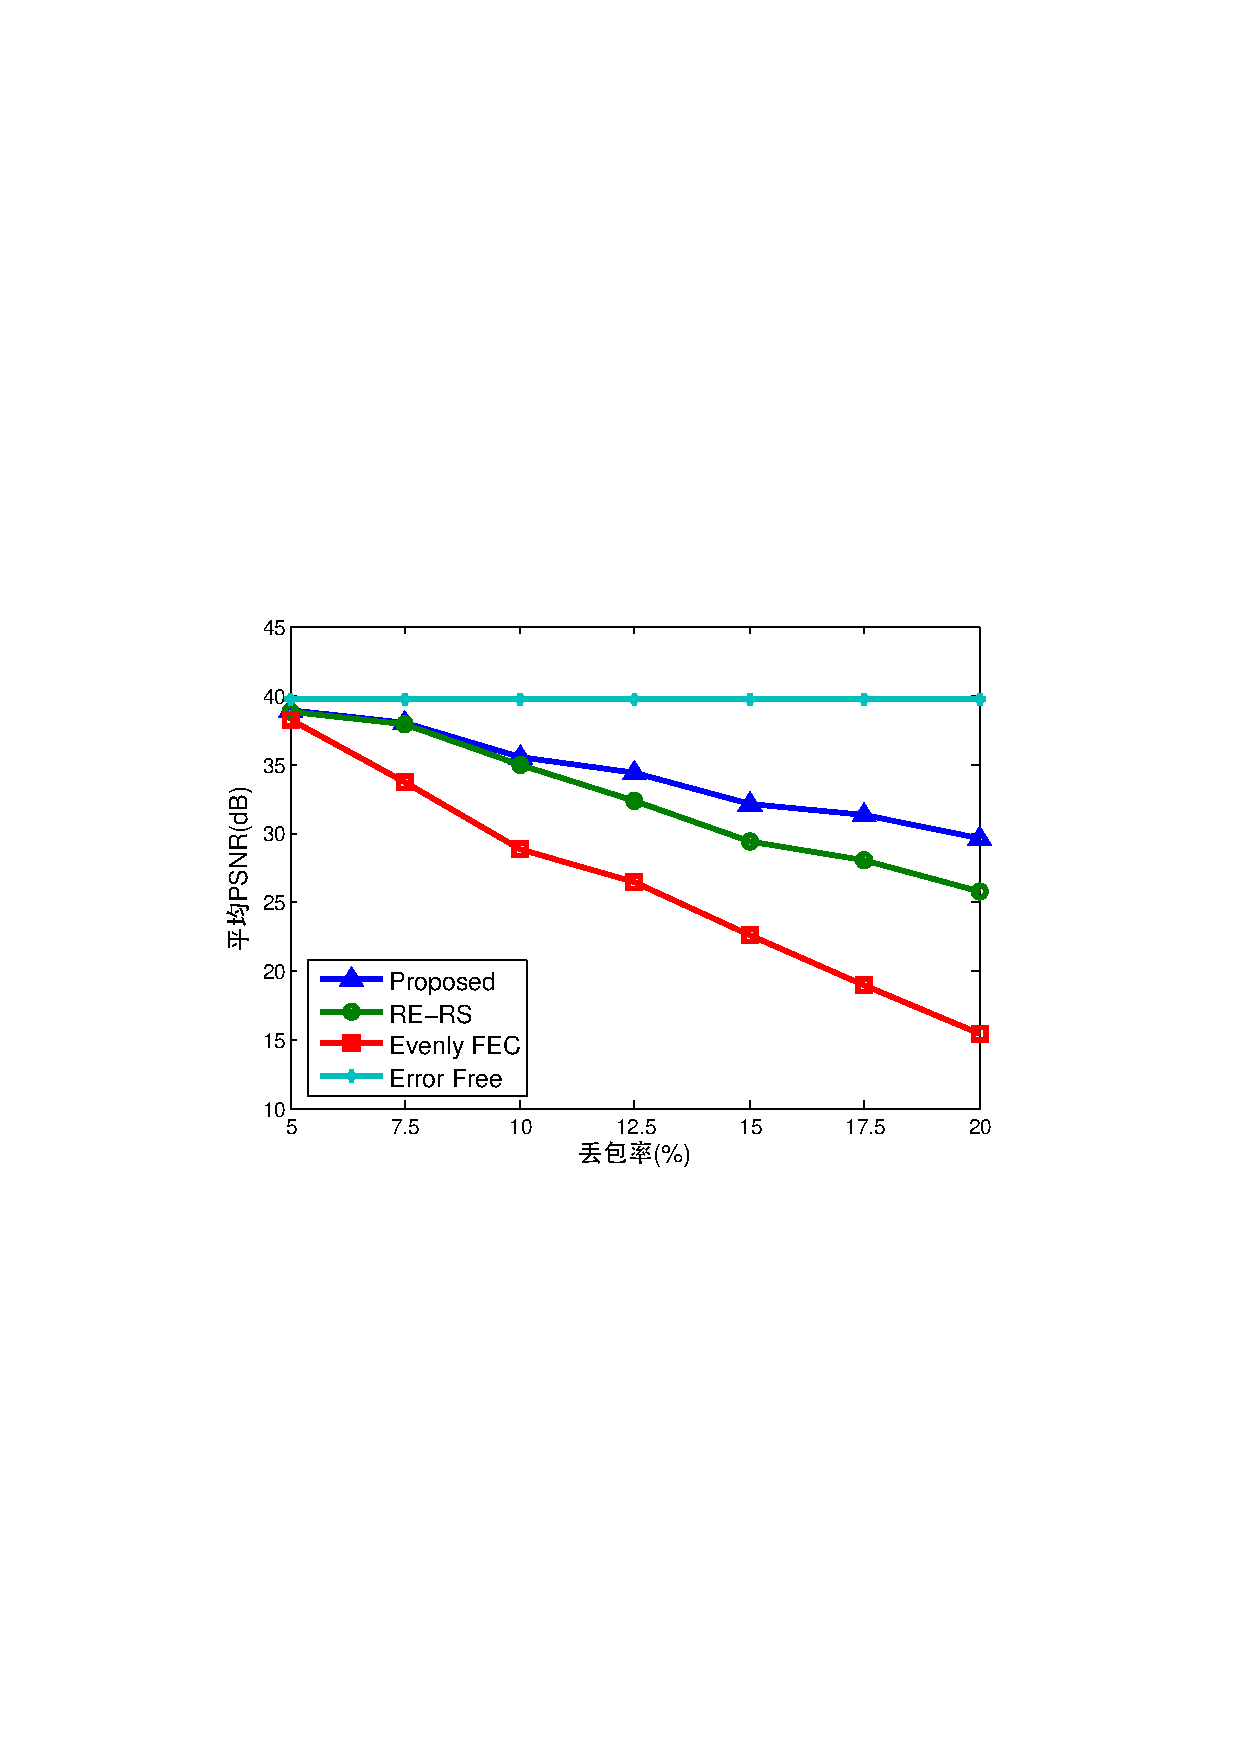
\includegraphics[width=0.7\textwidth]{uep_loss_rate.pdf}\\
  \caption{不同丢包率下PSNR表现,带宽=1Mbps,871 Kbps \emph{Foreman}序列}\label{fig:lossrate}
\end{figure}

首先,我们比较了上述三种算法在不同丢包率环境下的PSNR表现。在本实验中,我们使用了编码码率为871Kbps的\emph{Foreman}序列,网络带宽限制为1M。实验结果如图\ref{fig:lossrate}所示,其中无丢包情况的PSNR表现作为基准值标出。图中可以明显看出,我们的算法在所有丢包率情况下PSNR表现都高于其他算法,值得注意的是,随着丢包率的增大,这一差距也越来越明显。这一效果提升得益于我们的算法在不同丢包率场景下,能够通过理论计算得到最优冗余分配方案,在相同冗余率下获得更好的保护效果。当丢包率达到$20\%$时,我们的算法相比RE-RS算法获得了高达5.0 dB的PSNR增益。

\begin{figure}[htbp]
  \centering
  % Requires \usepackage{graphicx}
  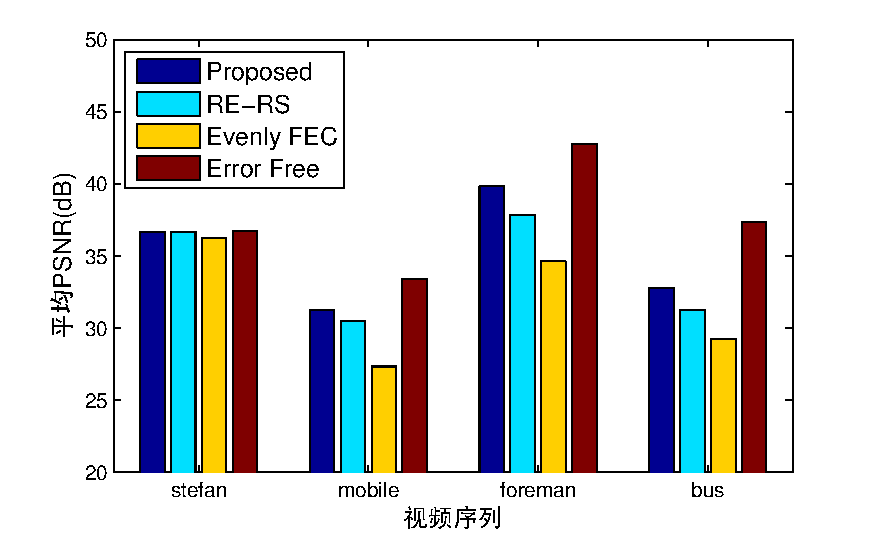
\includegraphics[width=0.7\textwidth]{videos.pdf}\\
  \caption{不同视频序列下PSNR表现,带宽=2Mbps,序列:\emph{Stefan}:1441Kbps, \emph{Mobile}:1786Kbps, \emph{Foreman}:1812Kbps, \emph{Bus}:1890Kbps}\label{fig:videos}
\end{figure}

为了测试算法对不同特征视频的适应性,我们还用不同特点和码率的视频序列对三种算法的表现进行了实验。图 \ref{fig:videos} 表明,我们的算法在不同视频序列中均表现出更好的冗余保护效果。并且随着视频码率提高(同带宽下冗余率相应降低),我们的算法由于能够更有效地利用有限的冗余数据,因而获得了更明显的效果提升。

\begin{figure}[htbp]
  \centering
  % Requires \usepackage{graphicx}
  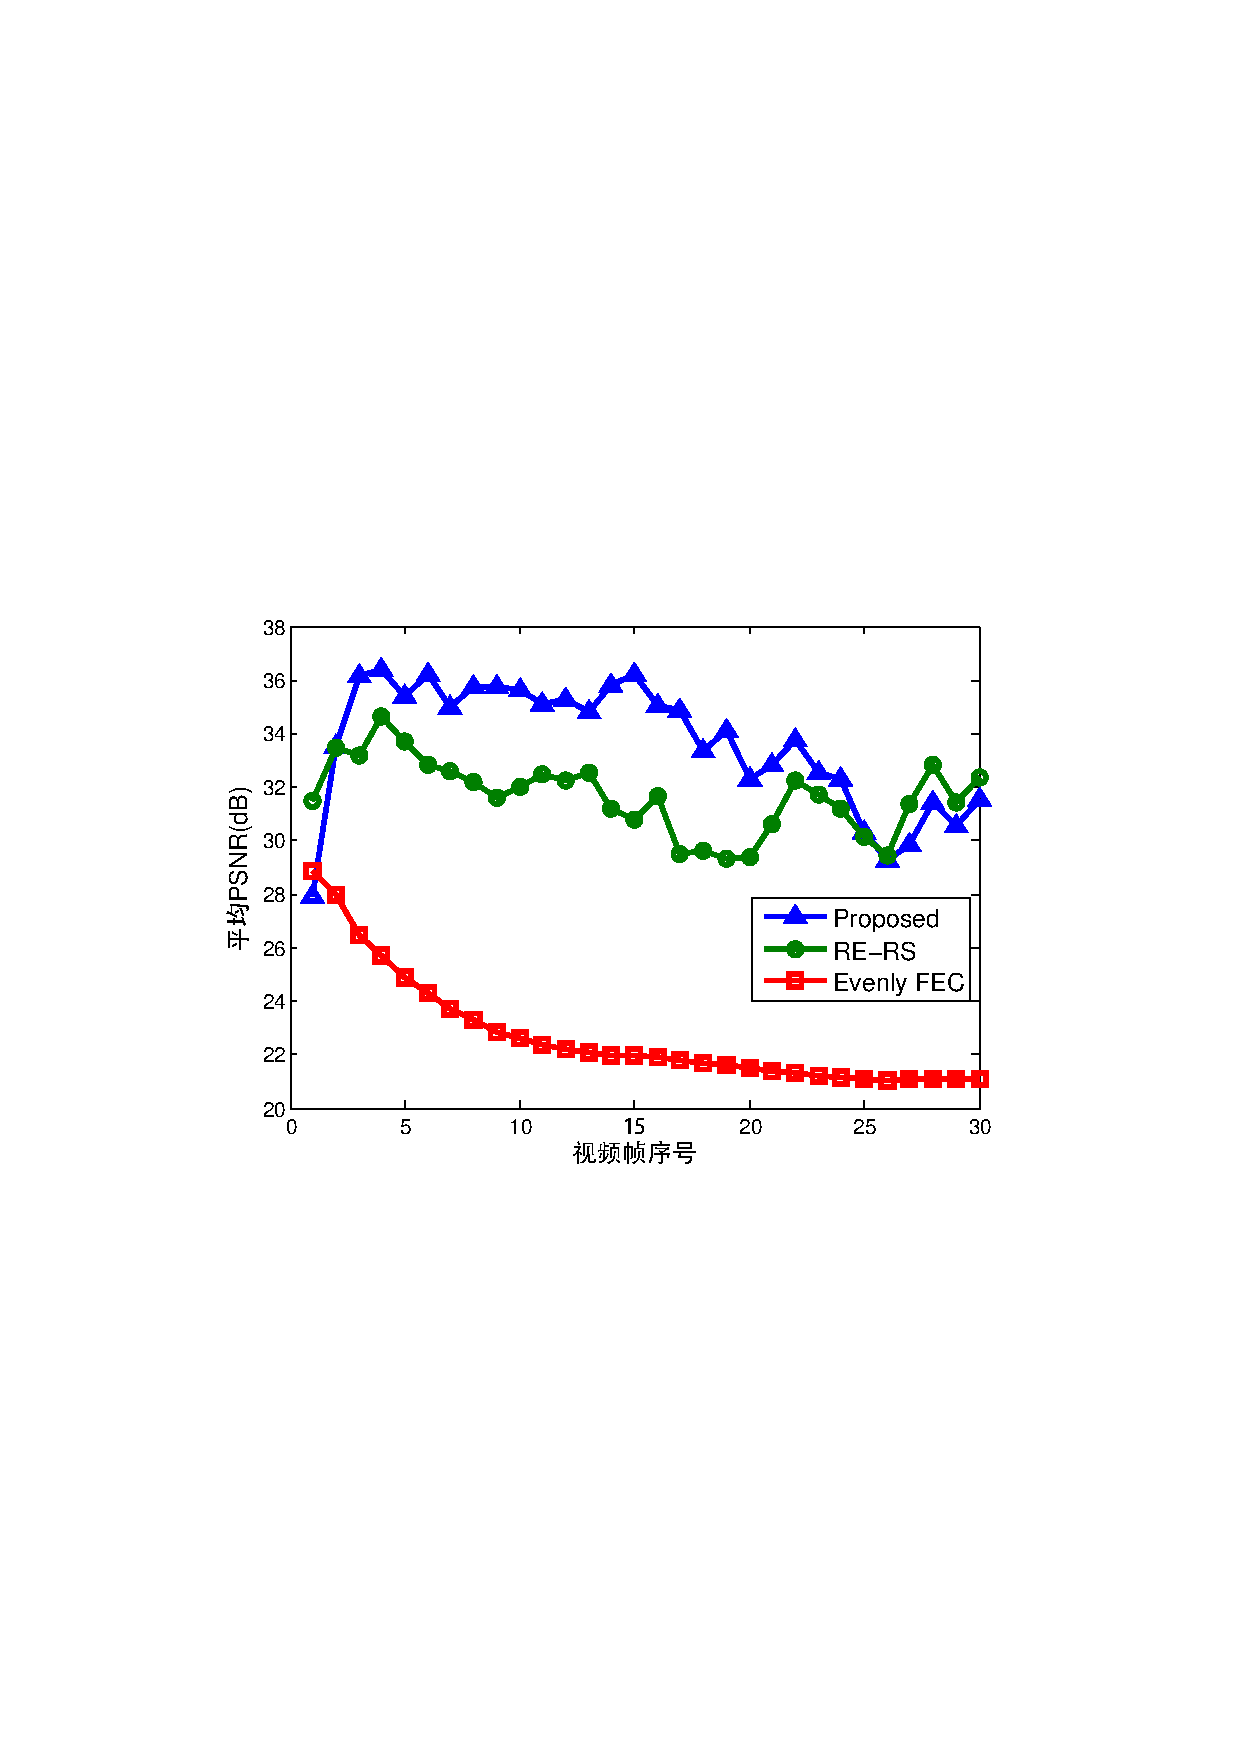
\includegraphics[width=0.7\textwidth]{uep_psnr.pdf}
  \caption{逐帧PSNR表现,丢包率=$10\%$,带宽=1Mbps,871 Kbps \emph{Foreman}序列}\label{fig:psnr}
\end{figure}

最后,为了分析我们的算法在FEC冗余优化分配中的具体原理,我们对\emph{Foreman}序列在10\%丢包率,1Mbps带宽条件下进行了测试,并绘制了三种算法在GOP中每一帧的PSNR表现,如图\ref{fig:psnr}。在RE-RS和我们的算法中,由于采用了扩展窗口编码框架,视频帧间的错误传播都得到了有效控制,因此不会出现Evenly FEC这种随着帧序列增大失真明显增多的现象。而我们的算法通过在不同帧之间冗余信息的优化分配,达到了整体上失真的最小化。


\section{本章小结}
本研究中,我们对一种针对实时视频传输的扩展窗口FEC框架进行了建模、分析,并提出了一种基于此框架的冗余分配方案。我们首先针对EW-RS框架进行了准确的丢包率分析,并针对其编解码特征提出了两条推论。然后我们推导出了GOP整体语预期失真公式,作为冗余最优化分配的理论基础。在此基础上,冗余分配问题被归纳为带约束的非线性优化问题。另外,为了简化这一问题的求解,我们设计了一种基于贪心的次优求解算法,使这一冗余分配算法能够适用于实时传输场景。大量实验结果表明,我们的算法在各种网络场景下都能明显提高视频传输的FEC保护效果。

% !Mode:: "TeX:UTF-8"
% 文字编码:UTF-8
\chapter{总结与展望}
\label{chap:conclusion}

\section{本文工作总结}
科技的进步不断改变人们的生活方式,给人们的生活带来便利,视频通话的兴起和发展就是一个很好的例证。当然任何技术的进步都离不开学术界和工业界的共同努力,视频通信服务的发展也并非一帆风顺。实时视频对丢包和延迟高度敏感以及要求较大且稳定的带宽,与无线网络质量多变、不可靠的传输环境相矛盾,给高质量的实时视频传输服务带来很大挑战。为了在无线网络下进行高质量的视频通话,可以从拥塞控制和差错控制两方面进行优化。针对动态的网络带宽,及时地调整传输视频的码率可以避免网络拥塞并最大化带宽利用率。另一方面,针对无线网络易丢包的特点以及实时视频对延迟的需求,采用FEC编码可以为视频流提供一定的抗丢包能力,获得更好的视频体验。
本文以无线网络全面覆盖、视频通话需求火热为背景,实现了一个针对无线网络环境特点、以家庭电视盒子为主要平台的高清视频通话应用,并针对上述两个方面分别进行了算法优化和系统实现,我们的贡献主要包括以下方面:
\begin{enumerate}
    \item 针对无线网络中的实时视频传输,我们提出了一个分布式、延迟可控的码率自适应算法,满足了视频传输中的低延迟、带宽稳定、高带宽利用率等需求。我们首先通过对网络建模分析,提出了简化网络链路的排队延迟模型,并引入了影子价格和失真权重参数来更好地实现拥塞控制和多流公平。通过建立闭环反馈控制模型,并引入比例控制器进行参数优化,使得控制过程更加高效、平滑。另外,我们实现了一套完整的算法测试平台,并对算法进行了系统实现和大量效果测试。实验表明,相比于其他主流码率自适应算法,我们的算法在带宽利用率、稳定性,视频质量等方面都有更好的表现。
    \item 我们对一种针对实时视频传输的扩展窗口FEC框架进行了建模、分析,并提出了一种基于此框架的冗余分配方案。我们首先针对EW-RS框架进行了准确的丢包率分析,并针对其编解码特征提出了两条推论。然后我们推导出了GOP整体语预期失真公式,作为冗余最优化分配的理论基础。在此基础上,冗余分配问题被归纳为带约束的非线性优化问题。另外,为了简化这一问题的求解,我们设计了一种基于贪心的次优求解算法,使这一冗余分配算法能够适用于实时传输场景。大量实验结果表明,我们的算法在各种网络场景下都能明显提高视频传输的FEC保护效果。
    \item 利用本文中算法方面的工作,我们基于开源软件对其内核进行了重写,实现了新的码率自适应和差错保护模块,实验表明这一新的底层模块大大改进了原软件的视频通话体验。为了充分发挥高质量视频传输的功能,我们还对其界面进行了优化,将其移至电视盒子上,从而实现了面向无线网络环境,电视机大屏幕上的高清视频通话。
\end{enumerate}


\section{未来工作展望}
在下一步的工作中,我们将继续深入实时视频传输过程中的拥塞控制和差错保护优化。尽管本文提出的算法已经在一定程度上改善了无线网络上实时视频传输的效果,但还远远无法满足日益增长的高清视频需求和日益多样化的网络环境。未来的工作可以从以下不同方面展开:
\begin{enumerate}
    \item 视频码率自适应算法可以参考的网络参数包括丢包率、延迟、抖动等,多数算法都只针对其中一个或几个方面进行了优化,却很难兼顾这些参数之间的关系及其对视频质量的系统性影响。例如只针对延迟进行调整,则算法在与基于丢包的算法竞争时存在饥饿现象;而只对网络丢包进行反应,则会造成网络延迟急剧增加。如何更好地综合各种网络参数,对网络状态进行估计进而控制视频码率,是下一步可以优化的问题之一。
    \item 视频马赛克、丢帧以及通话延迟等是公认影响视频通话用户体验的因素,然而还没有客观的标准定量地评价这些指标对用户体验的影响。这一方面给传输优化算法的比较带来困难,另一方面也不利于视频传输算法的进一步优化。因此在视频体验的定量评价方面也可以进行一些实验和研究。
    \item 在智能手机上进行FEC编解码会对其计算资源带来比较大的负载,引起发热、性能下降等问题。因此针对低性能的移动设备进行FEC编解码优化也是进一步提高实时视频通话体验的一种方法。
\end{enumerate}


%结论

%% !Mode:: "TeX:UTF-8"
% 文字编码:UTF-8
%%%%%%%%%%%%%%%%%%%%%%%%%%%%%%%%%%%%%%%%%%%%%%%%%%%%%%%%%%%%%%%%%%%%%%%%%
%
%   LaTeX File for Doctor (Master) Thesis of Peking University
%   LaTeX + CJK     北京大学博士(硕士)论文模板
%   Based on Wang Lei's Template for THU
%   Version: 1.00
%   Last Update: 2005-05-25
%
%%%%%%%%%%%%%%%%%%%%%%%%%%%%%%%%%%%%%%%%%%%%%%%%%%%%%%%%%%%%%%%%%%%%%%%%%
%   Copyright 2004-2005  by  Ying Pan       (yeying_pan@yahoo.com.cn)
%%%%%%%%%%%%%%%%%%%%%%%%%%%%%%%%%%%%%%%%%%%%%%%%%%%%%%%%%%%%%%%%%%%%%%%%%
%%%%%%%%%%%%%%%%%%%%%%%%%%%%%%%%%%%%%%%%%%%%%%%%%%%%%%%%%%%%%%%%%%%%%%%%%
%
%   LaTeX File for Doctor (Master) Thesis of Tsinghua University
%   LaTeX + CJK     清华大学博士(硕士)论文模板
%   Based on Wang Tianshu's Template for XJTU
%   Version: 1.00
%   Last Update: 2003-09-12
%
%%%%%%%%%%%%%%%%%%%%%%%%%%%%%%%%%%%%%%%%%%%%%%%%%%%%%%%%%%%%%%%%%%%%%%%%%
%   Copyright 2002-2003  by  Lei Wang (BaconChina)       (bcpub@sina.com)
%%%%%%%%%%%%%%%%%%%%%%%%%%%%%%%%%%%%%%%%%%%%%%%%%%%%%%%%%%%%%%%%%%%%%%%%%
\chapter{结论与展望}
%\markboth{结论}{结论}
%\addcontentsline{toc}{chapter}{结论}
\section{结论}


\section{展望}

\cleardoublepage

%\backmatter

%参考文献
\bibliographystyle{a01}
%\bibliographystyle{acm}  %张宏剑
%agsm是一种harvard的文献格式,%如果需要使用这种
%格式,要在setup/packages.tex中去掉\usepackage{harvard}的注释
%\bibliographystyle{agsm}

\phantomsection
\addcontentsline{toc}{chapter}{参考文献}

%\addtolength{\itemsep}{-0.8 em} % 缩小参考文献间的垂直间距, 在bibtex下无效
%\bibliographystyle{plain}
%\nocite{*}
{\typebib
%\setlength{\bibspacing}{\baselineskip}
\bibliography{body/COEreference}
}
%打印索引
%\generateindex
\cleardoublepage
%附录
%\begin{appendix}
%%   \renewcommand{\chaptername}{附录\Alph{chapter}}
%\renewcommand{\chaptermark}[1]{\markboth{附录\Alph{chapter}\enspace #1}{}}
%% !Mode:: "TeX:UTF-8"
% 文字编码:UTF-8
\chapter{附录示例}
\label{appendix:first}
常见的论文格式错误:

1. 个人信息不对

专业名称、导师姓名及职称、研究方向等信息均可在校内门户查到,一定要保持一致。

2. 英文信息不对

● 英文标题页以及英文摘要页的专业名称一定要写对,详见

http://www.coe.pku.edu.cn/postgraduate-admission-code 

● 英文标题页中各系名称一定要写对,详见各系主页

http://www.coe.pku.edu.cn/dept-preview 

3.参考文献标注不对

参考文献如果用顺序编码制,在正文引用标注\cite{Reference_authors_Chinese,Reference_translated_Chinese}的时候需要用上标,如\ucite{Reference_authors_Chinese}

4. 页码不连续

另起一页的时候,选取页面布局中分隔符最后一项分节符——>奇数页,保证从新的一页开始新的一部分\footnotecircle{具体什么时候需要新开一页,请详见第三章的前言部分;每一章期间从新的一面开始即可,无需从新的一页开始。},有的页空白没有页码,就出现35页之后就是37页现象,为正常现象,无需调整。

5. 参考文献格式不对

参考文献格式一定要按模版格式来书写。


%\end{appendix}
%\cleardoublepage

%发表的文章列表
% !Mode:: "TeX:UTF-8"
% 文字编码:UTF-8
%%%%%%%%%%%%%%%%%%%%%%%%%%%%%%%%%%%%%%%%%%%%%%%%%%%%%%%%%%%%%%%%%%%%%%%%%
%
%   LaTeX File for Doctor (Master) Thesis of Peking University
%   LaTeX + CJK     北京大学博士(硕士)论文模板
%   Based on Wang Lei's Template for THU
%   Version: 1.00
%   Last Update: 2005-05-25
%
%%%%%%%%%%%%%%%%%%%%%%%%%%%%%%%%%%%%%%%%%%%%%%%%%%%%%%%%%%%%%%%%%%%%%%%%%
%   Copyright 2004-2005  by  Ying Pan       (yeying_pan@yahoo.com.cn)
%%%%%%%%%%%%%%%%%%%%%%%%%%%%%%%%%%%%%%%%%%%%%%%%%%%%%%%%%%%%%%%%%%%%%%%%%
%%%%%%%%%%%%%%%%%%%%%%%%%%%%%%%%%%%%%%%%%%%%%%%%%%%%%%%%%%%%%%%%%%%%%%%%%
%
%   LaTeX File for Doctor (Master) Thesis of Tsinghua University
%   LaTeX + CJK     清华大学博士(硕士)论文模板
%   Based on Wang Tianshu's Template for XJTU
%   Version: 1.00
%   Last Update: 2003-09-12
%
%%%%%%%%%%%%%%%%%%%%%%%%%%%%%%%%%%%%%%%%%%%%%%%%%%%%%%%%%%%%%%%%%%%%%%%%%
%   Copyright 2002-2003  by  Lei Wang (BaconChina)       (bcpub@sina.com)
%%%%%%%%%%%%%%%%%%%%%%%%%%%%%%%%%%%%%%%%%%%%%%%%%%%%%%%%%%%%%%%%%%%%%%%%%


%%%%%%%%%%%%%%%%%%%%%%%%%%%%%%%%%%%%%%%%%%%%%%%%%%%%%%%%%%%%%%%%%%%%%%%%%
%
%   LaTeX File for phd thesis of xi'an Jiao Tong University
%
%%%%%%%%%%%%%%%%%%%%%%%%%%%%%%%%%%%%%%%%%%%%%%%%%%%%%%%%%%%%%%%%%%%%%%%%%
%   Copyright 2002  by  Wang Tianshu    (tswang@asia.com)
%%%%%%%%%%%%%%%%%%%%%%%%%%%%%%%%%%%%%%%%%%%%%%%%%%%%%%%%%%%%%%%%%%%%%%%%%
\chapter*{硕士期间的研究成果}
\markboth{硕士期间的研究成果}{}
\phantomsection
\addcontentsline{toc}{chapter}{\hei 硕士期间的研究成果}
\renewcommand\labelenumi{[\theenumi]}

\subsection*{发表论文}
\newitemsep
{\typebib
\begin{enumerate}
  \item \textbf{Geng, Y.}, Zhang, X., Zhou, C., \& Guo, Z. (2015, September). Unequal error protection for real-time video streaming using expanding window reed-solomon code. In Image Processing (ICIP), 2015 IEEE International Conference on (pp. 3763-3767). IEEE.
  \item \textbf{Yufeng Geng}, Xinggong Zhang, Tong Niu, Chao Zhou, Zongming Guo, Delay-Constrained Rate Control For Real-Time Video Streaming Over Wireless Networks, Accepted by VCIP 2015
\end{enumerate}
}

\subsection*{专利申请}
\newitemsep
{\typebib
\begin{enumerate}
    \item \textbf{耿玉峰},张行功,牛童,郭宗明. 实时视频传输的RS编码冗余包分配方法和发送设备, 发明专利, 专利申请号:201510170234.5
    \item \textbf{耿玉峰},张行功,郭宗明. 视频码率自适应调整方法及装置, 发明专利, 专利申请号:201510208870.2
\end{enumerate}
}

\subsection*{奖励荣誉}
\newitemsep
{\typebib
\begin{itemize}
    \item 2014年 \quad 腾讯创新奖学金
    \item 2015年 \quad 优秀科研奖,国瑞奖学金
\end{itemize}
}

\cleardoublepage
%致谢
% !Mode:: "TeX:UTF-8"
% 文字编码:UTF-8
%%%%%%%%%%%%%%%%%%%%%%%%%%%%%%%%%%%%%%%%%%%%%%%%%%%%%%%%%%%%%%%%%%%%%%%%%
%
%   LaTeX File for Doctor (Master) Thesis of Tsinghua University
%   LaTeX + CJK     清华大学博士(硕士)论文模板
%   Based on Wang Tianshu's Template for XJTU
%   Version: 1.00
%   Last Update: 2003-09-12
%
%%%%%%%%%%%%%%%%%%%%%%%%%%%%%%%%%%%%%%%%%%%%%%%%%%%%%%%%%%%%%%%%%%%%%%%%%
%   Copyright 2002-2003  by  Lei Wang (BaconChina)       (bcpub@sina.com)
%%%%%%%%%%%%%%%%%%%%%%%%%%%%%%%%%%%%%%%%%%%%%%%%%%%%%%%%%%%%%%%%%%%%%%%%%


%%%%%%%%%%%%%%%%%%%%%%%%%%%%%%%%%%%%%%%%%%%%%%%%%%%%%%%%%%%%%%%%%%%%%%%%%
%
%   LaTeX File for phd thesis of xi'an Jiao Tong University
%
%%%%%%%%%%%%%%%%%%%%%%%%%%%%%%%%%%%%%%%%%%%%%%%%%%%%%%%%%%%%%%%%%%%%%%%%%
%   Copyright 2002  by  Wang Tianshu    (tswang@asia.com)
%%%%%%%%%%%%%%%%%%%%%%%%%%%%%%%%%%%%%%%%%%%%%%%%%%%%%%%%%%%%%%%%%%%%%%%%%
\renewcommand{\baselinestretch}{1.5}
\fontsize{12pt}{13pt}\selectfont

\chapter*{致谢}
\markboth{致谢}{致谢}
\phantomsection
\addcontentsline{toc}{chapter}{\hei 致谢}

三年时间转瞬即逝,研究生生活即将画上句号。衷心感谢我的导师郭宗明老师,自我进入实验室以来,在各种重要节点对我的关心、指导和嘱托,使我在学习、生活各方面都能感受到来自老师的支持。感谢指导老师张行功老师对我的悉心指导,使我在实验室的学习、研究不再迷茫,也学到了很多知识。感谢周超师兄为我树立的榜样以及对我毫无保留的帮助,使我更从容地应对各种困难。感谢同实验室的刘家瑛老师和孙俊老师的关心和指导。感谢实验室的师兄同学、师弟师妹,互相鼓励帮助,使实验室氛围更加轻松和温馨。最后,感谢计算机科学技术研究所为我提供了良好的研究学习环境。

\cleardoublepage

%原创性声明和使用授权说明
\phantomsection
\addcontentsline{toc}{chapter}{\hei 北京大学学位论文原创性声明和使用授权说明}

\includepdf{Authority2.pdf}
%\cleardoublepage

\end{document}

%%%%%%%%%%%%%%%%%% End of the file  %%%%%%%%%%%%%%%%%%%%%%%%
